% $Author: oscar $
% $Date: 2009-10-26 05:25:10 -0300 (lun 26 de oct de 2009) $
% $Revision: 29516 $

% HISTORY:
% 2006-10-24 - Pollet started
% 2006-12-09 - Andrew adds material
% 2007-08-30 - Andrew completes first draft
% 2007-08-31 - Oscar edits
% 2007-09-07 - Stef corrections
% 2007-10-08 - Cassou corrections
% 2011-05-20 - NicoPaez started spanish translation
% 2011-06-09 - PPlaza following spanish translation

%=================================================================
\ifx\wholebook\relax\else
% --------------------------------------------
% Lulu:
	\documentclass[a4paper,10pt,twoside]{book}
	\usepackage[
		papersize={6.13in,9.21in},
		hmargin={.75in,.75in},
		vmargin={.75in,1in},
		ignoreheadfoot
	]{geometry}
	% $Author$
% $Date$
% $Revision$

% HISTORY:
% 2006-10-31 - Oscar code macros
% ...

%=============================================================
% NB: documentclass must be set in main document.
% Allows book to be generated in multiple formats.
%=============================================================
%:Packages
\usepackage[T1]{fontenc}  %%%%%% really important to get the code directly in the text!
\usepackage{lmodern}
%\usepackage[scaled=0.85]{bookmanx} % needs another scale factor if used with \renewcommand{\sfdefault}{cmbr}
\usepackage{palatino}
\usepackage[scaled=0.85]{helvet}
\usepackage{microtype}
\usepackage{graphicx}
\usepackage{theorem}
\usepackage[english]{babel}
% ON: pdfsync breaks the use of p{width} for tabular columns!
\ifdefined\usepdfsync\usepackage{pdfsync}\fi % Requires texlive 2007
%=============================================================
%:More packages
%Stef should check which ones are used!
%\usepackage{picinpar}
%\usepackage{layout}
%\usepackage{color}
%\usepackage{enum}
%\usepackage{a4wide}
% \usepackage{fancyhdr}
\usepackage{ifthen}
\usepackage{float}
\usepackage{longtable}
\usepackage{makeidx}
\usepackage[nottoc]{tocbibind}
\usepackage{multicol}
\usepackage{booktabs}	% book-style tables
\usepackage{topcapt}	% enables \topcaption
\usepackage{multirow}
\usepackage{tabularx}
%\usepackage[bottom]{footmisc}
\usepackage{xspace}
\usepackage{alltt}
\usepackage{amssymb,textcomp}
\usepackage[usenames,dvipsnames]{color}
%\usepackage{colortbl}
\usepackage[hang]{subfigure}\makeatletter\def\p@subfigure{\thefigure\,}\makeatother
\usepackage{rotating}
\usepackage{enumitem}	% apb: allows more control over tags in enumerations
\usepackage{verbatim}     % for comment environment
\usepackage{varioref}	% for page references that work
\labelformat{footnote}{\thechapter--#1} % to distinguish citations from jurabib
\usepackage{needspace}
\usepackage{isodateo} % enable \isodate
\usepackage[newparttoc]{titlesec}
\usepackage{titletoc}
\usepackage{wrapfig}
\usepackage[
	super,
	citefull=first,
	authorformat={allreversed,and},
	titleformat={commasep,italic}
]{jurabib} % citations as footnotes
\usepackage[
	colorlinks=true,
	linkcolor=black,
	urlcolor=black,
	citecolor=black
]{hyperref}   % should come last
%=============================================================
%:PDF version
\pdfminorversion=3 % Set PDF to 1.3 for Lulu
%=============================================================
%:URL style
\makeatletter
\def\url@leostyle{%
  \@ifundefined{selectfont}{\def\UrlFont{\sf}}{\def\UrlFont{\sffamily}}}
\makeatother
% Now actually use the newly defined style.
\urlstyle{leo}
%=============================================================
%:Booleans
\newboolean{lulu}
\setboolean{lulu}{false}
\newcommand{\ifluluelse}[2]{\ifthenelse{\boolean{lulu}}{#1}{#2}}
%=============================================================
%:Names
\newcommand{\SUnit}{SUnit\xspace}
\newcommand{\sunit}{SUnit\xspace}
\newcommand{\xUnit}{$x$Unit\xspace}
\newcommand{\JUnit}{JUnit\xspace}
\newcommand{\st}{Smalltalk\xspace}
\newcommand{\pharo}{Pharo\xspace} % Use this, not \Pharo
%\newcommand{\sqmap}{SqueakMap\xspace}
\newcommand{\squeak}{Squeak\xspace} % use this, not \Squeak or \sq
\newcommand{\sqsrc}{SqueakSource\xspace}
\newcommand{\sbe}{\url{http://SqueakByExample.org}\xspace}
\newcommand{\pharoweb}{\url{http://pharo-project.org}\xspace}
\newcommand{\pbe}{\url{http://PharoByExample.org}\xspace}
\newcommand{\sba}{\url{http://SquareBracketAssociates.org}\xspace}
\newcommand{\bam}{\lct{Bounc\-ing\-Atoms\-Morph}\xspace}
%=============================================================
%:Markup macros for proof-reading
\usepackage[normalem]{ulem} % for \sout
\usepackage{xcolor}
\newcommand{\ra}{$\rightarrow$}
\newcommand{\ugh}[1]{\textcolor{red}{\uwave{#1}}} % please rephrase
\newcommand{\ins}[1]{\textcolor{blue}{\uline{#1}}} % please insert
\newcommand{\del}[1]{\textcolor{red}{\sout{#1}}} % please delete
\newcommand{\chg}[2]{\textcolor{red}{\sout{#1}}{\ra}\textcolor{blue}{\uline{#2}}} % please change
%=============================================================
%:Editorial comment macros
%\newcommand{\nnbb}[2]{
%    % \fbox{\bfseries\sffamily\scriptsize#1}
%    \fcolorbox{gray}{yellow}{\bfseries\sffamily\scriptsize#1}
%    {\sf\small$\blacktriangleright$\textit{#2}$\blacktriangleleft$}
%   }
\newcommand{\yellowbox}[1]{\fcolorbox{gray}{yellow}{\bfseries\sffamily\scriptsize#1}}
\newcommand{\triangles}[1]{{\sf\small$\blacktriangleright$\textit{#1}$\blacktriangleleft$}}
\newcommand{\nnbb}[2]{\yellowbox{#1} \triangles{#2}}
\newcommand{\fix}{\yellowbox{FIX!}}
\newcommand{\here}{\yellowbox{CONTINUE HERE!}}
% editor macros
\newcommand{\ab}[1]{\nnbb{Andrew}{#1}} % Black
\newcommand{\sd}[1]{\nnbb{St\'{e}f}{#1}} % Ducasse
\newcommand{\md}[1]{\nnbb{Marcus}{#1}} % Denker
\newcommand{\on}[1]{\nnbb{Oscar}{#1}} % Nierstrasz
\newcommand{\damien}[1]{\nnbb{Damien}{#1}} % Pollet
\newcommand{\lr}[1]{\nnbb{Lukas}{#1}} % Renggli
\newcommand{\orla}[1]{\nnbb{Orla}{#1}} % Greevy
\newcommand{\alex}[1]{\nnbb{Alex}{#1}} % Bergel
\newcommand{\alx}[1]{\nnbb{Alex}{#1}} % Bergel
\newcommand{\dr}[1]{\nnbb{David}{#1}} % Roethlisberger
\newcommand{\ja}[1]{\nnbb{Jannik}{#1}} % Laval
\newcommand{\jr}[1]{\nnbb{Jorge}{#1}} % Ressia
\newcommand{\fp}[1]{\nnbb{Fabrizio}{#1}} % Perin
\newcommand{\michael}[1]{\nnbb{Michael}{#1}} % Davies
\newcommand{\ew}[1]{\nnbb{Erwann}{#1}} % Wernli
\newcommand{\mb}[1]{\nnbb{Martial}{#1}} % Boniou
\newcommand{\hw}[1]{\nnbb{Hernan}{#1}} % Wilkinson
%=============================================================
%:Abbreviation macros
\newcommand{\ie}{\emph{i.e.},\xspace}
\newcommand{\eg}{\emph{e.g.},\xspace}
\newcommand{\etc}{etc.\xspace}
%=============================================================
%:Cross reference macros
\newcommand{\charef}[1]{Chapter~\ref{cha:#1}\xspace}
\newcommand{\secref}[1]{Section~\ref{sec:#1}\xspace}
\newcommand{\figref}[1]{Figure~\ref{fig:#1}\xspace}
\newcommand{\Figref}[1]{Figure~\ref{fig:#1}\xspace}
\newcommand{\appref}[1]{Appendix~\ref{app:#1}\xspace}
\newcommand{\tabref}[1]{Table~\ref{tab:#1}\xspace}
\newcommand{\faqref}[1]{FAQ~\ref{faq:#1}, p.~\pageref{faq:#1}\xspace}
% APB: I removed trailing \xspace commands from these macros because
% \xspace mostly doesn't work.  If you want a space after your
% references, type one!
% ON: xspace has always worked just fine for me!  Please leave them in.
%
\newcommand{\ruleref}[1]{\ref{rule:#1}\xspace}
%
\newcommand{\egref}[1]{example~\ref{eg:#1}\xspace}
\newcommand{\Egref}[1]{Example~\ref{eg:#1}\xspace}
%
\newcommand{\scrref}[1]{script~\ref{scr:#1}\xspace}
\newcommand{\Scrref}[1]{Script~\ref{scr:#1}\xspace}
\newcommand{\tscrref}[1]{the script~\ref{scr:#1}\xspace}
\newcommand{\Tscrref}[1]{The script~\ref{scr:#1}\xspace}
%
\newcommand{\mthref}[1]{method~\ref{mth:#1}\xspace}
\newcommand{\mthsref}[1]{methods~\ref{mth:#1}\xspace}
\newcommand{\Mthref}[1]{Method~\ref{mth:#1}\xspace}
\newcommand{\tmthref}[1]{the method~\ref{mth:#1}\xspace}
\newcommand{\Tmthref}[1]{The method~\ref{mth:#1}\xspace}
%
\newcommand{\clsref}[1]{class~\ref{cls:#1}\xspace}
\newcommand{\tclsref}[1]{the class~\ref{cls:#1}\xspace}
\newcommand{\Tclsref}[1]{The class~\ref{cls:#1}\xspace}

\newcommand{\chalabel}[1]{\label{cha:#1}}
\newcommand{\seclabel}[1]{\label{sec:#1}}
\newcommand{\figlabel}[1]{\label{fig:#1}}
\newcommand{\tablabel}[1]{\label{tab:#1}}
\newcommand{\rulelabel}[1]{\label{rule:#1}}
\newcommand{\eglabel}[1]{\label{eg:#1}}
\newcommand{\scrlabel}[1]{\label{scr:#1}}
\newcommand{\mthlabel}[1]{\label{mth:#1}}
\newcommand{\clslabel}[1]{\label{cls:#1}}
\newcommand{\faqlabel}[1]{\label{faq:#1}}
%=============================================================
%:Menu item macro
% for menu items, so we can change our minds on how to print them! (apb)
\definecolor{lightgray}{gray}{0.89}
\newcommand{\menu}[1]{{%
	\setlength{\fboxsep}{0pt}%
	\colorbox{lightgray}{{{\upshape\sffamily\strut \,#1\,}}}}}
\newcommand{\link}[1]{{%
	\fontfamily{lmr}\selectfont
 	\upshape{\sffamily \underline{#1}}}}
% For submenu items:
\newcommand{\go}{\,$\triangleright$\,}
% \newcommand{\go}{\,$\blacktriangleright$\,}
% For keyboard shortcuts:
%\newcommand{\short}[1]{\mbox{$\langle${\sc CMD}$\rangle$-#1}\xspace}
\newcommand{\short}[1]{\mbox{{\sc cmd}\hspace{0.08em}--\hspace{0.09em}#1}\xspace}
% For buttons:
\newcommand{\button}[1]{{%
	\setlength{\fboxsep}{0pt}%
	\fbox{{\upshape\sffamily\strut \,#1\,}}}}
% NB: The button macro does not work within captions -- incompatible with xcolor package :-(
\newcommand{\toolsflap}{\textit{Tools} flap\xspace}
%=============================================================
%:Mouse clicks
\newcommand{\click}{click\xspace} % RED
\newcommand{\actclick}{action-click\xspace} % YELLOW
\newcommand{\metaclick}{meta-click\xspace} % BLUE
\newcommand{\Click}{Click\xspace} % RED
\newcommand{\Actclick}{Action-click\xspace} % YELLOW
\newcommand{\Metaclick}{Meta-click\xspace} % BLUE
%=============================================================
%:ToSh macros
\newboolean{tosh}
\setboolean{tosh}{false}
\newcommand{\iftoshelse}[2]{\ifthenelse{\boolean{tosh}}{#1}{#2}}
%=============================================================
%:ToSh colors
%\newcommand{\highlightcolor}{\color{blue!65}}
%\newcommand{\boxcolor}{\color{gray!25}}
\newcommand{\highlight}[1]{\textcolor{blue!65}{#1}}
%\newcommand{\codecolor}{\color{blue!65}}
%%\setlength{\fboxrule}{2pt}
%\newcommand{\asPict}[1]{%
%	{\Large\highlight{#1}}}
%=============================================================
%:Reader cues (do this)
%
% Indicate something the reader should try out.
% \newcommand{\dothisicon}{\raisebox{-.5ex}{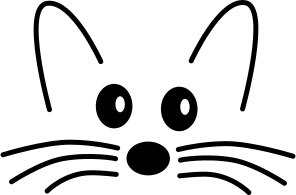
\includegraphics[width=1.4em]{squeak-logo}}}
\iftoshelse{
	\usepackage{marginnote}
		\renewcommand*{\marginfont}{\footnotesize}
	\newcommand{\vartriangleout}{\ifthenelse{\isodd{\thepage}}{\vartriangleright}{\vartriangleleft}}
	\newcommand{\dothisicon}{\fcolorbox{blue!65}{white}{\highlight{$\vartriangleout$}}}
	\newcommand{\dothis}[1]{%
		\noindent\par\noindent
		{\reversemarginpar
			\marginnote{\fcolorbox{blue!65}{white}{\highlight{$\vartriangleout$}}}}
		%\MarginLabel{do this}
		\noindent\emph{#1}
		\nopagebreak}
}{
	\newcommand{\dothisicon}{\raisebox{-.5ex}{
\includegraphics[height=1.2em]{pharo}}}
	\newcommand{\dothis}[1]{%
		\medskip
		\noindent\dothisicon
		\ifx#1\empty\else\quad\emph{#1}\fi
		\par\smallskip\nopagebreak}
}
%===> NEW VERSION <===
% NB: To use this in an individual chapter, you must set:
%\graphicspath{{figures/} {../figures/}}
% at the head of the chapter.  Don't forget the final /
%=============================================================
%:Reader hints (hint)
%
% Indicates a non-obvious consequence 
\newcommand{\hint}[1]{\vspace{1ex}\noindent\fbox{\textsc{Hint}} \emph{#1}}
%=================================================================
% graphics for Morphic handles
\newcommand{\grabHandle}{\raisebox{-0.2ex}{
\includegraphics[width=1em]{blackHandle}}}
\newcommand{\moveHandle}{\raisebox{-0.2ex}{
\includegraphics[width=1em]{moveHandle}}}
\newcommand{\debugHandle}{\raisebox{-0.2ex}{
\includegraphics[width=1em]{debugHandle}}}
%=============================================================
%:Highlighting Important stuff (doublebox)
%
% From Seaside book ...
\newsavebox{\SavedText}
\newlength{\InnerBoxRule}\setlength{\InnerBoxRule}{.75\fboxrule}
\newlength{\OuterBoxRule}\setlength{\OuterBoxRule}{1.5\fboxrule}
\newlength{\BoxSeparation}\setlength{\BoxSeparation}{1.5\fboxrule}
\addtolength{\BoxSeparation}{.5pt}
\newlength{\SaveBoxSep}\setlength{\SaveBoxSep}{2\fboxsep}
%
\newenvironment{doublebox}{\begin{lrbox}{\SavedText}
    \begin{minipage}{.75\textwidth}}
    {\end{minipage}\end{lrbox}\begin{center}
    \setlength{\fboxsep}{\BoxSeparation}\setlength{\fboxrule}{\OuterBoxRule}
    \fbox{\setlength{\fboxsep}{\SaveBoxSep}\setlength{\fboxrule}{\InnerBoxRule}%
      \fbox{\usebox{\SavedText}}}
  \end{center}}
% Use this:
\newcommand{\important}[1]{\begin{doublebox}#1\end{doublebox}}
%=============================================================
%:Section depth
\setcounter{secnumdepth}{2}
%% for this to happen start the file with
%\ifx\wholebook\relax\else
%% $Author$
% $Date$
% $Revision$

% HISTORY:
% 2006-10-31 - Oscar code macros
% ...

%=============================================================
% NB: documentclass must be set in main document.
% Allows book to be generated in multiple formats.
%=============================================================
%:Packages
\usepackage[T1]{fontenc}  %%%%%% really important to get the code directly in the text!
\usepackage{lmodern}
%\usepackage[scaled=0.85]{bookmanx} % needs another scale factor if used with \renewcommand{\sfdefault}{cmbr}
\usepackage{palatino}
\usepackage[scaled=0.85]{helvet}
\usepackage{microtype}
\usepackage{graphicx}
\usepackage{theorem}
\usepackage[english]{babel}
% ON: pdfsync breaks the use of p{width} for tabular columns!
\ifdefined\usepdfsync\usepackage{pdfsync}\fi % Requires texlive 2007
%=============================================================
%:More packages
%Stef should check which ones are used!
%\usepackage{picinpar}
%\usepackage{layout}
%\usepackage{color}
%\usepackage{enum}
%\usepackage{a4wide}
% \usepackage{fancyhdr}
\usepackage{ifthen}
\usepackage{float}
\usepackage{longtable}
\usepackage{makeidx}
\usepackage[nottoc]{tocbibind}
\usepackage{multicol}
\usepackage{booktabs}	% book-style tables
\usepackage{topcapt}	% enables \topcaption
\usepackage{multirow}
\usepackage{tabularx}
%\usepackage[bottom]{footmisc}
\usepackage{xspace}
\usepackage{alltt}
\usepackage{amssymb,textcomp}
\usepackage[usenames,dvipsnames]{color}
%\usepackage{colortbl}
\usepackage[hang]{subfigure}\makeatletter\def\p@subfigure{\thefigure\,}\makeatother
\usepackage{rotating}
\usepackage{enumitem}	% apb: allows more control over tags in enumerations
\usepackage{verbatim}     % for comment environment
\usepackage{varioref}	% for page references that work
\labelformat{footnote}{\thechapter--#1} % to distinguish citations from jurabib
\usepackage{needspace}
\usepackage{isodateo} % enable \isodate
\usepackage[newparttoc]{titlesec}
\usepackage{titletoc}
\usepackage{wrapfig}
\usepackage[
	super,
	citefull=first,
	authorformat={allreversed,and},
	titleformat={commasep,italic}
]{jurabib} % citations as footnotes
\usepackage[
	colorlinks=true,
	linkcolor=black,
	urlcolor=black,
	citecolor=black
]{hyperref}   % should come last
%=============================================================
%:PDF version
\pdfminorversion=3 % Set PDF to 1.3 for Lulu
%=============================================================
%:URL style
\makeatletter
\def\url@leostyle{%
  \@ifundefined{selectfont}{\def\UrlFont{\sf}}{\def\UrlFont{\sffamily}}}
\makeatother
% Now actually use the newly defined style.
\urlstyle{leo}
%=============================================================
%:Booleans
\newboolean{lulu}
\setboolean{lulu}{false}
\newcommand{\ifluluelse}[2]{\ifthenelse{\boolean{lulu}}{#1}{#2}}
%=============================================================
%:Names
\newcommand{\SUnit}{SUnit\xspace}
\newcommand{\sunit}{SUnit\xspace}
\newcommand{\xUnit}{$x$Unit\xspace}
\newcommand{\JUnit}{JUnit\xspace}
\newcommand{\st}{Smalltalk\xspace}
\newcommand{\pharo}{Pharo\xspace} % Use this, not \Pharo
%\newcommand{\sqmap}{SqueakMap\xspace}
\newcommand{\squeak}{Squeak\xspace} % use this, not \Squeak or \sq
\newcommand{\sqsrc}{SqueakSource\xspace}
\newcommand{\sbe}{\url{http://SqueakByExample.org}\xspace}
\newcommand{\pharoweb}{\url{http://pharo-project.org}\xspace}
\newcommand{\pbe}{\url{http://PharoByExample.org}\xspace}
\newcommand{\sba}{\url{http://SquareBracketAssociates.org}\xspace}
\newcommand{\bam}{\lct{Bounc\-ing\-Atoms\-Morph}\xspace}
%=============================================================
%:Markup macros for proof-reading
\usepackage[normalem]{ulem} % for \sout
\usepackage{xcolor}
\newcommand{\ra}{$\rightarrow$}
\newcommand{\ugh}[1]{\textcolor{red}{\uwave{#1}}} % please rephrase
\newcommand{\ins}[1]{\textcolor{blue}{\uline{#1}}} % please insert
\newcommand{\del}[1]{\textcolor{red}{\sout{#1}}} % please delete
\newcommand{\chg}[2]{\textcolor{red}{\sout{#1}}{\ra}\textcolor{blue}{\uline{#2}}} % please change
%=============================================================
%:Editorial comment macros
%\newcommand{\nnbb}[2]{
%    % \fbox{\bfseries\sffamily\scriptsize#1}
%    \fcolorbox{gray}{yellow}{\bfseries\sffamily\scriptsize#1}
%    {\sf\small$\blacktriangleright$\textit{#2}$\blacktriangleleft$}
%   }
\newcommand{\yellowbox}[1]{\fcolorbox{gray}{yellow}{\bfseries\sffamily\scriptsize#1}}
\newcommand{\triangles}[1]{{\sf\small$\blacktriangleright$\textit{#1}$\blacktriangleleft$}}
\newcommand{\nnbb}[2]{\yellowbox{#1} \triangles{#2}}
\newcommand{\fix}{\yellowbox{FIX!}}
\newcommand{\here}{\yellowbox{CONTINUE HERE!}}
% editor macros
\newcommand{\ab}[1]{\nnbb{Andrew}{#1}} % Black
\newcommand{\sd}[1]{\nnbb{St\'{e}f}{#1}} % Ducasse
\newcommand{\md}[1]{\nnbb{Marcus}{#1}} % Denker
\newcommand{\on}[1]{\nnbb{Oscar}{#1}} % Nierstrasz
\newcommand{\damien}[1]{\nnbb{Damien}{#1}} % Pollet
\newcommand{\lr}[1]{\nnbb{Lukas}{#1}} % Renggli
\newcommand{\orla}[1]{\nnbb{Orla}{#1}} % Greevy
\newcommand{\alex}[1]{\nnbb{Alex}{#1}} % Bergel
\newcommand{\alx}[1]{\nnbb{Alex}{#1}} % Bergel
\newcommand{\dr}[1]{\nnbb{David}{#1}} % Roethlisberger
\newcommand{\ja}[1]{\nnbb{Jannik}{#1}} % Laval
\newcommand{\jr}[1]{\nnbb{Jorge}{#1}} % Ressia
\newcommand{\fp}[1]{\nnbb{Fabrizio}{#1}} % Perin
\newcommand{\michael}[1]{\nnbb{Michael}{#1}} % Davies
\newcommand{\ew}[1]{\nnbb{Erwann}{#1}} % Wernli
\newcommand{\mb}[1]{\nnbb{Martial}{#1}} % Boniou
\newcommand{\hw}[1]{\nnbb{Hernan}{#1}} % Wilkinson
%=============================================================
%:Abbreviation macros
\newcommand{\ie}{\emph{i.e.},\xspace}
\newcommand{\eg}{\emph{e.g.},\xspace}
\newcommand{\etc}{etc.\xspace}
%=============================================================
%:Cross reference macros
\newcommand{\charef}[1]{Chapter~\ref{cha:#1}\xspace}
\newcommand{\secref}[1]{Section~\ref{sec:#1}\xspace}
\newcommand{\figref}[1]{Figure~\ref{fig:#1}\xspace}
\newcommand{\Figref}[1]{Figure~\ref{fig:#1}\xspace}
\newcommand{\appref}[1]{Appendix~\ref{app:#1}\xspace}
\newcommand{\tabref}[1]{Table~\ref{tab:#1}\xspace}
\newcommand{\faqref}[1]{FAQ~\ref{faq:#1}, p.~\pageref{faq:#1}\xspace}
% APB: I removed trailing \xspace commands from these macros because
% \xspace mostly doesn't work.  If you want a space after your
% references, type one!
% ON: xspace has always worked just fine for me!  Please leave them in.
%
\newcommand{\ruleref}[1]{\ref{rule:#1}\xspace}
%
\newcommand{\egref}[1]{example~\ref{eg:#1}\xspace}
\newcommand{\Egref}[1]{Example~\ref{eg:#1}\xspace}
%
\newcommand{\scrref}[1]{script~\ref{scr:#1}\xspace}
\newcommand{\Scrref}[1]{Script~\ref{scr:#1}\xspace}
\newcommand{\tscrref}[1]{the script~\ref{scr:#1}\xspace}
\newcommand{\Tscrref}[1]{The script~\ref{scr:#1}\xspace}
%
\newcommand{\mthref}[1]{method~\ref{mth:#1}\xspace}
\newcommand{\mthsref}[1]{methods~\ref{mth:#1}\xspace}
\newcommand{\Mthref}[1]{Method~\ref{mth:#1}\xspace}
\newcommand{\tmthref}[1]{the method~\ref{mth:#1}\xspace}
\newcommand{\Tmthref}[1]{The method~\ref{mth:#1}\xspace}
%
\newcommand{\clsref}[1]{class~\ref{cls:#1}\xspace}
\newcommand{\tclsref}[1]{the class~\ref{cls:#1}\xspace}
\newcommand{\Tclsref}[1]{The class~\ref{cls:#1}\xspace}

\newcommand{\chalabel}[1]{\label{cha:#1}}
\newcommand{\seclabel}[1]{\label{sec:#1}}
\newcommand{\figlabel}[1]{\label{fig:#1}}
\newcommand{\tablabel}[1]{\label{tab:#1}}
\newcommand{\rulelabel}[1]{\label{rule:#1}}
\newcommand{\eglabel}[1]{\label{eg:#1}}
\newcommand{\scrlabel}[1]{\label{scr:#1}}
\newcommand{\mthlabel}[1]{\label{mth:#1}}
\newcommand{\clslabel}[1]{\label{cls:#1}}
\newcommand{\faqlabel}[1]{\label{faq:#1}}
%=============================================================
%:Menu item macro
% for menu items, so we can change our minds on how to print them! (apb)
\definecolor{lightgray}{gray}{0.89}
\newcommand{\menu}[1]{{%
	\setlength{\fboxsep}{0pt}%
	\colorbox{lightgray}{{{\upshape\sffamily\strut \,#1\,}}}}}
\newcommand{\link}[1]{{%
	\fontfamily{lmr}\selectfont
 	\upshape{\sffamily \underline{#1}}}}
% For submenu items:
\newcommand{\go}{\,$\triangleright$\,}
% \newcommand{\go}{\,$\blacktriangleright$\,}
% For keyboard shortcuts:
%\newcommand{\short}[1]{\mbox{$\langle${\sc CMD}$\rangle$-#1}\xspace}
\newcommand{\short}[1]{\mbox{{\sc cmd}\hspace{0.08em}--\hspace{0.09em}#1}\xspace}
% For buttons:
\newcommand{\button}[1]{{%
	\setlength{\fboxsep}{0pt}%
	\fbox{{\upshape\sffamily\strut \,#1\,}}}}
% NB: The button macro does not work within captions -- incompatible with xcolor package :-(
\newcommand{\toolsflap}{\textit{Tools} flap\xspace}
%=============================================================
%:Mouse clicks
\newcommand{\click}{click\xspace} % RED
\newcommand{\actclick}{action-click\xspace} % YELLOW
\newcommand{\metaclick}{meta-click\xspace} % BLUE
\newcommand{\Click}{Click\xspace} % RED
\newcommand{\Actclick}{Action-click\xspace} % YELLOW
\newcommand{\Metaclick}{Meta-click\xspace} % BLUE
%=============================================================
%:ToSh macros
\newboolean{tosh}
\setboolean{tosh}{false}
\newcommand{\iftoshelse}[2]{\ifthenelse{\boolean{tosh}}{#1}{#2}}
%=============================================================
%:ToSh colors
%\newcommand{\highlightcolor}{\color{blue!65}}
%\newcommand{\boxcolor}{\color{gray!25}}
\newcommand{\highlight}[1]{\textcolor{blue!65}{#1}}
%\newcommand{\codecolor}{\color{blue!65}}
%%\setlength{\fboxrule}{2pt}
%\newcommand{\asPict}[1]{%
%	{\Large\highlight{#1}}}
%=============================================================
%:Reader cues (do this)
%
% Indicate something the reader should try out.
% \newcommand{\dothisicon}{\raisebox{-.5ex}{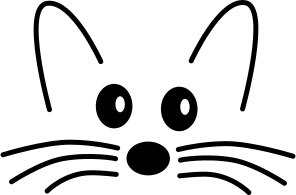
\includegraphics[width=1.4em]{squeak-logo}}}
\iftoshelse{
	\usepackage{marginnote}
		\renewcommand*{\marginfont}{\footnotesize}
	\newcommand{\vartriangleout}{\ifthenelse{\isodd{\thepage}}{\vartriangleright}{\vartriangleleft}}
	\newcommand{\dothisicon}{\fcolorbox{blue!65}{white}{\highlight{$\vartriangleout$}}}
	\newcommand{\dothis}[1]{%
		\noindent\par\noindent
		{\reversemarginpar
			\marginnote{\fcolorbox{blue!65}{white}{\highlight{$\vartriangleout$}}}}
		%\MarginLabel{do this}
		\noindent\emph{#1}
		\nopagebreak}
}{
	\newcommand{\dothisicon}{\raisebox{-.5ex}{
\includegraphics[height=1.2em]{pharo}}}
	\newcommand{\dothis}[1]{%
		\medskip
		\noindent\dothisicon
		\ifx#1\empty\else\quad\emph{#1}\fi
		\par\smallskip\nopagebreak}
}
%===> NEW VERSION <===
% NB: To use this in an individual chapter, you must set:
%\graphicspath{{figures/} {../figures/}}
% at the head of the chapter.  Don't forget the final /
%=============================================================
%:Reader hints (hint)
%
% Indicates a non-obvious consequence 
\newcommand{\hint}[1]{\vspace{1ex}\noindent\fbox{\textsc{Hint}} \emph{#1}}
%=================================================================
% graphics for Morphic handles
\newcommand{\grabHandle}{\raisebox{-0.2ex}{
\includegraphics[width=1em]{blackHandle}}}
\newcommand{\moveHandle}{\raisebox{-0.2ex}{
\includegraphics[width=1em]{moveHandle}}}
\newcommand{\debugHandle}{\raisebox{-0.2ex}{
\includegraphics[width=1em]{debugHandle}}}
%=============================================================
%:Highlighting Important stuff (doublebox)
%
% From Seaside book ...
\newsavebox{\SavedText}
\newlength{\InnerBoxRule}\setlength{\InnerBoxRule}{.75\fboxrule}
\newlength{\OuterBoxRule}\setlength{\OuterBoxRule}{1.5\fboxrule}
\newlength{\BoxSeparation}\setlength{\BoxSeparation}{1.5\fboxrule}
\addtolength{\BoxSeparation}{.5pt}
\newlength{\SaveBoxSep}\setlength{\SaveBoxSep}{2\fboxsep}
%
\newenvironment{doublebox}{\begin{lrbox}{\SavedText}
    \begin{minipage}{.75\textwidth}}
    {\end{minipage}\end{lrbox}\begin{center}
    \setlength{\fboxsep}{\BoxSeparation}\setlength{\fboxrule}{\OuterBoxRule}
    \fbox{\setlength{\fboxsep}{\SaveBoxSep}\setlength{\fboxrule}{\InnerBoxRule}%
      \fbox{\usebox{\SavedText}}}
  \end{center}}
% Use this:
\newcommand{\important}[1]{\begin{doublebox}#1\end{doublebox}}
%=============================================================
%:Section depth
\setcounter{secnumdepth}{2}
%% for this to happen start the file with
%\ifx\wholebook\relax\else
%% $Author$
% $Date$
% $Revision$

% HISTORY:
% 2006-10-31 - Oscar code macros
% ...

%=============================================================
% NB: documentclass must be set in main document.
% Allows book to be generated in multiple formats.
%=============================================================
%:Packages
\usepackage[T1]{fontenc}  %%%%%% really important to get the code directly in the text!
\usepackage{lmodern}
%\usepackage[scaled=0.85]{bookmanx} % needs another scale factor if used with \renewcommand{\sfdefault}{cmbr}
\usepackage{palatino}
\usepackage[scaled=0.85]{helvet}
\usepackage{microtype}
\usepackage{graphicx}
\usepackage{theorem}
\usepackage[english]{babel}
% ON: pdfsync breaks the use of p{width} for tabular columns!
\ifdefined\usepdfsync\usepackage{pdfsync}\fi % Requires texlive 2007
%=============================================================
%:More packages
%Stef should check which ones are used!
%\usepackage{picinpar}
%\usepackage{layout}
%\usepackage{color}
%\usepackage{enum}
%\usepackage{a4wide}
% \usepackage{fancyhdr}
\usepackage{ifthen}
\usepackage{float}
\usepackage{longtable}
\usepackage{makeidx}
\usepackage[nottoc]{tocbibind}
\usepackage{multicol}
\usepackage{booktabs}	% book-style tables
\usepackage{topcapt}	% enables \topcaption
\usepackage{multirow}
\usepackage{tabularx}
%\usepackage[bottom]{footmisc}
\usepackage{xspace}
\usepackage{alltt}
\usepackage{amssymb,textcomp}
\usepackage[usenames,dvipsnames]{color}
%\usepackage{colortbl}
\usepackage[hang]{subfigure}\makeatletter\def\p@subfigure{\thefigure\,}\makeatother
\usepackage{rotating}
\usepackage{enumitem}	% apb: allows more control over tags in enumerations
\usepackage{verbatim}     % for comment environment
\usepackage{varioref}	% for page references that work
\labelformat{footnote}{\thechapter--#1} % to distinguish citations from jurabib
\usepackage{needspace}
\usepackage{isodateo} % enable \isodate
\usepackage[newparttoc]{titlesec}
\usepackage{titletoc}
\usepackage{wrapfig}
\usepackage[
	super,
	citefull=first,
	authorformat={allreversed,and},
	titleformat={commasep,italic}
]{jurabib} % citations as footnotes
\usepackage[
	colorlinks=true,
	linkcolor=black,
	urlcolor=black,
	citecolor=black
]{hyperref}   % should come last
%=============================================================
%:PDF version
\pdfminorversion=3 % Set PDF to 1.3 for Lulu
%=============================================================
%:URL style
\makeatletter
\def\url@leostyle{%
  \@ifundefined{selectfont}{\def\UrlFont{\sf}}{\def\UrlFont{\sffamily}}}
\makeatother
% Now actually use the newly defined style.
\urlstyle{leo}
%=============================================================
%:Booleans
\newboolean{lulu}
\setboolean{lulu}{false}
\newcommand{\ifluluelse}[2]{\ifthenelse{\boolean{lulu}}{#1}{#2}}
%=============================================================
%:Names
\newcommand{\SUnit}{SUnit\xspace}
\newcommand{\sunit}{SUnit\xspace}
\newcommand{\xUnit}{$x$Unit\xspace}
\newcommand{\JUnit}{JUnit\xspace}
\newcommand{\st}{Smalltalk\xspace}
\newcommand{\pharo}{Pharo\xspace} % Use this, not \Pharo
%\newcommand{\sqmap}{SqueakMap\xspace}
\newcommand{\squeak}{Squeak\xspace} % use this, not \Squeak or \sq
\newcommand{\sqsrc}{SqueakSource\xspace}
\newcommand{\sbe}{\url{http://SqueakByExample.org}\xspace}
\newcommand{\pharoweb}{\url{http://pharo-project.org}\xspace}
\newcommand{\pbe}{\url{http://PharoByExample.org}\xspace}
\newcommand{\sba}{\url{http://SquareBracketAssociates.org}\xspace}
\newcommand{\bam}{\lct{Bounc\-ing\-Atoms\-Morph}\xspace}
%=============================================================
%:Markup macros for proof-reading
\usepackage[normalem]{ulem} % for \sout
\usepackage{xcolor}
\newcommand{\ra}{$\rightarrow$}
\newcommand{\ugh}[1]{\textcolor{red}{\uwave{#1}}} % please rephrase
\newcommand{\ins}[1]{\textcolor{blue}{\uline{#1}}} % please insert
\newcommand{\del}[1]{\textcolor{red}{\sout{#1}}} % please delete
\newcommand{\chg}[2]{\textcolor{red}{\sout{#1}}{\ra}\textcolor{blue}{\uline{#2}}} % please change
%=============================================================
%:Editorial comment macros
%\newcommand{\nnbb}[2]{
%    % \fbox{\bfseries\sffamily\scriptsize#1}
%    \fcolorbox{gray}{yellow}{\bfseries\sffamily\scriptsize#1}
%    {\sf\small$\blacktriangleright$\textit{#2}$\blacktriangleleft$}
%   }
\newcommand{\yellowbox}[1]{\fcolorbox{gray}{yellow}{\bfseries\sffamily\scriptsize#1}}
\newcommand{\triangles}[1]{{\sf\small$\blacktriangleright$\textit{#1}$\blacktriangleleft$}}
\newcommand{\nnbb}[2]{\yellowbox{#1} \triangles{#2}}
\newcommand{\fix}{\yellowbox{FIX!}}
\newcommand{\here}{\yellowbox{CONTINUE HERE!}}
% editor macros
\newcommand{\ab}[1]{\nnbb{Andrew}{#1}} % Black
\newcommand{\sd}[1]{\nnbb{St\'{e}f}{#1}} % Ducasse
\newcommand{\md}[1]{\nnbb{Marcus}{#1}} % Denker
\newcommand{\on}[1]{\nnbb{Oscar}{#1}} % Nierstrasz
\newcommand{\damien}[1]{\nnbb{Damien}{#1}} % Pollet
\newcommand{\lr}[1]{\nnbb{Lukas}{#1}} % Renggli
\newcommand{\orla}[1]{\nnbb{Orla}{#1}} % Greevy
\newcommand{\alex}[1]{\nnbb{Alex}{#1}} % Bergel
\newcommand{\alx}[1]{\nnbb{Alex}{#1}} % Bergel
\newcommand{\dr}[1]{\nnbb{David}{#1}} % Roethlisberger
\newcommand{\ja}[1]{\nnbb{Jannik}{#1}} % Laval
\newcommand{\jr}[1]{\nnbb{Jorge}{#1}} % Ressia
\newcommand{\fp}[1]{\nnbb{Fabrizio}{#1}} % Perin
\newcommand{\michael}[1]{\nnbb{Michael}{#1}} % Davies
\newcommand{\ew}[1]{\nnbb{Erwann}{#1}} % Wernli
\newcommand{\mb}[1]{\nnbb{Martial}{#1}} % Boniou
\newcommand{\hw}[1]{\nnbb{Hernan}{#1}} % Wilkinson
%=============================================================
%:Abbreviation macros
\newcommand{\ie}{\emph{i.e.},\xspace}
\newcommand{\eg}{\emph{e.g.},\xspace}
\newcommand{\etc}{etc.\xspace}
%=============================================================
%:Cross reference macros
\newcommand{\charef}[1]{Chapter~\ref{cha:#1}\xspace}
\newcommand{\secref}[1]{Section~\ref{sec:#1}\xspace}
\newcommand{\figref}[1]{Figure~\ref{fig:#1}\xspace}
\newcommand{\Figref}[1]{Figure~\ref{fig:#1}\xspace}
\newcommand{\appref}[1]{Appendix~\ref{app:#1}\xspace}
\newcommand{\tabref}[1]{Table~\ref{tab:#1}\xspace}
\newcommand{\faqref}[1]{FAQ~\ref{faq:#1}, p.~\pageref{faq:#1}\xspace}
% APB: I removed trailing \xspace commands from these macros because
% \xspace mostly doesn't work.  If you want a space after your
% references, type one!
% ON: xspace has always worked just fine for me!  Please leave them in.
%
\newcommand{\ruleref}[1]{\ref{rule:#1}\xspace}
%
\newcommand{\egref}[1]{example~\ref{eg:#1}\xspace}
\newcommand{\Egref}[1]{Example~\ref{eg:#1}\xspace}
%
\newcommand{\scrref}[1]{script~\ref{scr:#1}\xspace}
\newcommand{\Scrref}[1]{Script~\ref{scr:#1}\xspace}
\newcommand{\tscrref}[1]{the script~\ref{scr:#1}\xspace}
\newcommand{\Tscrref}[1]{The script~\ref{scr:#1}\xspace}
%
\newcommand{\mthref}[1]{method~\ref{mth:#1}\xspace}
\newcommand{\mthsref}[1]{methods~\ref{mth:#1}\xspace}
\newcommand{\Mthref}[1]{Method~\ref{mth:#1}\xspace}
\newcommand{\tmthref}[1]{the method~\ref{mth:#1}\xspace}
\newcommand{\Tmthref}[1]{The method~\ref{mth:#1}\xspace}
%
\newcommand{\clsref}[1]{class~\ref{cls:#1}\xspace}
\newcommand{\tclsref}[1]{the class~\ref{cls:#1}\xspace}
\newcommand{\Tclsref}[1]{The class~\ref{cls:#1}\xspace}

\newcommand{\chalabel}[1]{\label{cha:#1}}
\newcommand{\seclabel}[1]{\label{sec:#1}}
\newcommand{\figlabel}[1]{\label{fig:#1}}
\newcommand{\tablabel}[1]{\label{tab:#1}}
\newcommand{\rulelabel}[1]{\label{rule:#1}}
\newcommand{\eglabel}[1]{\label{eg:#1}}
\newcommand{\scrlabel}[1]{\label{scr:#1}}
\newcommand{\mthlabel}[1]{\label{mth:#1}}
\newcommand{\clslabel}[1]{\label{cls:#1}}
\newcommand{\faqlabel}[1]{\label{faq:#1}}
%=============================================================
%:Menu item macro
% for menu items, so we can change our minds on how to print them! (apb)
\definecolor{lightgray}{gray}{0.89}
\newcommand{\menu}[1]{{%
	\setlength{\fboxsep}{0pt}%
	\colorbox{lightgray}{{{\upshape\sffamily\strut \,#1\,}}}}}
\newcommand{\link}[1]{{%
	\fontfamily{lmr}\selectfont
 	\upshape{\sffamily \underline{#1}}}}
% For submenu items:
\newcommand{\go}{\,$\triangleright$\,}
% \newcommand{\go}{\,$\blacktriangleright$\,}
% For keyboard shortcuts:
%\newcommand{\short}[1]{\mbox{$\langle${\sc CMD}$\rangle$-#1}\xspace}
\newcommand{\short}[1]{\mbox{{\sc cmd}\hspace{0.08em}--\hspace{0.09em}#1}\xspace}
% For buttons:
\newcommand{\button}[1]{{%
	\setlength{\fboxsep}{0pt}%
	\fbox{{\upshape\sffamily\strut \,#1\,}}}}
% NB: The button macro does not work within captions -- incompatible with xcolor package :-(
\newcommand{\toolsflap}{\textit{Tools} flap\xspace}
%=============================================================
%:Mouse clicks
\newcommand{\click}{click\xspace} % RED
\newcommand{\actclick}{action-click\xspace} % YELLOW
\newcommand{\metaclick}{meta-click\xspace} % BLUE
\newcommand{\Click}{Click\xspace} % RED
\newcommand{\Actclick}{Action-click\xspace} % YELLOW
\newcommand{\Metaclick}{Meta-click\xspace} % BLUE
%=============================================================
%:ToSh macros
\newboolean{tosh}
\setboolean{tosh}{false}
\newcommand{\iftoshelse}[2]{\ifthenelse{\boolean{tosh}}{#1}{#2}}
%=============================================================
%:ToSh colors
%\newcommand{\highlightcolor}{\color{blue!65}}
%\newcommand{\boxcolor}{\color{gray!25}}
\newcommand{\highlight}[1]{\textcolor{blue!65}{#1}}
%\newcommand{\codecolor}{\color{blue!65}}
%%\setlength{\fboxrule}{2pt}
%\newcommand{\asPict}[1]{%
%	{\Large\highlight{#1}}}
%=============================================================
%:Reader cues (do this)
%
% Indicate something the reader should try out.
% \newcommand{\dothisicon}{\raisebox{-.5ex}{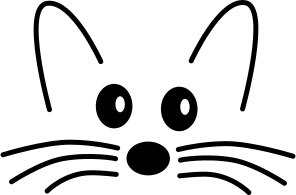
\includegraphics[width=1.4em]{squeak-logo}}}
\iftoshelse{
	\usepackage{marginnote}
		\renewcommand*{\marginfont}{\footnotesize}
	\newcommand{\vartriangleout}{\ifthenelse{\isodd{\thepage}}{\vartriangleright}{\vartriangleleft}}
	\newcommand{\dothisicon}{\fcolorbox{blue!65}{white}{\highlight{$\vartriangleout$}}}
	\newcommand{\dothis}[1]{%
		\noindent\par\noindent
		{\reversemarginpar
			\marginnote{\fcolorbox{blue!65}{white}{\highlight{$\vartriangleout$}}}}
		%\MarginLabel{do this}
		\noindent\emph{#1}
		\nopagebreak}
}{
	\newcommand{\dothisicon}{\raisebox{-.5ex}{
\includegraphics[height=1.2em]{pharo}}}
	\newcommand{\dothis}[1]{%
		\medskip
		\noindent\dothisicon
		\ifx#1\empty\else\quad\emph{#1}\fi
		\par\smallskip\nopagebreak}
}
%===> NEW VERSION <===
% NB: To use this in an individual chapter, you must set:
%\graphicspath{{figures/} {../figures/}}
% at the head of the chapter.  Don't forget the final /
%=============================================================
%:Reader hints (hint)
%
% Indicates a non-obvious consequence 
\newcommand{\hint}[1]{\vspace{1ex}\noindent\fbox{\textsc{Hint}} \emph{#1}}
%=================================================================
% graphics for Morphic handles
\newcommand{\grabHandle}{\raisebox{-0.2ex}{
\includegraphics[width=1em]{blackHandle}}}
\newcommand{\moveHandle}{\raisebox{-0.2ex}{
\includegraphics[width=1em]{moveHandle}}}
\newcommand{\debugHandle}{\raisebox{-0.2ex}{
\includegraphics[width=1em]{debugHandle}}}
%=============================================================
%:Highlighting Important stuff (doublebox)
%
% From Seaside book ...
\newsavebox{\SavedText}
\newlength{\InnerBoxRule}\setlength{\InnerBoxRule}{.75\fboxrule}
\newlength{\OuterBoxRule}\setlength{\OuterBoxRule}{1.5\fboxrule}
\newlength{\BoxSeparation}\setlength{\BoxSeparation}{1.5\fboxrule}
\addtolength{\BoxSeparation}{.5pt}
\newlength{\SaveBoxSep}\setlength{\SaveBoxSep}{2\fboxsep}
%
\newenvironment{doublebox}{\begin{lrbox}{\SavedText}
    \begin{minipage}{.75\textwidth}}
    {\end{minipage}\end{lrbox}\begin{center}
    \setlength{\fboxsep}{\BoxSeparation}\setlength{\fboxrule}{\OuterBoxRule}
    \fbox{\setlength{\fboxsep}{\SaveBoxSep}\setlength{\fboxrule}{\InnerBoxRule}%
      \fbox{\usebox{\SavedText}}}
  \end{center}}
% Use this:
\newcommand{\important}[1]{\begin{doublebox}#1\end{doublebox}}
%=============================================================
%:Section depth
\setcounter{secnumdepth}{2}
%% for this to happen start the file with
%\ifx\wholebook\relax\else
%\input{../common.tex}
%\begin{document}
%\fi
% and terminate by
% \ifx\wholebook\relax\else\end{document}\fi

\DeclareGraphicsExtensions{.pdf, .jpg, .png}
%=============================================================
%:PDF setup
\hypersetup{
%   a4paper,
%   pdfstartview=FitV,
%   colorlinks,
%   linkcolor=darkblue,
%   citecolor=darkblue,
   pdftitle={Pharo by Example},
   pdfauthor={Andrew P. Black, St\'ephane Ducasse,	Oscar Nierstrasz,
Damien Pollet},
   pdfkeywords={Smalltalk, Squeak, Object-Oriented Programming, OOP},
   pdfsubject={Computer Science}
}
%=============================================================
%:Page layout and appearance
%
% \renewcommand{\headrulewidth}{0pt}
\renewcommand{\chaptermark}[1]{\markboth{#1}{}}
\renewcommand{\sectionmark}[1]{\markright{\thesection\ #1}}
\renewpagestyle{plain}[\small\itshape]{%
	\setheadrule{0pt}%
	\sethead[][][]{}{}{}%
	\setfoot[][][]{}{}{}}
\renewpagestyle{headings}[\small\itshape]{%
	\setheadrule{0pt}%
	\setmarks{chapter}{section}%
	\sethead[\thepage][][\chaptertitle]{\sectiontitle}{}{\thepage}%
	\setfoot[][][]{}{}{}}
%=============================================================
%:Title section setup and TOC numbering depth
\setcounter{secnumdepth}{1}
\setcounter{tocdepth}{1}
\titleformat{\part}[display]{\centering}{\huge\partname\ \thepart}{1em}{\Huge\textbf}[]
\titleformat{\chapter}[display]{}{\huge\chaptertitlename\ \thechapter}{1em}{\Huge\raggedright\textbf}[]
\titlecontents{part}[3pc]{%
		\pagebreak[2]\addvspace{1em plus.4em minus.2em}%
		\leavevmode\large\bfseries}
	{\contentslabel{3pc}}{\hspace*{-3pc}}
	{}[\nopagebreak]
\titlecontents{chapter}[3pc]{%
		\pagebreak[0]\addvspace{1em plus.2em minus.2em}%
		\leavevmode\bfseries}
	{\contentslabel{3pc}}{}
	{\hfill\contentspage}[\nopagebreak]
\dottedcontents{section}[3pc]{}{3pc}{1pc}
\dottedcontents{subsection}[3pc]{}{0pc}{1pc}
% \dottedcontents{subsection}[4.5em]{}{0pt}{1pc}
% Make \cleardoublepage insert really blank pages http://www.tex.ac.uk/cgi-bin/texfaq2html?label=reallyblank
\let\origdoublepage\cleardoublepage
\newcommand{\clearemptydoublepage}{%
  \clearpage
  {\pagestyle{empty}\origdoublepage}}
\let\cleardoublepage\clearemptydoublepage % see http://www.tex.ac.uk/cgi-bin/texfaq2html?label=patch
%=============================================================
%:FAQ macros (for FAQ chapter)
\newtheorem{faq}{FAQ}
\newcommand{\answer}{\paragraph{Answer}\ }
%=============================================================
%:Listings package configuration
% \newcommand{\caret}{\makebox{\raisebox{0.4ex}{\footnotesize{$\wedge$}}}}
\newcommand{\caret}{\^\,}
\newcommand{\escape}{{\sf \textbackslash}}
\definecolor{source}{gray}{0.95}
\usepackage{listings}
\lstdefinelanguage{Smalltalk}{
%  morekeywords={self,super,true,false,nil,thisContext}, % This is overkill
  morestring=[d]',
  morecomment=[s]{"}{"},
  alsoletter={\#:},
  escapechar={!},
  literate=
    {BANG}{!}1
    {CARET}{\^}1
    {UNDERSCORE}{\_}1
    {\\st}{Smalltalk}9 % convenience -- in case \st occurs in code
    % {'}{{\textquotesingle}}1 % replaced by upquote=true in \lstset
    {_}{{$\leftarrow$}}1
    {>>>}{{\sep}}1
    {^}{{$\uparrow$}}1
    {~}{{$\sim$}}1
    {-}{{\textminus}}1 %{-}{\hspace{-0.13em}}{-}}1  % the goal is to make - the same width as +
    % {+}{\sf+}1 %{\raisebox{0.08ex}{+}}}1      % and to raise + off the baseline to match -
    {-->}{{\quad$\longrightarrow$\quad}}3
	, % Don't forget the comma at the end!
  tabsize=4
}[keywords,comments,strings]

\lstset{language=Smalltalk,
	basicstyle=\sffamily,
	keywordstyle=\color{black}\bfseries,
	% stringstyle=\ttfamily, % Ugly! do we really want this? -- on
	mathescape=true,
	showstringspaces=false,
	keepspaces=true,
	breaklines=true,
	breakautoindent=true,
	backgroundcolor=\color{source},
	lineskip={-1pt}, % Ugly hack
	upquote=true, % straight quote; requires textcomp package
	columns=fullflexible} % no fixed width fonts
% In-line code (literal)
% Normally use this for all in-line code:
\newcommand{\ct}{\lstinline[mathescape=false,backgroundcolor=\color{white},basicstyle={\sffamily\upshape}]}
% apb 2007.8.28 added the \upshape declaration to avoid getting italicized code in \dothis{ } sections.
% In-line code (latex enabled)
% Use this only in special situations where \ct does not work
% (within section headings ...):
\newcommand{\lct}[1]{{\textsf{\textup{#1}}}}
% Use these for system categories and protocols:
\newcommand{\scat}[1]{\emph{\textsf{#1}}\xspace}
\newcommand{\pkg}[1]{\emph{\textsf{#1}}\xspace}
\newcommand{\prot}[1]{\emph{\textsf{#1}}\xspace}
% Code environments
% NB: the arg is for tests
% Only code and example environments may be tests
\lstnewenvironment{code}[1]{%
	\lstset{%
		% frame=lines,
		frame=single,
		framerule=0pt,
		mathescape=false
	}
}{}
\def\ignoredollar#1{}
%=============================================================
%:Code environments (method, script ...)
% NB: the third arg is for tests
% Only code and example environments may be tests
\lstnewenvironment{example}[3][defaultlabel]{%
	\renewcommand{\lstlistingname}{Example}%
	\lstset{
		% frame=lines,
		frame=single,
		framerule=0pt,
		mathescape=false,
		caption={\emph{#2}},
		label={eg:#1}
	}
}{}
\lstnewenvironment{script}[2][defaultlabel]{%
\renewcommand{\lstlistingname}{Script}%
	\lstset{
		% frame=lines,
		frame=single,
		framerule=0pt,
		mathescape=false,
		name={Script},
		caption={\emph{#2}},
		label={scr:#1}
	}
}{}
\lstnewenvironment{method}[2][defaultlabel]{%
	\renewcommand{\lstlistingname}{Method}%
	\lstset{
		% frame=lines,
		frame=single,
		framerule=0pt,
		mathescape=false,
		name={Method},
		caption={\emph{#2}},
		label={mth:#1}
	}
}{}
\lstnewenvironment{methods}[2][defaultlabel]{% just for multiple methods at once
	\renewcommand{\lstlistingname}{Methods}%
	\lstset{
		% frame=lines,
		frame=single,
		framerule=0pt,
		mathescape=false,
		name={Method},
		caption={\emph{#2}},
		label={mth:#1}
	}
}{}
\lstnewenvironment{numMethod}[2][defaultlabel]{%
	\renewcommand{\lstlistingname}{Method}%
	\lstset{
		numbers=left,
		numberstyle={\tiny\sffamily},
		% frame=lines,
		frame=single,
		framerule=0pt,
		mathescape=false,
		name={Method},
		caption={\emph{#2}},
		label={mth:#1}
	}
}{}
\lstnewenvironment{classdef}[2][defaultlabel]{%
	\renewcommand{\lstlistingname}{Class}%
	\lstset{
		% frame=lines,
		frame=single,
		framerule=0pt,
		mathescape=false,
		name={Class},
		caption={\emph{#2}},
		label={cls:#1}
	}
}{}
%=============================================================
%:Reserving space
% Usually need one more line than the actual lines of code
\newcommand{\needlines}[1]{\Needspace{#1\baselineskip}}
%=============================================================
%:Indexing macros
% Macros ending with "ind" generate text as well as an index entry
% Macros ending with "index" *only* generate an index entry
\newcommand{\ind}[1]{\index{#1}#1\xspace} % plain text
\newcommand{\subind}[2]{\index{#1!#2}#2\xspace} % show #2, subindex under #1
\newcommand{\emphind}[1]{\index{#1}\emph{#1}\xspace} % emph #1
\newcommand{\emphsubind}[2]{\index{#1!#2}\emph{#2}\xspace} % show emph #2, subindex inder #1
\newcommand{\scatind}[1]{\index{#1@\textsf{#1} (category)}\scat{#1}} % category
\newcommand{\pkgind}[1]{\index{#1@\textsf{#1} (package)}\pkg{#1}} % package
\newcommand{\protind}[1]{\index{#1@\textsf{#1} (protocol)}\prot{#1}} % protocol
\newcommand{\clsind}[1]{\index{#1@\textsf{#1} (class)}\ct{#1}\xspace}
% \newcommand{\clsind}[1]{\index{#1!\#@(class)}\ct{#1}\xspace} % class
\newcommand{\clsindplural}[1]{\index{#1!\#@(class)}\ct{#1}s\xspace} % class
\newcommand{\cvind}[1]{\index{#1@\textsf{#1} (class variable)}\ct{#1}\xspace} % class var
\newcommand{\glbind}[1]{\index{#1@\textsf{#1} (global)}\ct{#1}\xspace} % global
\newcommand{\patind}[1]{\index{#1@#1 (pattern)}\ct{#1}\xspace} % pattern
\newcommand{\pvind}[1]{\index{#1@\textsf{#1} (pseudo variable)}\ct{#1}\xspace} % pseudo var
\newcommand{\clsmthind}[2]{\index{#1!#2@\ct{#2}}\ct{#1>>>#2}\xspace} % class + method name
\newcommand{\mthind}[2]{\index{#1!#2@\ct{#2}}\ct{#2}\xspace} % show method name only
\newcommand{\lmthind}[2]{\index{#1!#2@\ct{#2}}\lct{#2}\xspace} % show method name only
\newcommand{\cmind}[2]{\index{#1!#2@\ct{#2}}\ct{#1>>>#2}\xspace} % show class>>method
\newcommand{\lcmind}[2]{\index{#1!#2@\ct{#2}}\lct{#1>>>#2}\xspace} % show class>>method
\newcommand{\toolsflapind}{\index{Tools flap}\toolsflap} % index tools flap
% The following only generate an index entry:
% \newcommand{\clsindex}[1]{\index{#1@\textsf{#1} (class)}}
\newcommand{\clsindex}[1]{\index{#1!\#@(class)}} % class
\newcommand{\mthindex}[2]{\index{#1!#2@\ct{#2}}} % method
\newcommand{\cmindex}[2]{\index{#1!#2@\ct{#2}}} % class>>method
\newcommand{\cvindex}[1]{\index{#1@\textsf{#1} (class variable)}} % class var
\newcommand{\glbindex}[1]{\index{#1@\textsf{#1} (global)}}% global
\newcommand{\pvindex}[1]{\index{#1@\textsf{#1} (pseudo variable)}}% pseudo var
\newcommand{\seeindex}[2]{\index{#1|see{#2}}} % #1, see #2
\newcommand{\scatindex}[1]{\index{#1@\textsf{#1} (category)}} % category
\newcommand{\pkgindex}[1]{\index{#1@\textsf{#1} (package)}} % package
\newcommand{\protindex}[1]{\index{#1@\textsf{#1} (protocol)}} % protocol
% How can we have the main entry page numbers in bold yet not break the hyperlink?
\newcommand{\boldidx}[1]{{\bf #1}} % breaks hyperlink
%\newcommand{\indmain}[1]{\index{#1|boldidx}#1\xspace} % plain text, main entry
%\newcommand{\emphsubindmain}[2]{\index{#1!#2|boldidx}\emph{#2}\xspace} % subindex, main entry
%\newcommand{\subindmain}[2]{\index{#1!#2|boldidx}#2\xspace} % subindex, main entry
%\newcommand{\clsindmain}[1]{\index{#1@\textsf{#1} (class)|boldidx}\ct{#1}\xspace}
%\newcommand{\clsindmain}[1]{\index{#1!\#@(class)|boldidx}\ct{#1}\xspace} % class main
%\newcommand{\indexmain}[1]{\index{#1|boldidx}} % main index entry only
\newcommand{\indmain}[1]{\index{#1}#1\xspace} % The main index entry for this item
\newcommand{\emphsubindmain}[2]{\index{#1!#2}\emph{#2}\xspace} % subindex, main entry
\newcommand{\subindmain}[2]{\index{#1!#2}#2\xspace} % subindex, main entry
%\newcommand{\clsindmain}[1]{\index{#1@\textsf{#1} (class)}\ct{#1}\xspace}
\newcommand{\clsindmain}[1]{\index{#1!\#@(class)}\ct{#1}\xspace} % class main
\newcommand{\clsindexmain}[1]{\index{#1!\#@(class)}} % class main index only
\newcommand{\indexmain}[1]{\index{#1}} 
%=============================================================
%:Code macros
% some constants
\newcommand{\codesize}{\small}
\newcommand{\codefont}{\sffamily}
%\newcommand{\cat}[1]{\textit{In category #1}}%%To remove later
\newlength{\scriptindent}
\setlength{\scriptindent}{.3cm}
%% Method presentation constants
\newlength{\methodindent}
\newlength{\methodwordlength}
\newlength{\aftermethod}
\setlength{\methodindent}{0.2cm}
\settowidth{\methodwordlength}{\ M\'ethode\ }
%=============================================================
%:Smalltalk macros
%\newcommand{\sep}{{$\gg$}}
\newcommand{\sep}{\mbox{>>}}
\newcommand{\self}{\lct{self}\xspace}
\newcommand{\super}{\lct{super}\xspace}
\newcommand{\nil}{\lct{nil}\xspace}
%=============================================================
% be less conservative about float placement
% these commands are from http://www.tex.ac.uk/cgi-bin/texfaq2html?label=floats
\renewcommand{\topfraction}{.9}
\renewcommand{\bottomfraction}{.9}
\renewcommand{\textfraction}{.1}
\renewcommand{\floatpagefraction}{.85}
\renewcommand{\dbltopfraction}{.66}
\renewcommand{\dblfloatpagefraction}{.85}
\setcounter{topnumber}{9}
\setcounter{bottomnumber}{9}
\setcounter{totalnumber}{20}
\setcounter{dbltopnumber}{9}
%=============================================================
% apb doesn't like paragraphs to run in to each other without a break
\parskip 1ex
%=============================================================
%:Stuff to check, merge or deprecate
%\setlength{\marginparsep}{2mm}
%\renewcommand{\baselinestretch}{1.1}
%=============================================================

%\begin{document}
%\fi
% and terminate by
% \ifx\wholebook\relax\else\end{document}\fi

\DeclareGraphicsExtensions{.pdf, .jpg, .png}
%=============================================================
%:PDF setup
\hypersetup{
%   a4paper,
%   pdfstartview=FitV,
%   colorlinks,
%   linkcolor=darkblue,
%   citecolor=darkblue,
   pdftitle={Pharo by Example},
   pdfauthor={Andrew P. Black, St\'ephane Ducasse,	Oscar Nierstrasz,
Damien Pollet},
   pdfkeywords={Smalltalk, Squeak, Object-Oriented Programming, OOP},
   pdfsubject={Computer Science}
}
%=============================================================
%:Page layout and appearance
%
% \renewcommand{\headrulewidth}{0pt}
\renewcommand{\chaptermark}[1]{\markboth{#1}{}}
\renewcommand{\sectionmark}[1]{\markright{\thesection\ #1}}
\renewpagestyle{plain}[\small\itshape]{%
	\setheadrule{0pt}%
	\sethead[][][]{}{}{}%
	\setfoot[][][]{}{}{}}
\renewpagestyle{headings}[\small\itshape]{%
	\setheadrule{0pt}%
	\setmarks{chapter}{section}%
	\sethead[\thepage][][\chaptertitle]{\sectiontitle}{}{\thepage}%
	\setfoot[][][]{}{}{}}
%=============================================================
%:Title section setup and TOC numbering depth
\setcounter{secnumdepth}{1}
\setcounter{tocdepth}{1}
\titleformat{\part}[display]{\centering}{\huge\partname\ \thepart}{1em}{\Huge\textbf}[]
\titleformat{\chapter}[display]{}{\huge\chaptertitlename\ \thechapter}{1em}{\Huge\raggedright\textbf}[]
\titlecontents{part}[3pc]{%
		\pagebreak[2]\addvspace{1em plus.4em minus.2em}%
		\leavevmode\large\bfseries}
	{\contentslabel{3pc}}{\hspace*{-3pc}}
	{}[\nopagebreak]
\titlecontents{chapter}[3pc]{%
		\pagebreak[0]\addvspace{1em plus.2em minus.2em}%
		\leavevmode\bfseries}
	{\contentslabel{3pc}}{}
	{\hfill\contentspage}[\nopagebreak]
\dottedcontents{section}[3pc]{}{3pc}{1pc}
\dottedcontents{subsection}[3pc]{}{0pc}{1pc}
% \dottedcontents{subsection}[4.5em]{}{0pt}{1pc}
% Make \cleardoublepage insert really blank pages http://www.tex.ac.uk/cgi-bin/texfaq2html?label=reallyblank
\let\origdoublepage\cleardoublepage
\newcommand{\clearemptydoublepage}{%
  \clearpage
  {\pagestyle{empty}\origdoublepage}}
\let\cleardoublepage\clearemptydoublepage % see http://www.tex.ac.uk/cgi-bin/texfaq2html?label=patch
%=============================================================
%:FAQ macros (for FAQ chapter)
\newtheorem{faq}{FAQ}
\newcommand{\answer}{\paragraph{Answer}\ }
%=============================================================
%:Listings package configuration
% \newcommand{\caret}{\makebox{\raisebox{0.4ex}{\footnotesize{$\wedge$}}}}
\newcommand{\caret}{\^\,}
\newcommand{\escape}{{\sf \textbackslash}}
\definecolor{source}{gray}{0.95}
\usepackage{listings}
\lstdefinelanguage{Smalltalk}{
%  morekeywords={self,super,true,false,nil,thisContext}, % This is overkill
  morestring=[d]',
  morecomment=[s]{"}{"},
  alsoletter={\#:},
  escapechar={!},
  literate=
    {BANG}{!}1
    {CARET}{\^}1
    {UNDERSCORE}{\_}1
    {\\st}{Smalltalk}9 % convenience -- in case \st occurs in code
    % {'}{{\textquotesingle}}1 % replaced by upquote=true in \lstset
    {_}{{$\leftarrow$}}1
    {>>>}{{\sep}}1
    {^}{{$\uparrow$}}1
    {~}{{$\sim$}}1
    {-}{{\textminus}}1 %{-}{\hspace{-0.13em}}{-}}1  % the goal is to make - the same width as +
    % {+}{\sf+}1 %{\raisebox{0.08ex}{+}}}1      % and to raise + off the baseline to match -
    {-->}{{\quad$\longrightarrow$\quad}}3
	, % Don't forget the comma at the end!
  tabsize=4
}[keywords,comments,strings]

\lstset{language=Smalltalk,
	basicstyle=\sffamily,
	keywordstyle=\color{black}\bfseries,
	% stringstyle=\ttfamily, % Ugly! do we really want this? -- on
	mathescape=true,
	showstringspaces=false,
	keepspaces=true,
	breaklines=true,
	breakautoindent=true,
	backgroundcolor=\color{source},
	lineskip={-1pt}, % Ugly hack
	upquote=true, % straight quote; requires textcomp package
	columns=fullflexible} % no fixed width fonts
% In-line code (literal)
% Normally use this for all in-line code:
\newcommand{\ct}{\lstinline[mathescape=false,backgroundcolor=\color{white},basicstyle={\sffamily\upshape}]}
% apb 2007.8.28 added the \upshape declaration to avoid getting italicized code in \dothis{ } sections.
% In-line code (latex enabled)
% Use this only in special situations where \ct does not work
% (within section headings ...):
\newcommand{\lct}[1]{{\textsf{\textup{#1}}}}
% Use these for system categories and protocols:
\newcommand{\scat}[1]{\emph{\textsf{#1}}\xspace}
\newcommand{\pkg}[1]{\emph{\textsf{#1}}\xspace}
\newcommand{\prot}[1]{\emph{\textsf{#1}}\xspace}
% Code environments
% NB: the arg is for tests
% Only code and example environments may be tests
\lstnewenvironment{code}[1]{%
	\lstset{%
		% frame=lines,
		frame=single,
		framerule=0pt,
		mathescape=false
	}
}{}
\def\ignoredollar#1{}
%=============================================================
%:Code environments (method, script ...)
% NB: the third arg is for tests
% Only code and example environments may be tests
\lstnewenvironment{example}[3][defaultlabel]{%
	\renewcommand{\lstlistingname}{Example}%
	\lstset{
		% frame=lines,
		frame=single,
		framerule=0pt,
		mathescape=false,
		caption={\emph{#2}},
		label={eg:#1}
	}
}{}
\lstnewenvironment{script}[2][defaultlabel]{%
\renewcommand{\lstlistingname}{Script}%
	\lstset{
		% frame=lines,
		frame=single,
		framerule=0pt,
		mathescape=false,
		name={Script},
		caption={\emph{#2}},
		label={scr:#1}
	}
}{}
\lstnewenvironment{method}[2][defaultlabel]{%
	\renewcommand{\lstlistingname}{Method}%
	\lstset{
		% frame=lines,
		frame=single,
		framerule=0pt,
		mathescape=false,
		name={Method},
		caption={\emph{#2}},
		label={mth:#1}
	}
}{}
\lstnewenvironment{methods}[2][defaultlabel]{% just for multiple methods at once
	\renewcommand{\lstlistingname}{Methods}%
	\lstset{
		% frame=lines,
		frame=single,
		framerule=0pt,
		mathescape=false,
		name={Method},
		caption={\emph{#2}},
		label={mth:#1}
	}
}{}
\lstnewenvironment{numMethod}[2][defaultlabel]{%
	\renewcommand{\lstlistingname}{Method}%
	\lstset{
		numbers=left,
		numberstyle={\tiny\sffamily},
		% frame=lines,
		frame=single,
		framerule=0pt,
		mathescape=false,
		name={Method},
		caption={\emph{#2}},
		label={mth:#1}
	}
}{}
\lstnewenvironment{classdef}[2][defaultlabel]{%
	\renewcommand{\lstlistingname}{Class}%
	\lstset{
		% frame=lines,
		frame=single,
		framerule=0pt,
		mathescape=false,
		name={Class},
		caption={\emph{#2}},
		label={cls:#1}
	}
}{}
%=============================================================
%:Reserving space
% Usually need one more line than the actual lines of code
\newcommand{\needlines}[1]{\Needspace{#1\baselineskip}}
%=============================================================
%:Indexing macros
% Macros ending with "ind" generate text as well as an index entry
% Macros ending with "index" *only* generate an index entry
\newcommand{\ind}[1]{\index{#1}#1\xspace} % plain text
\newcommand{\subind}[2]{\index{#1!#2}#2\xspace} % show #2, subindex under #1
\newcommand{\emphind}[1]{\index{#1}\emph{#1}\xspace} % emph #1
\newcommand{\emphsubind}[2]{\index{#1!#2}\emph{#2}\xspace} % show emph #2, subindex inder #1
\newcommand{\scatind}[1]{\index{#1@\textsf{#1} (category)}\scat{#1}} % category
\newcommand{\pkgind}[1]{\index{#1@\textsf{#1} (package)}\pkg{#1}} % package
\newcommand{\protind}[1]{\index{#1@\textsf{#1} (protocol)}\prot{#1}} % protocol
\newcommand{\clsind}[1]{\index{#1@\textsf{#1} (class)}\ct{#1}\xspace}
% \newcommand{\clsind}[1]{\index{#1!\#@(class)}\ct{#1}\xspace} % class
\newcommand{\clsindplural}[1]{\index{#1!\#@(class)}\ct{#1}s\xspace} % class
\newcommand{\cvind}[1]{\index{#1@\textsf{#1} (class variable)}\ct{#1}\xspace} % class var
\newcommand{\glbind}[1]{\index{#1@\textsf{#1} (global)}\ct{#1}\xspace} % global
\newcommand{\patind}[1]{\index{#1@#1 (pattern)}\ct{#1}\xspace} % pattern
\newcommand{\pvind}[1]{\index{#1@\textsf{#1} (pseudo variable)}\ct{#1}\xspace} % pseudo var
\newcommand{\clsmthind}[2]{\index{#1!#2@\ct{#2}}\ct{#1>>>#2}\xspace} % class + method name
\newcommand{\mthind}[2]{\index{#1!#2@\ct{#2}}\ct{#2}\xspace} % show method name only
\newcommand{\lmthind}[2]{\index{#1!#2@\ct{#2}}\lct{#2}\xspace} % show method name only
\newcommand{\cmind}[2]{\index{#1!#2@\ct{#2}}\ct{#1>>>#2}\xspace} % show class>>method
\newcommand{\lcmind}[2]{\index{#1!#2@\ct{#2}}\lct{#1>>>#2}\xspace} % show class>>method
\newcommand{\toolsflapind}{\index{Tools flap}\toolsflap} % index tools flap
% The following only generate an index entry:
% \newcommand{\clsindex}[1]{\index{#1@\textsf{#1} (class)}}
\newcommand{\clsindex}[1]{\index{#1!\#@(class)}} % class
\newcommand{\mthindex}[2]{\index{#1!#2@\ct{#2}}} % method
\newcommand{\cmindex}[2]{\index{#1!#2@\ct{#2}}} % class>>method
\newcommand{\cvindex}[1]{\index{#1@\textsf{#1} (class variable)}} % class var
\newcommand{\glbindex}[1]{\index{#1@\textsf{#1} (global)}}% global
\newcommand{\pvindex}[1]{\index{#1@\textsf{#1} (pseudo variable)}}% pseudo var
\newcommand{\seeindex}[2]{\index{#1|see{#2}}} % #1, see #2
\newcommand{\scatindex}[1]{\index{#1@\textsf{#1} (category)}} % category
\newcommand{\pkgindex}[1]{\index{#1@\textsf{#1} (package)}} % package
\newcommand{\protindex}[1]{\index{#1@\textsf{#1} (protocol)}} % protocol
% How can we have the main entry page numbers in bold yet not break the hyperlink?
\newcommand{\boldidx}[1]{{\bf #1}} % breaks hyperlink
%\newcommand{\indmain}[1]{\index{#1|boldidx}#1\xspace} % plain text, main entry
%\newcommand{\emphsubindmain}[2]{\index{#1!#2|boldidx}\emph{#2}\xspace} % subindex, main entry
%\newcommand{\subindmain}[2]{\index{#1!#2|boldidx}#2\xspace} % subindex, main entry
%\newcommand{\clsindmain}[1]{\index{#1@\textsf{#1} (class)|boldidx}\ct{#1}\xspace}
%\newcommand{\clsindmain}[1]{\index{#1!\#@(class)|boldidx}\ct{#1}\xspace} % class main
%\newcommand{\indexmain}[1]{\index{#1|boldidx}} % main index entry only
\newcommand{\indmain}[1]{\index{#1}#1\xspace} % The main index entry for this item
\newcommand{\emphsubindmain}[2]{\index{#1!#2}\emph{#2}\xspace} % subindex, main entry
\newcommand{\subindmain}[2]{\index{#1!#2}#2\xspace} % subindex, main entry
%\newcommand{\clsindmain}[1]{\index{#1@\textsf{#1} (class)}\ct{#1}\xspace}
\newcommand{\clsindmain}[1]{\index{#1!\#@(class)}\ct{#1}\xspace} % class main
\newcommand{\clsindexmain}[1]{\index{#1!\#@(class)}} % class main index only
\newcommand{\indexmain}[1]{\index{#1}} 
%=============================================================
%:Code macros
% some constants
\newcommand{\codesize}{\small}
\newcommand{\codefont}{\sffamily}
%\newcommand{\cat}[1]{\textit{In category #1}}%%To remove later
\newlength{\scriptindent}
\setlength{\scriptindent}{.3cm}
%% Method presentation constants
\newlength{\methodindent}
\newlength{\methodwordlength}
\newlength{\aftermethod}
\setlength{\methodindent}{0.2cm}
\settowidth{\methodwordlength}{\ M\'ethode\ }
%=============================================================
%:Smalltalk macros
%\newcommand{\sep}{{$\gg$}}
\newcommand{\sep}{\mbox{>>}}
\newcommand{\self}{\lct{self}\xspace}
\newcommand{\super}{\lct{super}\xspace}
\newcommand{\nil}{\lct{nil}\xspace}
%=============================================================
% be less conservative about float placement
% these commands are from http://www.tex.ac.uk/cgi-bin/texfaq2html?label=floats
\renewcommand{\topfraction}{.9}
\renewcommand{\bottomfraction}{.9}
\renewcommand{\textfraction}{.1}
\renewcommand{\floatpagefraction}{.85}
\renewcommand{\dbltopfraction}{.66}
\renewcommand{\dblfloatpagefraction}{.85}
\setcounter{topnumber}{9}
\setcounter{bottomnumber}{9}
\setcounter{totalnumber}{20}
\setcounter{dbltopnumber}{9}
%=============================================================
% apb doesn't like paragraphs to run in to each other without a break
\parskip 1ex
%=============================================================
%:Stuff to check, merge or deprecate
%\setlength{\marginparsep}{2mm}
%\renewcommand{\baselinestretch}{1.1}
%=============================================================

%\begin{document}
%\fi
% and terminate by
% \ifx\wholebook\relax\else\end{document}\fi

\DeclareGraphicsExtensions{.pdf, .jpg, .png}
%=============================================================
%:PDF setup
\hypersetup{
%   a4paper,
%   pdfstartview=FitV,
%   colorlinks,
%   linkcolor=darkblue,
%   citecolor=darkblue,
   pdftitle={Pharo by Example},
   pdfauthor={Andrew P. Black, St\'ephane Ducasse,	Oscar Nierstrasz,
Damien Pollet},
   pdfkeywords={Smalltalk, Squeak, Object-Oriented Programming, OOP},
   pdfsubject={Computer Science}
}
%=============================================================
%:Page layout and appearance
%
% \renewcommand{\headrulewidth}{0pt}
\renewcommand{\chaptermark}[1]{\markboth{#1}{}}
\renewcommand{\sectionmark}[1]{\markright{\thesection\ #1}}
\renewpagestyle{plain}[\small\itshape]{%
	\setheadrule{0pt}%
	\sethead[][][]{}{}{}%
	\setfoot[][][]{}{}{}}
\renewpagestyle{headings}[\small\itshape]{%
	\setheadrule{0pt}%
	\setmarks{chapter}{section}%
	\sethead[\thepage][][\chaptertitle]{\sectiontitle}{}{\thepage}%
	\setfoot[][][]{}{}{}}
%=============================================================
%:Title section setup and TOC numbering depth
\setcounter{secnumdepth}{1}
\setcounter{tocdepth}{1}
\titleformat{\part}[display]{\centering}{\huge\partname\ \thepart}{1em}{\Huge\textbf}[]
\titleformat{\chapter}[display]{}{\huge\chaptertitlename\ \thechapter}{1em}{\Huge\raggedright\textbf}[]
\titlecontents{part}[3pc]{%
		\pagebreak[2]\addvspace{1em plus.4em minus.2em}%
		\leavevmode\large\bfseries}
	{\contentslabel{3pc}}{\hspace*{-3pc}}
	{}[\nopagebreak]
\titlecontents{chapter}[3pc]{%
		\pagebreak[0]\addvspace{1em plus.2em minus.2em}%
		\leavevmode\bfseries}
	{\contentslabel{3pc}}{}
	{\hfill\contentspage}[\nopagebreak]
\dottedcontents{section}[3pc]{}{3pc}{1pc}
\dottedcontents{subsection}[3pc]{}{0pc}{1pc}
% \dottedcontents{subsection}[4.5em]{}{0pt}{1pc}
% Make \cleardoublepage insert really blank pages http://www.tex.ac.uk/cgi-bin/texfaq2html?label=reallyblank
\let\origdoublepage\cleardoublepage
\newcommand{\clearemptydoublepage}{%
  \clearpage
  {\pagestyle{empty}\origdoublepage}}
\let\cleardoublepage\clearemptydoublepage % see http://www.tex.ac.uk/cgi-bin/texfaq2html?label=patch
%=============================================================
%:FAQ macros (for FAQ chapter)
\newtheorem{faq}{FAQ}
\newcommand{\answer}{\paragraph{Answer}\ }
%=============================================================
%:Listings package configuration
% \newcommand{\caret}{\makebox{\raisebox{0.4ex}{\footnotesize{$\wedge$}}}}
\newcommand{\caret}{\^\,}
\newcommand{\escape}{{\sf \textbackslash}}
\definecolor{source}{gray}{0.95}
\usepackage{listings}
\lstdefinelanguage{Smalltalk}{
%  morekeywords={self,super,true,false,nil,thisContext}, % This is overkill
  morestring=[d]',
  morecomment=[s]{"}{"},
  alsoletter={\#:},
  escapechar={!},
  literate=
    {BANG}{!}1
    {CARET}{\^}1
    {UNDERSCORE}{\_}1
    {\\st}{Smalltalk}9 % convenience -- in case \st occurs in code
    % {'}{{\textquotesingle}}1 % replaced by upquote=true in \lstset
    {_}{{$\leftarrow$}}1
    {>>>}{{\sep}}1
    {^}{{$\uparrow$}}1
    {~}{{$\sim$}}1
    {-}{{\textminus}}1 %{-}{\hspace{-0.13em}}{-}}1  % the goal is to make - the same width as +
    % {+}{\sf+}1 %{\raisebox{0.08ex}{+}}}1      % and to raise + off the baseline to match -
    {-->}{{\quad$\longrightarrow$\quad}}3
	, % Don't forget the comma at the end!
  tabsize=4
}[keywords,comments,strings]

\lstset{language=Smalltalk,
	basicstyle=\sffamily,
	keywordstyle=\color{black}\bfseries,
	% stringstyle=\ttfamily, % Ugly! do we really want this? -- on
	mathescape=true,
	showstringspaces=false,
	keepspaces=true,
	breaklines=true,
	breakautoindent=true,
	backgroundcolor=\color{source},
	lineskip={-1pt}, % Ugly hack
	upquote=true, % straight quote; requires textcomp package
	columns=fullflexible} % no fixed width fonts
% In-line code (literal)
% Normally use this for all in-line code:
\newcommand{\ct}{\lstinline[mathescape=false,backgroundcolor=\color{white},basicstyle={\sffamily\upshape}]}
% apb 2007.8.28 added the \upshape declaration to avoid getting italicized code in \dothis{ } sections.
% In-line code (latex enabled)
% Use this only in special situations where \ct does not work
% (within section headings ...):
\newcommand{\lct}[1]{{\textsf{\textup{#1}}}}
% Use these for system categories and protocols:
\newcommand{\scat}[1]{\emph{\textsf{#1}}\xspace}
\newcommand{\pkg}[1]{\emph{\textsf{#1}}\xspace}
\newcommand{\prot}[1]{\emph{\textsf{#1}}\xspace}
% Code environments
% NB: the arg is for tests
% Only code and example environments may be tests
\lstnewenvironment{code}[1]{%
	\lstset{%
		% frame=lines,
		frame=single,
		framerule=0pt,
		mathescape=false
	}
}{}
\def\ignoredollar#1{}
%=============================================================
%:Code environments (method, script ...)
% NB: the third arg is for tests
% Only code and example environments may be tests
\lstnewenvironment{example}[3][defaultlabel]{%
	\renewcommand{\lstlistingname}{Example}%
	\lstset{
		% frame=lines,
		frame=single,
		framerule=0pt,
		mathescape=false,
		caption={\emph{#2}},
		label={eg:#1}
	}
}{}
\lstnewenvironment{script}[2][defaultlabel]{%
\renewcommand{\lstlistingname}{Script}%
	\lstset{
		% frame=lines,
		frame=single,
		framerule=0pt,
		mathescape=false,
		name={Script},
		caption={\emph{#2}},
		label={scr:#1}
	}
}{}
\lstnewenvironment{method}[2][defaultlabel]{%
	\renewcommand{\lstlistingname}{Method}%
	\lstset{
		% frame=lines,
		frame=single,
		framerule=0pt,
		mathescape=false,
		name={Method},
		caption={\emph{#2}},
		label={mth:#1}
	}
}{}
\lstnewenvironment{methods}[2][defaultlabel]{% just for multiple methods at once
	\renewcommand{\lstlistingname}{Methods}%
	\lstset{
		% frame=lines,
		frame=single,
		framerule=0pt,
		mathescape=false,
		name={Method},
		caption={\emph{#2}},
		label={mth:#1}
	}
}{}
\lstnewenvironment{numMethod}[2][defaultlabel]{%
	\renewcommand{\lstlistingname}{Method}%
	\lstset{
		numbers=left,
		numberstyle={\tiny\sffamily},
		% frame=lines,
		frame=single,
		framerule=0pt,
		mathescape=false,
		name={Method},
		caption={\emph{#2}},
		label={mth:#1}
	}
}{}
\lstnewenvironment{classdef}[2][defaultlabel]{%
	\renewcommand{\lstlistingname}{Class}%
	\lstset{
		% frame=lines,
		frame=single,
		framerule=0pt,
		mathescape=false,
		name={Class},
		caption={\emph{#2}},
		label={cls:#1}
	}
}{}
%=============================================================
%:Reserving space
% Usually need one more line than the actual lines of code
\newcommand{\needlines}[1]{\Needspace{#1\baselineskip}}
%=============================================================
%:Indexing macros
% Macros ending with "ind" generate text as well as an index entry
% Macros ending with "index" *only* generate an index entry
\newcommand{\ind}[1]{\index{#1}#1\xspace} % plain text
\newcommand{\subind}[2]{\index{#1!#2}#2\xspace} % show #2, subindex under #1
\newcommand{\emphind}[1]{\index{#1}\emph{#1}\xspace} % emph #1
\newcommand{\emphsubind}[2]{\index{#1!#2}\emph{#2}\xspace} % show emph #2, subindex inder #1
\newcommand{\scatind}[1]{\index{#1@\textsf{#1} (category)}\scat{#1}} % category
\newcommand{\pkgind}[1]{\index{#1@\textsf{#1} (package)}\pkg{#1}} % package
\newcommand{\protind}[1]{\index{#1@\textsf{#1} (protocol)}\prot{#1}} % protocol
\newcommand{\clsind}[1]{\index{#1@\textsf{#1} (class)}\ct{#1}\xspace}
% \newcommand{\clsind}[1]{\index{#1!\#@(class)}\ct{#1}\xspace} % class
\newcommand{\clsindplural}[1]{\index{#1!\#@(class)}\ct{#1}s\xspace} % class
\newcommand{\cvind}[1]{\index{#1@\textsf{#1} (class variable)}\ct{#1}\xspace} % class var
\newcommand{\glbind}[1]{\index{#1@\textsf{#1} (global)}\ct{#1}\xspace} % global
\newcommand{\patind}[1]{\index{#1@#1 (pattern)}\ct{#1}\xspace} % pattern
\newcommand{\pvind}[1]{\index{#1@\textsf{#1} (pseudo variable)}\ct{#1}\xspace} % pseudo var
\newcommand{\clsmthind}[2]{\index{#1!#2@\ct{#2}}\ct{#1>>>#2}\xspace} % class + method name
\newcommand{\mthind}[2]{\index{#1!#2@\ct{#2}}\ct{#2}\xspace} % show method name only
\newcommand{\lmthind}[2]{\index{#1!#2@\ct{#2}}\lct{#2}\xspace} % show method name only
\newcommand{\cmind}[2]{\index{#1!#2@\ct{#2}}\ct{#1>>>#2}\xspace} % show class>>method
\newcommand{\lcmind}[2]{\index{#1!#2@\ct{#2}}\lct{#1>>>#2}\xspace} % show class>>method
\newcommand{\toolsflapind}{\index{Tools flap}\toolsflap} % index tools flap
% The following only generate an index entry:
% \newcommand{\clsindex}[1]{\index{#1@\textsf{#1} (class)}}
\newcommand{\clsindex}[1]{\index{#1!\#@(class)}} % class
\newcommand{\mthindex}[2]{\index{#1!#2@\ct{#2}}} % method
\newcommand{\cmindex}[2]{\index{#1!#2@\ct{#2}}} % class>>method
\newcommand{\cvindex}[1]{\index{#1@\textsf{#1} (class variable)}} % class var
\newcommand{\glbindex}[1]{\index{#1@\textsf{#1} (global)}}% global
\newcommand{\pvindex}[1]{\index{#1@\textsf{#1} (pseudo variable)}}% pseudo var
\newcommand{\seeindex}[2]{\index{#1|see{#2}}} % #1, see #2
\newcommand{\scatindex}[1]{\index{#1@\textsf{#1} (category)}} % category
\newcommand{\pkgindex}[1]{\index{#1@\textsf{#1} (package)}} % package
\newcommand{\protindex}[1]{\index{#1@\textsf{#1} (protocol)}} % protocol
% How can we have the main entry page numbers in bold yet not break the hyperlink?
\newcommand{\boldidx}[1]{{\bf #1}} % breaks hyperlink
%\newcommand{\indmain}[1]{\index{#1|boldidx}#1\xspace} % plain text, main entry
%\newcommand{\emphsubindmain}[2]{\index{#1!#2|boldidx}\emph{#2}\xspace} % subindex, main entry
%\newcommand{\subindmain}[2]{\index{#1!#2|boldidx}#2\xspace} % subindex, main entry
%\newcommand{\clsindmain}[1]{\index{#1@\textsf{#1} (class)|boldidx}\ct{#1}\xspace}
%\newcommand{\clsindmain}[1]{\index{#1!\#@(class)|boldidx}\ct{#1}\xspace} % class main
%\newcommand{\indexmain}[1]{\index{#1|boldidx}} % main index entry only
\newcommand{\indmain}[1]{\index{#1}#1\xspace} % The main index entry for this item
\newcommand{\emphsubindmain}[2]{\index{#1!#2}\emph{#2}\xspace} % subindex, main entry
\newcommand{\subindmain}[2]{\index{#1!#2}#2\xspace} % subindex, main entry
%\newcommand{\clsindmain}[1]{\index{#1@\textsf{#1} (class)}\ct{#1}\xspace}
\newcommand{\clsindmain}[1]{\index{#1!\#@(class)}\ct{#1}\xspace} % class main
\newcommand{\clsindexmain}[1]{\index{#1!\#@(class)}} % class main index only
\newcommand{\indexmain}[1]{\index{#1}} 
%=============================================================
%:Code macros
% some constants
\newcommand{\codesize}{\small}
\newcommand{\codefont}{\sffamily}
%\newcommand{\cat}[1]{\textit{In category #1}}%%To remove later
\newlength{\scriptindent}
\setlength{\scriptindent}{.3cm}
%% Method presentation constants
\newlength{\methodindent}
\newlength{\methodwordlength}
\newlength{\aftermethod}
\setlength{\methodindent}{0.2cm}
\settowidth{\methodwordlength}{\ M\'ethode\ }
%=============================================================
%:Smalltalk macros
%\newcommand{\sep}{{$\gg$}}
\newcommand{\sep}{\mbox{>>}}
\newcommand{\self}{\lct{self}\xspace}
\newcommand{\super}{\lct{super}\xspace}
\newcommand{\nil}{\lct{nil}\xspace}
%=============================================================
% be less conservative about float placement
% these commands are from http://www.tex.ac.uk/cgi-bin/texfaq2html?label=floats
\renewcommand{\topfraction}{.9}
\renewcommand{\bottomfraction}{.9}
\renewcommand{\textfraction}{.1}
\renewcommand{\floatpagefraction}{.85}
\renewcommand{\dbltopfraction}{.66}
\renewcommand{\dblfloatpagefraction}{.85}
\setcounter{topnumber}{9}
\setcounter{bottomnumber}{9}
\setcounter{totalnumber}{20}
\setcounter{dbltopnumber}{9}
%=============================================================
% apb doesn't like paragraphs to run in to each other without a break
\parskip 1ex
%=============================================================
%:Stuff to check, merge or deprecate
%\setlength{\marginparsep}{2mm}
%\renewcommand{\baselinestretch}{1.1}
%=============================================================

	\pagestyle{headings}
	\setboolean{lulu}{true}
% --------------------------------------------
% A4:
%	\documentclass[a4paper,11pt,twoside]{book}
%	% $Author$
% $Date$
% $Revision$

% HISTORY:
% 2006-10-31 - Oscar code macros
% ...

%=============================================================
% NB: documentclass must be set in main document.
% Allows book to be generated in multiple formats.
%=============================================================
%:Packages
\usepackage[T1]{fontenc}  %%%%%% really important to get the code directly in the text!
\usepackage{lmodern}
%\usepackage[scaled=0.85]{bookmanx} % needs another scale factor if used with \renewcommand{\sfdefault}{cmbr}
\usepackage{palatino}
\usepackage[scaled=0.85]{helvet}
\usepackage{microtype}
\usepackage{graphicx}
\usepackage{theorem}
\usepackage[english]{babel}
% ON: pdfsync breaks the use of p{width} for tabular columns!
\ifdefined\usepdfsync\usepackage{pdfsync}\fi % Requires texlive 2007
%=============================================================
%:More packages
%Stef should check which ones are used!
%\usepackage{picinpar}
%\usepackage{layout}
%\usepackage{color}
%\usepackage{enum}
%\usepackage{a4wide}
% \usepackage{fancyhdr}
\usepackage{ifthen}
\usepackage{float}
\usepackage{longtable}
\usepackage{makeidx}
\usepackage[nottoc]{tocbibind}
\usepackage{multicol}
\usepackage{booktabs}	% book-style tables
\usepackage{topcapt}	% enables \topcaption
\usepackage{multirow}
\usepackage{tabularx}
%\usepackage[bottom]{footmisc}
\usepackage{xspace}
\usepackage{alltt}
\usepackage{amssymb,textcomp}
\usepackage[usenames,dvipsnames]{color}
%\usepackage{colortbl}
\usepackage[hang]{subfigure}\makeatletter\def\p@subfigure{\thefigure\,}\makeatother
\usepackage{rotating}
\usepackage{enumitem}	% apb: allows more control over tags in enumerations
\usepackage{verbatim}     % for comment environment
\usepackage{varioref}	% for page references that work
\labelformat{footnote}{\thechapter--#1} % to distinguish citations from jurabib
\usepackage{needspace}
\usepackage{isodateo} % enable \isodate
\usepackage[newparttoc]{titlesec}
\usepackage{titletoc}
\usepackage{wrapfig}
\usepackage[
	super,
	citefull=first,
	authorformat={allreversed,and},
	titleformat={commasep,italic}
]{jurabib} % citations as footnotes
\usepackage[
	colorlinks=true,
	linkcolor=black,
	urlcolor=black,
	citecolor=black
]{hyperref}   % should come last
%=============================================================
%:PDF version
\pdfminorversion=3 % Set PDF to 1.3 for Lulu
%=============================================================
%:URL style
\makeatletter
\def\url@leostyle{%
  \@ifundefined{selectfont}{\def\UrlFont{\sf}}{\def\UrlFont{\sffamily}}}
\makeatother
% Now actually use the newly defined style.
\urlstyle{leo}
%=============================================================
%:Booleans
\newboolean{lulu}
\setboolean{lulu}{false}
\newcommand{\ifluluelse}[2]{\ifthenelse{\boolean{lulu}}{#1}{#2}}
%=============================================================
%:Names
\newcommand{\SUnit}{SUnit\xspace}
\newcommand{\sunit}{SUnit\xspace}
\newcommand{\xUnit}{$x$Unit\xspace}
\newcommand{\JUnit}{JUnit\xspace}
\newcommand{\st}{Smalltalk\xspace}
\newcommand{\pharo}{Pharo\xspace} % Use this, not \Pharo
%\newcommand{\sqmap}{SqueakMap\xspace}
\newcommand{\squeak}{Squeak\xspace} % use this, not \Squeak or \sq
\newcommand{\sqsrc}{SqueakSource\xspace}
\newcommand{\sbe}{\url{http://SqueakByExample.org}\xspace}
\newcommand{\pharoweb}{\url{http://pharo-project.org}\xspace}
\newcommand{\pbe}{\url{http://PharoByExample.org}\xspace}
\newcommand{\sba}{\url{http://SquareBracketAssociates.org}\xspace}
\newcommand{\bam}{\lct{Bounc\-ing\-Atoms\-Morph}\xspace}
%=============================================================
%:Markup macros for proof-reading
\usepackage[normalem]{ulem} % for \sout
\usepackage{xcolor}
\newcommand{\ra}{$\rightarrow$}
\newcommand{\ugh}[1]{\textcolor{red}{\uwave{#1}}} % please rephrase
\newcommand{\ins}[1]{\textcolor{blue}{\uline{#1}}} % please insert
\newcommand{\del}[1]{\textcolor{red}{\sout{#1}}} % please delete
\newcommand{\chg}[2]{\textcolor{red}{\sout{#1}}{\ra}\textcolor{blue}{\uline{#2}}} % please change
%=============================================================
%:Editorial comment macros
%\newcommand{\nnbb}[2]{
%    % \fbox{\bfseries\sffamily\scriptsize#1}
%    \fcolorbox{gray}{yellow}{\bfseries\sffamily\scriptsize#1}
%    {\sf\small$\blacktriangleright$\textit{#2}$\blacktriangleleft$}
%   }
\newcommand{\yellowbox}[1]{\fcolorbox{gray}{yellow}{\bfseries\sffamily\scriptsize#1}}
\newcommand{\triangles}[1]{{\sf\small$\blacktriangleright$\textit{#1}$\blacktriangleleft$}}
\newcommand{\nnbb}[2]{\yellowbox{#1} \triangles{#2}}
\newcommand{\fix}{\yellowbox{FIX!}}
\newcommand{\here}{\yellowbox{CONTINUE HERE!}}
% editor macros
\newcommand{\ab}[1]{\nnbb{Andrew}{#1}} % Black
\newcommand{\sd}[1]{\nnbb{St\'{e}f}{#1}} % Ducasse
\newcommand{\md}[1]{\nnbb{Marcus}{#1}} % Denker
\newcommand{\on}[1]{\nnbb{Oscar}{#1}} % Nierstrasz
\newcommand{\damien}[1]{\nnbb{Damien}{#1}} % Pollet
\newcommand{\lr}[1]{\nnbb{Lukas}{#1}} % Renggli
\newcommand{\orla}[1]{\nnbb{Orla}{#1}} % Greevy
\newcommand{\alex}[1]{\nnbb{Alex}{#1}} % Bergel
\newcommand{\alx}[1]{\nnbb{Alex}{#1}} % Bergel
\newcommand{\dr}[1]{\nnbb{David}{#1}} % Roethlisberger
\newcommand{\ja}[1]{\nnbb{Jannik}{#1}} % Laval
\newcommand{\jr}[1]{\nnbb{Jorge}{#1}} % Ressia
\newcommand{\fp}[1]{\nnbb{Fabrizio}{#1}} % Perin
\newcommand{\michael}[1]{\nnbb{Michael}{#1}} % Davies
\newcommand{\ew}[1]{\nnbb{Erwann}{#1}} % Wernli
\newcommand{\mb}[1]{\nnbb{Martial}{#1}} % Boniou
\newcommand{\hw}[1]{\nnbb{Hernan}{#1}} % Wilkinson
%=============================================================
%:Abbreviation macros
\newcommand{\ie}{\emph{i.e.},\xspace}
\newcommand{\eg}{\emph{e.g.},\xspace}
\newcommand{\etc}{etc.\xspace}
%=============================================================
%:Cross reference macros
\newcommand{\charef}[1]{Chapter~\ref{cha:#1}\xspace}
\newcommand{\secref}[1]{Section~\ref{sec:#1}\xspace}
\newcommand{\figref}[1]{Figure~\ref{fig:#1}\xspace}
\newcommand{\Figref}[1]{Figure~\ref{fig:#1}\xspace}
\newcommand{\appref}[1]{Appendix~\ref{app:#1}\xspace}
\newcommand{\tabref}[1]{Table~\ref{tab:#1}\xspace}
\newcommand{\faqref}[1]{FAQ~\ref{faq:#1}, p.~\pageref{faq:#1}\xspace}
% APB: I removed trailing \xspace commands from these macros because
% \xspace mostly doesn't work.  If you want a space after your
% references, type one!
% ON: xspace has always worked just fine for me!  Please leave them in.
%
\newcommand{\ruleref}[1]{\ref{rule:#1}\xspace}
%
\newcommand{\egref}[1]{example~\ref{eg:#1}\xspace}
\newcommand{\Egref}[1]{Example~\ref{eg:#1}\xspace}
%
\newcommand{\scrref}[1]{script~\ref{scr:#1}\xspace}
\newcommand{\Scrref}[1]{Script~\ref{scr:#1}\xspace}
\newcommand{\tscrref}[1]{the script~\ref{scr:#1}\xspace}
\newcommand{\Tscrref}[1]{The script~\ref{scr:#1}\xspace}
%
\newcommand{\mthref}[1]{method~\ref{mth:#1}\xspace}
\newcommand{\mthsref}[1]{methods~\ref{mth:#1}\xspace}
\newcommand{\Mthref}[1]{Method~\ref{mth:#1}\xspace}
\newcommand{\tmthref}[1]{the method~\ref{mth:#1}\xspace}
\newcommand{\Tmthref}[1]{The method~\ref{mth:#1}\xspace}
%
\newcommand{\clsref}[1]{class~\ref{cls:#1}\xspace}
\newcommand{\tclsref}[1]{the class~\ref{cls:#1}\xspace}
\newcommand{\Tclsref}[1]{The class~\ref{cls:#1}\xspace}

\newcommand{\chalabel}[1]{\label{cha:#1}}
\newcommand{\seclabel}[1]{\label{sec:#1}}
\newcommand{\figlabel}[1]{\label{fig:#1}}
\newcommand{\tablabel}[1]{\label{tab:#1}}
\newcommand{\rulelabel}[1]{\label{rule:#1}}
\newcommand{\eglabel}[1]{\label{eg:#1}}
\newcommand{\scrlabel}[1]{\label{scr:#1}}
\newcommand{\mthlabel}[1]{\label{mth:#1}}
\newcommand{\clslabel}[1]{\label{cls:#1}}
\newcommand{\faqlabel}[1]{\label{faq:#1}}
%=============================================================
%:Menu item macro
% for menu items, so we can change our minds on how to print them! (apb)
\definecolor{lightgray}{gray}{0.89}
\newcommand{\menu}[1]{{%
	\setlength{\fboxsep}{0pt}%
	\colorbox{lightgray}{{{\upshape\sffamily\strut \,#1\,}}}}}
\newcommand{\link}[1]{{%
	\fontfamily{lmr}\selectfont
 	\upshape{\sffamily \underline{#1}}}}
% For submenu items:
\newcommand{\go}{\,$\triangleright$\,}
% \newcommand{\go}{\,$\blacktriangleright$\,}
% For keyboard shortcuts:
%\newcommand{\short}[1]{\mbox{$\langle${\sc CMD}$\rangle$-#1}\xspace}
\newcommand{\short}[1]{\mbox{{\sc cmd}\hspace{0.08em}--\hspace{0.09em}#1}\xspace}
% For buttons:
\newcommand{\button}[1]{{%
	\setlength{\fboxsep}{0pt}%
	\fbox{{\upshape\sffamily\strut \,#1\,}}}}
% NB: The button macro does not work within captions -- incompatible with xcolor package :-(
\newcommand{\toolsflap}{\textit{Tools} flap\xspace}
%=============================================================
%:Mouse clicks
\newcommand{\click}{click\xspace} % RED
\newcommand{\actclick}{action-click\xspace} % YELLOW
\newcommand{\metaclick}{meta-click\xspace} % BLUE
\newcommand{\Click}{Click\xspace} % RED
\newcommand{\Actclick}{Action-click\xspace} % YELLOW
\newcommand{\Metaclick}{Meta-click\xspace} % BLUE
%=============================================================
%:ToSh macros
\newboolean{tosh}
\setboolean{tosh}{false}
\newcommand{\iftoshelse}[2]{\ifthenelse{\boolean{tosh}}{#1}{#2}}
%=============================================================
%:ToSh colors
%\newcommand{\highlightcolor}{\color{blue!65}}
%\newcommand{\boxcolor}{\color{gray!25}}
\newcommand{\highlight}[1]{\textcolor{blue!65}{#1}}
%\newcommand{\codecolor}{\color{blue!65}}
%%\setlength{\fboxrule}{2pt}
%\newcommand{\asPict}[1]{%
%	{\Large\highlight{#1}}}
%=============================================================
%:Reader cues (do this)
%
% Indicate something the reader should try out.
% \newcommand{\dothisicon}{\raisebox{-.5ex}{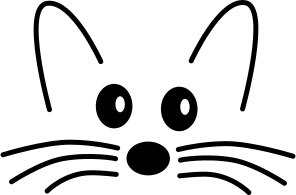
\includegraphics[width=1.4em]{squeak-logo}}}
\iftoshelse{
	\usepackage{marginnote}
		\renewcommand*{\marginfont}{\footnotesize}
	\newcommand{\vartriangleout}{\ifthenelse{\isodd{\thepage}}{\vartriangleright}{\vartriangleleft}}
	\newcommand{\dothisicon}{\fcolorbox{blue!65}{white}{\highlight{$\vartriangleout$}}}
	\newcommand{\dothis}[1]{%
		\noindent\par\noindent
		{\reversemarginpar
			\marginnote{\fcolorbox{blue!65}{white}{\highlight{$\vartriangleout$}}}}
		%\MarginLabel{do this}
		\noindent\emph{#1}
		\nopagebreak}
}{
	\newcommand{\dothisicon}{\raisebox{-.5ex}{
\includegraphics[height=1.2em]{pharo}}}
	\newcommand{\dothis}[1]{%
		\medskip
		\noindent\dothisicon
		\ifx#1\empty\else\quad\emph{#1}\fi
		\par\smallskip\nopagebreak}
}
%===> NEW VERSION <===
% NB: To use this in an individual chapter, you must set:
%\graphicspath{{figures/} {../figures/}}
% at the head of the chapter.  Don't forget the final /
%=============================================================
%:Reader hints (hint)
%
% Indicates a non-obvious consequence 
\newcommand{\hint}[1]{\vspace{1ex}\noindent\fbox{\textsc{Hint}} \emph{#1}}
%=================================================================
% graphics for Morphic handles
\newcommand{\grabHandle}{\raisebox{-0.2ex}{
\includegraphics[width=1em]{blackHandle}}}
\newcommand{\moveHandle}{\raisebox{-0.2ex}{
\includegraphics[width=1em]{moveHandle}}}
\newcommand{\debugHandle}{\raisebox{-0.2ex}{
\includegraphics[width=1em]{debugHandle}}}
%=============================================================
%:Highlighting Important stuff (doublebox)
%
% From Seaside book ...
\newsavebox{\SavedText}
\newlength{\InnerBoxRule}\setlength{\InnerBoxRule}{.75\fboxrule}
\newlength{\OuterBoxRule}\setlength{\OuterBoxRule}{1.5\fboxrule}
\newlength{\BoxSeparation}\setlength{\BoxSeparation}{1.5\fboxrule}
\addtolength{\BoxSeparation}{.5pt}
\newlength{\SaveBoxSep}\setlength{\SaveBoxSep}{2\fboxsep}
%
\newenvironment{doublebox}{\begin{lrbox}{\SavedText}
    \begin{minipage}{.75\textwidth}}
    {\end{minipage}\end{lrbox}\begin{center}
    \setlength{\fboxsep}{\BoxSeparation}\setlength{\fboxrule}{\OuterBoxRule}
    \fbox{\setlength{\fboxsep}{\SaveBoxSep}\setlength{\fboxrule}{\InnerBoxRule}%
      \fbox{\usebox{\SavedText}}}
  \end{center}}
% Use this:
\newcommand{\important}[1]{\begin{doublebox}#1\end{doublebox}}
%=============================================================
%:Section depth
\setcounter{secnumdepth}{2}
%% for this to happen start the file with
%\ifx\wholebook\relax\else
%% $Author$
% $Date$
% $Revision$

% HISTORY:
% 2006-10-31 - Oscar code macros
% ...

%=============================================================
% NB: documentclass must be set in main document.
% Allows book to be generated in multiple formats.
%=============================================================
%:Packages
\usepackage[T1]{fontenc}  %%%%%% really important to get the code directly in the text!
\usepackage{lmodern}
%\usepackage[scaled=0.85]{bookmanx} % needs another scale factor if used with \renewcommand{\sfdefault}{cmbr}
\usepackage{palatino}
\usepackage[scaled=0.85]{helvet}
\usepackage{microtype}
\usepackage{graphicx}
\usepackage{theorem}
\usepackage[english]{babel}
% ON: pdfsync breaks the use of p{width} for tabular columns!
\ifdefined\usepdfsync\usepackage{pdfsync}\fi % Requires texlive 2007
%=============================================================
%:More packages
%Stef should check which ones are used!
%\usepackage{picinpar}
%\usepackage{layout}
%\usepackage{color}
%\usepackage{enum}
%\usepackage{a4wide}
% \usepackage{fancyhdr}
\usepackage{ifthen}
\usepackage{float}
\usepackage{longtable}
\usepackage{makeidx}
\usepackage[nottoc]{tocbibind}
\usepackage{multicol}
\usepackage{booktabs}	% book-style tables
\usepackage{topcapt}	% enables \topcaption
\usepackage{multirow}
\usepackage{tabularx}
%\usepackage[bottom]{footmisc}
\usepackage{xspace}
\usepackage{alltt}
\usepackage{amssymb,textcomp}
\usepackage[usenames,dvipsnames]{color}
%\usepackage{colortbl}
\usepackage[hang]{subfigure}\makeatletter\def\p@subfigure{\thefigure\,}\makeatother
\usepackage{rotating}
\usepackage{enumitem}	% apb: allows more control over tags in enumerations
\usepackage{verbatim}     % for comment environment
\usepackage{varioref}	% for page references that work
\labelformat{footnote}{\thechapter--#1} % to distinguish citations from jurabib
\usepackage{needspace}
\usepackage{isodateo} % enable \isodate
\usepackage[newparttoc]{titlesec}
\usepackage{titletoc}
\usepackage{wrapfig}
\usepackage[
	super,
	citefull=first,
	authorformat={allreversed,and},
	titleformat={commasep,italic}
]{jurabib} % citations as footnotes
\usepackage[
	colorlinks=true,
	linkcolor=black,
	urlcolor=black,
	citecolor=black
]{hyperref}   % should come last
%=============================================================
%:PDF version
\pdfminorversion=3 % Set PDF to 1.3 for Lulu
%=============================================================
%:URL style
\makeatletter
\def\url@leostyle{%
  \@ifundefined{selectfont}{\def\UrlFont{\sf}}{\def\UrlFont{\sffamily}}}
\makeatother
% Now actually use the newly defined style.
\urlstyle{leo}
%=============================================================
%:Booleans
\newboolean{lulu}
\setboolean{lulu}{false}
\newcommand{\ifluluelse}[2]{\ifthenelse{\boolean{lulu}}{#1}{#2}}
%=============================================================
%:Names
\newcommand{\SUnit}{SUnit\xspace}
\newcommand{\sunit}{SUnit\xspace}
\newcommand{\xUnit}{$x$Unit\xspace}
\newcommand{\JUnit}{JUnit\xspace}
\newcommand{\st}{Smalltalk\xspace}
\newcommand{\pharo}{Pharo\xspace} % Use this, not \Pharo
%\newcommand{\sqmap}{SqueakMap\xspace}
\newcommand{\squeak}{Squeak\xspace} % use this, not \Squeak or \sq
\newcommand{\sqsrc}{SqueakSource\xspace}
\newcommand{\sbe}{\url{http://SqueakByExample.org}\xspace}
\newcommand{\pharoweb}{\url{http://pharo-project.org}\xspace}
\newcommand{\pbe}{\url{http://PharoByExample.org}\xspace}
\newcommand{\sba}{\url{http://SquareBracketAssociates.org}\xspace}
\newcommand{\bam}{\lct{Bounc\-ing\-Atoms\-Morph}\xspace}
%=============================================================
%:Markup macros for proof-reading
\usepackage[normalem]{ulem} % for \sout
\usepackage{xcolor}
\newcommand{\ra}{$\rightarrow$}
\newcommand{\ugh}[1]{\textcolor{red}{\uwave{#1}}} % please rephrase
\newcommand{\ins}[1]{\textcolor{blue}{\uline{#1}}} % please insert
\newcommand{\del}[1]{\textcolor{red}{\sout{#1}}} % please delete
\newcommand{\chg}[2]{\textcolor{red}{\sout{#1}}{\ra}\textcolor{blue}{\uline{#2}}} % please change
%=============================================================
%:Editorial comment macros
%\newcommand{\nnbb}[2]{
%    % \fbox{\bfseries\sffamily\scriptsize#1}
%    \fcolorbox{gray}{yellow}{\bfseries\sffamily\scriptsize#1}
%    {\sf\small$\blacktriangleright$\textit{#2}$\blacktriangleleft$}
%   }
\newcommand{\yellowbox}[1]{\fcolorbox{gray}{yellow}{\bfseries\sffamily\scriptsize#1}}
\newcommand{\triangles}[1]{{\sf\small$\blacktriangleright$\textit{#1}$\blacktriangleleft$}}
\newcommand{\nnbb}[2]{\yellowbox{#1} \triangles{#2}}
\newcommand{\fix}{\yellowbox{FIX!}}
\newcommand{\here}{\yellowbox{CONTINUE HERE!}}
% editor macros
\newcommand{\ab}[1]{\nnbb{Andrew}{#1}} % Black
\newcommand{\sd}[1]{\nnbb{St\'{e}f}{#1}} % Ducasse
\newcommand{\md}[1]{\nnbb{Marcus}{#1}} % Denker
\newcommand{\on}[1]{\nnbb{Oscar}{#1}} % Nierstrasz
\newcommand{\damien}[1]{\nnbb{Damien}{#1}} % Pollet
\newcommand{\lr}[1]{\nnbb{Lukas}{#1}} % Renggli
\newcommand{\orla}[1]{\nnbb{Orla}{#1}} % Greevy
\newcommand{\alex}[1]{\nnbb{Alex}{#1}} % Bergel
\newcommand{\alx}[1]{\nnbb{Alex}{#1}} % Bergel
\newcommand{\dr}[1]{\nnbb{David}{#1}} % Roethlisberger
\newcommand{\ja}[1]{\nnbb{Jannik}{#1}} % Laval
\newcommand{\jr}[1]{\nnbb{Jorge}{#1}} % Ressia
\newcommand{\fp}[1]{\nnbb{Fabrizio}{#1}} % Perin
\newcommand{\michael}[1]{\nnbb{Michael}{#1}} % Davies
\newcommand{\ew}[1]{\nnbb{Erwann}{#1}} % Wernli
\newcommand{\mb}[1]{\nnbb{Martial}{#1}} % Boniou
\newcommand{\hw}[1]{\nnbb{Hernan}{#1}} % Wilkinson
%=============================================================
%:Abbreviation macros
\newcommand{\ie}{\emph{i.e.},\xspace}
\newcommand{\eg}{\emph{e.g.},\xspace}
\newcommand{\etc}{etc.\xspace}
%=============================================================
%:Cross reference macros
\newcommand{\charef}[1]{Chapter~\ref{cha:#1}\xspace}
\newcommand{\secref}[1]{Section~\ref{sec:#1}\xspace}
\newcommand{\figref}[1]{Figure~\ref{fig:#1}\xspace}
\newcommand{\Figref}[1]{Figure~\ref{fig:#1}\xspace}
\newcommand{\appref}[1]{Appendix~\ref{app:#1}\xspace}
\newcommand{\tabref}[1]{Table~\ref{tab:#1}\xspace}
\newcommand{\faqref}[1]{FAQ~\ref{faq:#1}, p.~\pageref{faq:#1}\xspace}
% APB: I removed trailing \xspace commands from these macros because
% \xspace mostly doesn't work.  If you want a space after your
% references, type one!
% ON: xspace has always worked just fine for me!  Please leave them in.
%
\newcommand{\ruleref}[1]{\ref{rule:#1}\xspace}
%
\newcommand{\egref}[1]{example~\ref{eg:#1}\xspace}
\newcommand{\Egref}[1]{Example~\ref{eg:#1}\xspace}
%
\newcommand{\scrref}[1]{script~\ref{scr:#1}\xspace}
\newcommand{\Scrref}[1]{Script~\ref{scr:#1}\xspace}
\newcommand{\tscrref}[1]{the script~\ref{scr:#1}\xspace}
\newcommand{\Tscrref}[1]{The script~\ref{scr:#1}\xspace}
%
\newcommand{\mthref}[1]{method~\ref{mth:#1}\xspace}
\newcommand{\mthsref}[1]{methods~\ref{mth:#1}\xspace}
\newcommand{\Mthref}[1]{Method~\ref{mth:#1}\xspace}
\newcommand{\tmthref}[1]{the method~\ref{mth:#1}\xspace}
\newcommand{\Tmthref}[1]{The method~\ref{mth:#1}\xspace}
%
\newcommand{\clsref}[1]{class~\ref{cls:#1}\xspace}
\newcommand{\tclsref}[1]{the class~\ref{cls:#1}\xspace}
\newcommand{\Tclsref}[1]{The class~\ref{cls:#1}\xspace}

\newcommand{\chalabel}[1]{\label{cha:#1}}
\newcommand{\seclabel}[1]{\label{sec:#1}}
\newcommand{\figlabel}[1]{\label{fig:#1}}
\newcommand{\tablabel}[1]{\label{tab:#1}}
\newcommand{\rulelabel}[1]{\label{rule:#1}}
\newcommand{\eglabel}[1]{\label{eg:#1}}
\newcommand{\scrlabel}[1]{\label{scr:#1}}
\newcommand{\mthlabel}[1]{\label{mth:#1}}
\newcommand{\clslabel}[1]{\label{cls:#1}}
\newcommand{\faqlabel}[1]{\label{faq:#1}}
%=============================================================
%:Menu item macro
% for menu items, so we can change our minds on how to print them! (apb)
\definecolor{lightgray}{gray}{0.89}
\newcommand{\menu}[1]{{%
	\setlength{\fboxsep}{0pt}%
	\colorbox{lightgray}{{{\upshape\sffamily\strut \,#1\,}}}}}
\newcommand{\link}[1]{{%
	\fontfamily{lmr}\selectfont
 	\upshape{\sffamily \underline{#1}}}}
% For submenu items:
\newcommand{\go}{\,$\triangleright$\,}
% \newcommand{\go}{\,$\blacktriangleright$\,}
% For keyboard shortcuts:
%\newcommand{\short}[1]{\mbox{$\langle${\sc CMD}$\rangle$-#1}\xspace}
\newcommand{\short}[1]{\mbox{{\sc cmd}\hspace{0.08em}--\hspace{0.09em}#1}\xspace}
% For buttons:
\newcommand{\button}[1]{{%
	\setlength{\fboxsep}{0pt}%
	\fbox{{\upshape\sffamily\strut \,#1\,}}}}
% NB: The button macro does not work within captions -- incompatible with xcolor package :-(
\newcommand{\toolsflap}{\textit{Tools} flap\xspace}
%=============================================================
%:Mouse clicks
\newcommand{\click}{click\xspace} % RED
\newcommand{\actclick}{action-click\xspace} % YELLOW
\newcommand{\metaclick}{meta-click\xspace} % BLUE
\newcommand{\Click}{Click\xspace} % RED
\newcommand{\Actclick}{Action-click\xspace} % YELLOW
\newcommand{\Metaclick}{Meta-click\xspace} % BLUE
%=============================================================
%:ToSh macros
\newboolean{tosh}
\setboolean{tosh}{false}
\newcommand{\iftoshelse}[2]{\ifthenelse{\boolean{tosh}}{#1}{#2}}
%=============================================================
%:ToSh colors
%\newcommand{\highlightcolor}{\color{blue!65}}
%\newcommand{\boxcolor}{\color{gray!25}}
\newcommand{\highlight}[1]{\textcolor{blue!65}{#1}}
%\newcommand{\codecolor}{\color{blue!65}}
%%\setlength{\fboxrule}{2pt}
%\newcommand{\asPict}[1]{%
%	{\Large\highlight{#1}}}
%=============================================================
%:Reader cues (do this)
%
% Indicate something the reader should try out.
% \newcommand{\dothisicon}{\raisebox{-.5ex}{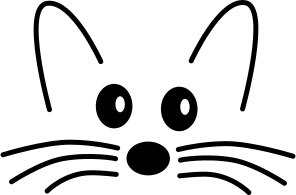
\includegraphics[width=1.4em]{squeak-logo}}}
\iftoshelse{
	\usepackage{marginnote}
		\renewcommand*{\marginfont}{\footnotesize}
	\newcommand{\vartriangleout}{\ifthenelse{\isodd{\thepage}}{\vartriangleright}{\vartriangleleft}}
	\newcommand{\dothisicon}{\fcolorbox{blue!65}{white}{\highlight{$\vartriangleout$}}}
	\newcommand{\dothis}[1]{%
		\noindent\par\noindent
		{\reversemarginpar
			\marginnote{\fcolorbox{blue!65}{white}{\highlight{$\vartriangleout$}}}}
		%\MarginLabel{do this}
		\noindent\emph{#1}
		\nopagebreak}
}{
	\newcommand{\dothisicon}{\raisebox{-.5ex}{
\includegraphics[height=1.2em]{pharo}}}
	\newcommand{\dothis}[1]{%
		\medskip
		\noindent\dothisicon
		\ifx#1\empty\else\quad\emph{#1}\fi
		\par\smallskip\nopagebreak}
}
%===> NEW VERSION <===
% NB: To use this in an individual chapter, you must set:
%\graphicspath{{figures/} {../figures/}}
% at the head of the chapter.  Don't forget the final /
%=============================================================
%:Reader hints (hint)
%
% Indicates a non-obvious consequence 
\newcommand{\hint}[1]{\vspace{1ex}\noindent\fbox{\textsc{Hint}} \emph{#1}}
%=================================================================
% graphics for Morphic handles
\newcommand{\grabHandle}{\raisebox{-0.2ex}{
\includegraphics[width=1em]{blackHandle}}}
\newcommand{\moveHandle}{\raisebox{-0.2ex}{
\includegraphics[width=1em]{moveHandle}}}
\newcommand{\debugHandle}{\raisebox{-0.2ex}{
\includegraphics[width=1em]{debugHandle}}}
%=============================================================
%:Highlighting Important stuff (doublebox)
%
% From Seaside book ...
\newsavebox{\SavedText}
\newlength{\InnerBoxRule}\setlength{\InnerBoxRule}{.75\fboxrule}
\newlength{\OuterBoxRule}\setlength{\OuterBoxRule}{1.5\fboxrule}
\newlength{\BoxSeparation}\setlength{\BoxSeparation}{1.5\fboxrule}
\addtolength{\BoxSeparation}{.5pt}
\newlength{\SaveBoxSep}\setlength{\SaveBoxSep}{2\fboxsep}
%
\newenvironment{doublebox}{\begin{lrbox}{\SavedText}
    \begin{minipage}{.75\textwidth}}
    {\end{minipage}\end{lrbox}\begin{center}
    \setlength{\fboxsep}{\BoxSeparation}\setlength{\fboxrule}{\OuterBoxRule}
    \fbox{\setlength{\fboxsep}{\SaveBoxSep}\setlength{\fboxrule}{\InnerBoxRule}%
      \fbox{\usebox{\SavedText}}}
  \end{center}}
% Use this:
\newcommand{\important}[1]{\begin{doublebox}#1\end{doublebox}}
%=============================================================
%:Section depth
\setcounter{secnumdepth}{2}
%% for this to happen start the file with
%\ifx\wholebook\relax\else
%% $Author$
% $Date$
% $Revision$

% HISTORY:
% 2006-10-31 - Oscar code macros
% ...

%=============================================================
% NB: documentclass must be set in main document.
% Allows book to be generated in multiple formats.
%=============================================================
%:Packages
\usepackage[T1]{fontenc}  %%%%%% really important to get the code directly in the text!
\usepackage{lmodern}
%\usepackage[scaled=0.85]{bookmanx} % needs another scale factor if used with \renewcommand{\sfdefault}{cmbr}
\usepackage{palatino}
\usepackage[scaled=0.85]{helvet}
\usepackage{microtype}
\usepackage{graphicx}
\usepackage{theorem}
\usepackage[english]{babel}
% ON: pdfsync breaks the use of p{width} for tabular columns!
\ifdefined\usepdfsync\usepackage{pdfsync}\fi % Requires texlive 2007
%=============================================================
%:More packages
%Stef should check which ones are used!
%\usepackage{picinpar}
%\usepackage{layout}
%\usepackage{color}
%\usepackage{enum}
%\usepackage{a4wide}
% \usepackage{fancyhdr}
\usepackage{ifthen}
\usepackage{float}
\usepackage{longtable}
\usepackage{makeidx}
\usepackage[nottoc]{tocbibind}
\usepackage{multicol}
\usepackage{booktabs}	% book-style tables
\usepackage{topcapt}	% enables \topcaption
\usepackage{multirow}
\usepackage{tabularx}
%\usepackage[bottom]{footmisc}
\usepackage{xspace}
\usepackage{alltt}
\usepackage{amssymb,textcomp}
\usepackage[usenames,dvipsnames]{color}
%\usepackage{colortbl}
\usepackage[hang]{subfigure}\makeatletter\def\p@subfigure{\thefigure\,}\makeatother
\usepackage{rotating}
\usepackage{enumitem}	% apb: allows more control over tags in enumerations
\usepackage{verbatim}     % for comment environment
\usepackage{varioref}	% for page references that work
\labelformat{footnote}{\thechapter--#1} % to distinguish citations from jurabib
\usepackage{needspace}
\usepackage{isodateo} % enable \isodate
\usepackage[newparttoc]{titlesec}
\usepackage{titletoc}
\usepackage{wrapfig}
\usepackage[
	super,
	citefull=first,
	authorformat={allreversed,and},
	titleformat={commasep,italic}
]{jurabib} % citations as footnotes
\usepackage[
	colorlinks=true,
	linkcolor=black,
	urlcolor=black,
	citecolor=black
]{hyperref}   % should come last
%=============================================================
%:PDF version
\pdfminorversion=3 % Set PDF to 1.3 for Lulu
%=============================================================
%:URL style
\makeatletter
\def\url@leostyle{%
  \@ifundefined{selectfont}{\def\UrlFont{\sf}}{\def\UrlFont{\sffamily}}}
\makeatother
% Now actually use the newly defined style.
\urlstyle{leo}
%=============================================================
%:Booleans
\newboolean{lulu}
\setboolean{lulu}{false}
\newcommand{\ifluluelse}[2]{\ifthenelse{\boolean{lulu}}{#1}{#2}}
%=============================================================
%:Names
\newcommand{\SUnit}{SUnit\xspace}
\newcommand{\sunit}{SUnit\xspace}
\newcommand{\xUnit}{$x$Unit\xspace}
\newcommand{\JUnit}{JUnit\xspace}
\newcommand{\st}{Smalltalk\xspace}
\newcommand{\pharo}{Pharo\xspace} % Use this, not \Pharo
%\newcommand{\sqmap}{SqueakMap\xspace}
\newcommand{\squeak}{Squeak\xspace} % use this, not \Squeak or \sq
\newcommand{\sqsrc}{SqueakSource\xspace}
\newcommand{\sbe}{\url{http://SqueakByExample.org}\xspace}
\newcommand{\pharoweb}{\url{http://pharo-project.org}\xspace}
\newcommand{\pbe}{\url{http://PharoByExample.org}\xspace}
\newcommand{\sba}{\url{http://SquareBracketAssociates.org}\xspace}
\newcommand{\bam}{\lct{Bounc\-ing\-Atoms\-Morph}\xspace}
%=============================================================
%:Markup macros for proof-reading
\usepackage[normalem]{ulem} % for \sout
\usepackage{xcolor}
\newcommand{\ra}{$\rightarrow$}
\newcommand{\ugh}[1]{\textcolor{red}{\uwave{#1}}} % please rephrase
\newcommand{\ins}[1]{\textcolor{blue}{\uline{#1}}} % please insert
\newcommand{\del}[1]{\textcolor{red}{\sout{#1}}} % please delete
\newcommand{\chg}[2]{\textcolor{red}{\sout{#1}}{\ra}\textcolor{blue}{\uline{#2}}} % please change
%=============================================================
%:Editorial comment macros
%\newcommand{\nnbb}[2]{
%    % \fbox{\bfseries\sffamily\scriptsize#1}
%    \fcolorbox{gray}{yellow}{\bfseries\sffamily\scriptsize#1}
%    {\sf\small$\blacktriangleright$\textit{#2}$\blacktriangleleft$}
%   }
\newcommand{\yellowbox}[1]{\fcolorbox{gray}{yellow}{\bfseries\sffamily\scriptsize#1}}
\newcommand{\triangles}[1]{{\sf\small$\blacktriangleright$\textit{#1}$\blacktriangleleft$}}
\newcommand{\nnbb}[2]{\yellowbox{#1} \triangles{#2}}
\newcommand{\fix}{\yellowbox{FIX!}}
\newcommand{\here}{\yellowbox{CONTINUE HERE!}}
% editor macros
\newcommand{\ab}[1]{\nnbb{Andrew}{#1}} % Black
\newcommand{\sd}[1]{\nnbb{St\'{e}f}{#1}} % Ducasse
\newcommand{\md}[1]{\nnbb{Marcus}{#1}} % Denker
\newcommand{\on}[1]{\nnbb{Oscar}{#1}} % Nierstrasz
\newcommand{\damien}[1]{\nnbb{Damien}{#1}} % Pollet
\newcommand{\lr}[1]{\nnbb{Lukas}{#1}} % Renggli
\newcommand{\orla}[1]{\nnbb{Orla}{#1}} % Greevy
\newcommand{\alex}[1]{\nnbb{Alex}{#1}} % Bergel
\newcommand{\alx}[1]{\nnbb{Alex}{#1}} % Bergel
\newcommand{\dr}[1]{\nnbb{David}{#1}} % Roethlisberger
\newcommand{\ja}[1]{\nnbb{Jannik}{#1}} % Laval
\newcommand{\jr}[1]{\nnbb{Jorge}{#1}} % Ressia
\newcommand{\fp}[1]{\nnbb{Fabrizio}{#1}} % Perin
\newcommand{\michael}[1]{\nnbb{Michael}{#1}} % Davies
\newcommand{\ew}[1]{\nnbb{Erwann}{#1}} % Wernli
\newcommand{\mb}[1]{\nnbb{Martial}{#1}} % Boniou
\newcommand{\hw}[1]{\nnbb{Hernan}{#1}} % Wilkinson
%=============================================================
%:Abbreviation macros
\newcommand{\ie}{\emph{i.e.},\xspace}
\newcommand{\eg}{\emph{e.g.},\xspace}
\newcommand{\etc}{etc.\xspace}
%=============================================================
%:Cross reference macros
\newcommand{\charef}[1]{Chapter~\ref{cha:#1}\xspace}
\newcommand{\secref}[1]{Section~\ref{sec:#1}\xspace}
\newcommand{\figref}[1]{Figure~\ref{fig:#1}\xspace}
\newcommand{\Figref}[1]{Figure~\ref{fig:#1}\xspace}
\newcommand{\appref}[1]{Appendix~\ref{app:#1}\xspace}
\newcommand{\tabref}[1]{Table~\ref{tab:#1}\xspace}
\newcommand{\faqref}[1]{FAQ~\ref{faq:#1}, p.~\pageref{faq:#1}\xspace}
% APB: I removed trailing \xspace commands from these macros because
% \xspace mostly doesn't work.  If you want a space after your
% references, type one!
% ON: xspace has always worked just fine for me!  Please leave them in.
%
\newcommand{\ruleref}[1]{\ref{rule:#1}\xspace}
%
\newcommand{\egref}[1]{example~\ref{eg:#1}\xspace}
\newcommand{\Egref}[1]{Example~\ref{eg:#1}\xspace}
%
\newcommand{\scrref}[1]{script~\ref{scr:#1}\xspace}
\newcommand{\Scrref}[1]{Script~\ref{scr:#1}\xspace}
\newcommand{\tscrref}[1]{the script~\ref{scr:#1}\xspace}
\newcommand{\Tscrref}[1]{The script~\ref{scr:#1}\xspace}
%
\newcommand{\mthref}[1]{method~\ref{mth:#1}\xspace}
\newcommand{\mthsref}[1]{methods~\ref{mth:#1}\xspace}
\newcommand{\Mthref}[1]{Method~\ref{mth:#1}\xspace}
\newcommand{\tmthref}[1]{the method~\ref{mth:#1}\xspace}
\newcommand{\Tmthref}[1]{The method~\ref{mth:#1}\xspace}
%
\newcommand{\clsref}[1]{class~\ref{cls:#1}\xspace}
\newcommand{\tclsref}[1]{the class~\ref{cls:#1}\xspace}
\newcommand{\Tclsref}[1]{The class~\ref{cls:#1}\xspace}

\newcommand{\chalabel}[1]{\label{cha:#1}}
\newcommand{\seclabel}[1]{\label{sec:#1}}
\newcommand{\figlabel}[1]{\label{fig:#1}}
\newcommand{\tablabel}[1]{\label{tab:#1}}
\newcommand{\rulelabel}[1]{\label{rule:#1}}
\newcommand{\eglabel}[1]{\label{eg:#1}}
\newcommand{\scrlabel}[1]{\label{scr:#1}}
\newcommand{\mthlabel}[1]{\label{mth:#1}}
\newcommand{\clslabel}[1]{\label{cls:#1}}
\newcommand{\faqlabel}[1]{\label{faq:#1}}
%=============================================================
%:Menu item macro
% for menu items, so we can change our minds on how to print them! (apb)
\definecolor{lightgray}{gray}{0.89}
\newcommand{\menu}[1]{{%
	\setlength{\fboxsep}{0pt}%
	\colorbox{lightgray}{{{\upshape\sffamily\strut \,#1\,}}}}}
\newcommand{\link}[1]{{%
	\fontfamily{lmr}\selectfont
 	\upshape{\sffamily \underline{#1}}}}
% For submenu items:
\newcommand{\go}{\,$\triangleright$\,}
% \newcommand{\go}{\,$\blacktriangleright$\,}
% For keyboard shortcuts:
%\newcommand{\short}[1]{\mbox{$\langle${\sc CMD}$\rangle$-#1}\xspace}
\newcommand{\short}[1]{\mbox{{\sc cmd}\hspace{0.08em}--\hspace{0.09em}#1}\xspace}
% For buttons:
\newcommand{\button}[1]{{%
	\setlength{\fboxsep}{0pt}%
	\fbox{{\upshape\sffamily\strut \,#1\,}}}}
% NB: The button macro does not work within captions -- incompatible with xcolor package :-(
\newcommand{\toolsflap}{\textit{Tools} flap\xspace}
%=============================================================
%:Mouse clicks
\newcommand{\click}{click\xspace} % RED
\newcommand{\actclick}{action-click\xspace} % YELLOW
\newcommand{\metaclick}{meta-click\xspace} % BLUE
\newcommand{\Click}{Click\xspace} % RED
\newcommand{\Actclick}{Action-click\xspace} % YELLOW
\newcommand{\Metaclick}{Meta-click\xspace} % BLUE
%=============================================================
%:ToSh macros
\newboolean{tosh}
\setboolean{tosh}{false}
\newcommand{\iftoshelse}[2]{\ifthenelse{\boolean{tosh}}{#1}{#2}}
%=============================================================
%:ToSh colors
%\newcommand{\highlightcolor}{\color{blue!65}}
%\newcommand{\boxcolor}{\color{gray!25}}
\newcommand{\highlight}[1]{\textcolor{blue!65}{#1}}
%\newcommand{\codecolor}{\color{blue!65}}
%%\setlength{\fboxrule}{2pt}
%\newcommand{\asPict}[1]{%
%	{\Large\highlight{#1}}}
%=============================================================
%:Reader cues (do this)
%
% Indicate something the reader should try out.
% \newcommand{\dothisicon}{\raisebox{-.5ex}{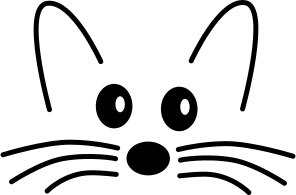
\includegraphics[width=1.4em]{squeak-logo}}}
\iftoshelse{
	\usepackage{marginnote}
		\renewcommand*{\marginfont}{\footnotesize}
	\newcommand{\vartriangleout}{\ifthenelse{\isodd{\thepage}}{\vartriangleright}{\vartriangleleft}}
	\newcommand{\dothisicon}{\fcolorbox{blue!65}{white}{\highlight{$\vartriangleout$}}}
	\newcommand{\dothis}[1]{%
		\noindent\par\noindent
		{\reversemarginpar
			\marginnote{\fcolorbox{blue!65}{white}{\highlight{$\vartriangleout$}}}}
		%\MarginLabel{do this}
		\noindent\emph{#1}
		\nopagebreak}
}{
	\newcommand{\dothisicon}{\raisebox{-.5ex}{
\includegraphics[height=1.2em]{pharo}}}
	\newcommand{\dothis}[1]{%
		\medskip
		\noindent\dothisicon
		\ifx#1\empty\else\quad\emph{#1}\fi
		\par\smallskip\nopagebreak}
}
%===> NEW VERSION <===
% NB: To use this in an individual chapter, you must set:
%\graphicspath{{figures/} {../figures/}}
% at the head of the chapter.  Don't forget the final /
%=============================================================
%:Reader hints (hint)
%
% Indicates a non-obvious consequence 
\newcommand{\hint}[1]{\vspace{1ex}\noindent\fbox{\textsc{Hint}} \emph{#1}}
%=================================================================
% graphics for Morphic handles
\newcommand{\grabHandle}{\raisebox{-0.2ex}{
\includegraphics[width=1em]{blackHandle}}}
\newcommand{\moveHandle}{\raisebox{-0.2ex}{
\includegraphics[width=1em]{moveHandle}}}
\newcommand{\debugHandle}{\raisebox{-0.2ex}{
\includegraphics[width=1em]{debugHandle}}}
%=============================================================
%:Highlighting Important stuff (doublebox)
%
% From Seaside book ...
\newsavebox{\SavedText}
\newlength{\InnerBoxRule}\setlength{\InnerBoxRule}{.75\fboxrule}
\newlength{\OuterBoxRule}\setlength{\OuterBoxRule}{1.5\fboxrule}
\newlength{\BoxSeparation}\setlength{\BoxSeparation}{1.5\fboxrule}
\addtolength{\BoxSeparation}{.5pt}
\newlength{\SaveBoxSep}\setlength{\SaveBoxSep}{2\fboxsep}
%
\newenvironment{doublebox}{\begin{lrbox}{\SavedText}
    \begin{minipage}{.75\textwidth}}
    {\end{minipage}\end{lrbox}\begin{center}
    \setlength{\fboxsep}{\BoxSeparation}\setlength{\fboxrule}{\OuterBoxRule}
    \fbox{\setlength{\fboxsep}{\SaveBoxSep}\setlength{\fboxrule}{\InnerBoxRule}%
      \fbox{\usebox{\SavedText}}}
  \end{center}}
% Use this:
\newcommand{\important}[1]{\begin{doublebox}#1\end{doublebox}}
%=============================================================
%:Section depth
\setcounter{secnumdepth}{2}
%% for this to happen start the file with
%\ifx\wholebook\relax\else
%\input{../common.tex}
%\begin{document}
%\fi
% and terminate by
% \ifx\wholebook\relax\else\end{document}\fi

\DeclareGraphicsExtensions{.pdf, .jpg, .png}
%=============================================================
%:PDF setup
\hypersetup{
%   a4paper,
%   pdfstartview=FitV,
%   colorlinks,
%   linkcolor=darkblue,
%   citecolor=darkblue,
   pdftitle={Pharo by Example},
   pdfauthor={Andrew P. Black, St\'ephane Ducasse,	Oscar Nierstrasz,
Damien Pollet},
   pdfkeywords={Smalltalk, Squeak, Object-Oriented Programming, OOP},
   pdfsubject={Computer Science}
}
%=============================================================
%:Page layout and appearance
%
% \renewcommand{\headrulewidth}{0pt}
\renewcommand{\chaptermark}[1]{\markboth{#1}{}}
\renewcommand{\sectionmark}[1]{\markright{\thesection\ #1}}
\renewpagestyle{plain}[\small\itshape]{%
	\setheadrule{0pt}%
	\sethead[][][]{}{}{}%
	\setfoot[][][]{}{}{}}
\renewpagestyle{headings}[\small\itshape]{%
	\setheadrule{0pt}%
	\setmarks{chapter}{section}%
	\sethead[\thepage][][\chaptertitle]{\sectiontitle}{}{\thepage}%
	\setfoot[][][]{}{}{}}
%=============================================================
%:Title section setup and TOC numbering depth
\setcounter{secnumdepth}{1}
\setcounter{tocdepth}{1}
\titleformat{\part}[display]{\centering}{\huge\partname\ \thepart}{1em}{\Huge\textbf}[]
\titleformat{\chapter}[display]{}{\huge\chaptertitlename\ \thechapter}{1em}{\Huge\raggedright\textbf}[]
\titlecontents{part}[3pc]{%
		\pagebreak[2]\addvspace{1em plus.4em minus.2em}%
		\leavevmode\large\bfseries}
	{\contentslabel{3pc}}{\hspace*{-3pc}}
	{}[\nopagebreak]
\titlecontents{chapter}[3pc]{%
		\pagebreak[0]\addvspace{1em plus.2em minus.2em}%
		\leavevmode\bfseries}
	{\contentslabel{3pc}}{}
	{\hfill\contentspage}[\nopagebreak]
\dottedcontents{section}[3pc]{}{3pc}{1pc}
\dottedcontents{subsection}[3pc]{}{0pc}{1pc}
% \dottedcontents{subsection}[4.5em]{}{0pt}{1pc}
% Make \cleardoublepage insert really blank pages http://www.tex.ac.uk/cgi-bin/texfaq2html?label=reallyblank
\let\origdoublepage\cleardoublepage
\newcommand{\clearemptydoublepage}{%
  \clearpage
  {\pagestyle{empty}\origdoublepage}}
\let\cleardoublepage\clearemptydoublepage % see http://www.tex.ac.uk/cgi-bin/texfaq2html?label=patch
%=============================================================
%:FAQ macros (for FAQ chapter)
\newtheorem{faq}{FAQ}
\newcommand{\answer}{\paragraph{Answer}\ }
%=============================================================
%:Listings package configuration
% \newcommand{\caret}{\makebox{\raisebox{0.4ex}{\footnotesize{$\wedge$}}}}
\newcommand{\caret}{\^\,}
\newcommand{\escape}{{\sf \textbackslash}}
\definecolor{source}{gray}{0.95}
\usepackage{listings}
\lstdefinelanguage{Smalltalk}{
%  morekeywords={self,super,true,false,nil,thisContext}, % This is overkill
  morestring=[d]',
  morecomment=[s]{"}{"},
  alsoletter={\#:},
  escapechar={!},
  literate=
    {BANG}{!}1
    {CARET}{\^}1
    {UNDERSCORE}{\_}1
    {\\st}{Smalltalk}9 % convenience -- in case \st occurs in code
    % {'}{{\textquotesingle}}1 % replaced by upquote=true in \lstset
    {_}{{$\leftarrow$}}1
    {>>>}{{\sep}}1
    {^}{{$\uparrow$}}1
    {~}{{$\sim$}}1
    {-}{{\textminus}}1 %{-}{\hspace{-0.13em}}{-}}1  % the goal is to make - the same width as +
    % {+}{\sf+}1 %{\raisebox{0.08ex}{+}}}1      % and to raise + off the baseline to match -
    {-->}{{\quad$\longrightarrow$\quad}}3
	, % Don't forget the comma at the end!
  tabsize=4
}[keywords,comments,strings]

\lstset{language=Smalltalk,
	basicstyle=\sffamily,
	keywordstyle=\color{black}\bfseries,
	% stringstyle=\ttfamily, % Ugly! do we really want this? -- on
	mathescape=true,
	showstringspaces=false,
	keepspaces=true,
	breaklines=true,
	breakautoindent=true,
	backgroundcolor=\color{source},
	lineskip={-1pt}, % Ugly hack
	upquote=true, % straight quote; requires textcomp package
	columns=fullflexible} % no fixed width fonts
% In-line code (literal)
% Normally use this for all in-line code:
\newcommand{\ct}{\lstinline[mathescape=false,backgroundcolor=\color{white},basicstyle={\sffamily\upshape}]}
% apb 2007.8.28 added the \upshape declaration to avoid getting italicized code in \dothis{ } sections.
% In-line code (latex enabled)
% Use this only in special situations where \ct does not work
% (within section headings ...):
\newcommand{\lct}[1]{{\textsf{\textup{#1}}}}
% Use these for system categories and protocols:
\newcommand{\scat}[1]{\emph{\textsf{#1}}\xspace}
\newcommand{\pkg}[1]{\emph{\textsf{#1}}\xspace}
\newcommand{\prot}[1]{\emph{\textsf{#1}}\xspace}
% Code environments
% NB: the arg is for tests
% Only code and example environments may be tests
\lstnewenvironment{code}[1]{%
	\lstset{%
		% frame=lines,
		frame=single,
		framerule=0pt,
		mathescape=false
	}
}{}
\def\ignoredollar#1{}
%=============================================================
%:Code environments (method, script ...)
% NB: the third arg is for tests
% Only code and example environments may be tests
\lstnewenvironment{example}[3][defaultlabel]{%
	\renewcommand{\lstlistingname}{Example}%
	\lstset{
		% frame=lines,
		frame=single,
		framerule=0pt,
		mathescape=false,
		caption={\emph{#2}},
		label={eg:#1}
	}
}{}
\lstnewenvironment{script}[2][defaultlabel]{%
\renewcommand{\lstlistingname}{Script}%
	\lstset{
		% frame=lines,
		frame=single,
		framerule=0pt,
		mathescape=false,
		name={Script},
		caption={\emph{#2}},
		label={scr:#1}
	}
}{}
\lstnewenvironment{method}[2][defaultlabel]{%
	\renewcommand{\lstlistingname}{Method}%
	\lstset{
		% frame=lines,
		frame=single,
		framerule=0pt,
		mathescape=false,
		name={Method},
		caption={\emph{#2}},
		label={mth:#1}
	}
}{}
\lstnewenvironment{methods}[2][defaultlabel]{% just for multiple methods at once
	\renewcommand{\lstlistingname}{Methods}%
	\lstset{
		% frame=lines,
		frame=single,
		framerule=0pt,
		mathescape=false,
		name={Method},
		caption={\emph{#2}},
		label={mth:#1}
	}
}{}
\lstnewenvironment{numMethod}[2][defaultlabel]{%
	\renewcommand{\lstlistingname}{Method}%
	\lstset{
		numbers=left,
		numberstyle={\tiny\sffamily},
		% frame=lines,
		frame=single,
		framerule=0pt,
		mathescape=false,
		name={Method},
		caption={\emph{#2}},
		label={mth:#1}
	}
}{}
\lstnewenvironment{classdef}[2][defaultlabel]{%
	\renewcommand{\lstlistingname}{Class}%
	\lstset{
		% frame=lines,
		frame=single,
		framerule=0pt,
		mathescape=false,
		name={Class},
		caption={\emph{#2}},
		label={cls:#1}
	}
}{}
%=============================================================
%:Reserving space
% Usually need one more line than the actual lines of code
\newcommand{\needlines}[1]{\Needspace{#1\baselineskip}}
%=============================================================
%:Indexing macros
% Macros ending with "ind" generate text as well as an index entry
% Macros ending with "index" *only* generate an index entry
\newcommand{\ind}[1]{\index{#1}#1\xspace} % plain text
\newcommand{\subind}[2]{\index{#1!#2}#2\xspace} % show #2, subindex under #1
\newcommand{\emphind}[1]{\index{#1}\emph{#1}\xspace} % emph #1
\newcommand{\emphsubind}[2]{\index{#1!#2}\emph{#2}\xspace} % show emph #2, subindex inder #1
\newcommand{\scatind}[1]{\index{#1@\textsf{#1} (category)}\scat{#1}} % category
\newcommand{\pkgind}[1]{\index{#1@\textsf{#1} (package)}\pkg{#1}} % package
\newcommand{\protind}[1]{\index{#1@\textsf{#1} (protocol)}\prot{#1}} % protocol
\newcommand{\clsind}[1]{\index{#1@\textsf{#1} (class)}\ct{#1}\xspace}
% \newcommand{\clsind}[1]{\index{#1!\#@(class)}\ct{#1}\xspace} % class
\newcommand{\clsindplural}[1]{\index{#1!\#@(class)}\ct{#1}s\xspace} % class
\newcommand{\cvind}[1]{\index{#1@\textsf{#1} (class variable)}\ct{#1}\xspace} % class var
\newcommand{\glbind}[1]{\index{#1@\textsf{#1} (global)}\ct{#1}\xspace} % global
\newcommand{\patind}[1]{\index{#1@#1 (pattern)}\ct{#1}\xspace} % pattern
\newcommand{\pvind}[1]{\index{#1@\textsf{#1} (pseudo variable)}\ct{#1}\xspace} % pseudo var
\newcommand{\clsmthind}[2]{\index{#1!#2@\ct{#2}}\ct{#1>>>#2}\xspace} % class + method name
\newcommand{\mthind}[2]{\index{#1!#2@\ct{#2}}\ct{#2}\xspace} % show method name only
\newcommand{\lmthind}[2]{\index{#1!#2@\ct{#2}}\lct{#2}\xspace} % show method name only
\newcommand{\cmind}[2]{\index{#1!#2@\ct{#2}}\ct{#1>>>#2}\xspace} % show class>>method
\newcommand{\lcmind}[2]{\index{#1!#2@\ct{#2}}\lct{#1>>>#2}\xspace} % show class>>method
\newcommand{\toolsflapind}{\index{Tools flap}\toolsflap} % index tools flap
% The following only generate an index entry:
% \newcommand{\clsindex}[1]{\index{#1@\textsf{#1} (class)}}
\newcommand{\clsindex}[1]{\index{#1!\#@(class)}} % class
\newcommand{\mthindex}[2]{\index{#1!#2@\ct{#2}}} % method
\newcommand{\cmindex}[2]{\index{#1!#2@\ct{#2}}} % class>>method
\newcommand{\cvindex}[1]{\index{#1@\textsf{#1} (class variable)}} % class var
\newcommand{\glbindex}[1]{\index{#1@\textsf{#1} (global)}}% global
\newcommand{\pvindex}[1]{\index{#1@\textsf{#1} (pseudo variable)}}% pseudo var
\newcommand{\seeindex}[2]{\index{#1|see{#2}}} % #1, see #2
\newcommand{\scatindex}[1]{\index{#1@\textsf{#1} (category)}} % category
\newcommand{\pkgindex}[1]{\index{#1@\textsf{#1} (package)}} % package
\newcommand{\protindex}[1]{\index{#1@\textsf{#1} (protocol)}} % protocol
% How can we have the main entry page numbers in bold yet not break the hyperlink?
\newcommand{\boldidx}[1]{{\bf #1}} % breaks hyperlink
%\newcommand{\indmain}[1]{\index{#1|boldidx}#1\xspace} % plain text, main entry
%\newcommand{\emphsubindmain}[2]{\index{#1!#2|boldidx}\emph{#2}\xspace} % subindex, main entry
%\newcommand{\subindmain}[2]{\index{#1!#2|boldidx}#2\xspace} % subindex, main entry
%\newcommand{\clsindmain}[1]{\index{#1@\textsf{#1} (class)|boldidx}\ct{#1}\xspace}
%\newcommand{\clsindmain}[1]{\index{#1!\#@(class)|boldidx}\ct{#1}\xspace} % class main
%\newcommand{\indexmain}[1]{\index{#1|boldidx}} % main index entry only
\newcommand{\indmain}[1]{\index{#1}#1\xspace} % The main index entry for this item
\newcommand{\emphsubindmain}[2]{\index{#1!#2}\emph{#2}\xspace} % subindex, main entry
\newcommand{\subindmain}[2]{\index{#1!#2}#2\xspace} % subindex, main entry
%\newcommand{\clsindmain}[1]{\index{#1@\textsf{#1} (class)}\ct{#1}\xspace}
\newcommand{\clsindmain}[1]{\index{#1!\#@(class)}\ct{#1}\xspace} % class main
\newcommand{\clsindexmain}[1]{\index{#1!\#@(class)}} % class main index only
\newcommand{\indexmain}[1]{\index{#1}} 
%=============================================================
%:Code macros
% some constants
\newcommand{\codesize}{\small}
\newcommand{\codefont}{\sffamily}
%\newcommand{\cat}[1]{\textit{In category #1}}%%To remove later
\newlength{\scriptindent}
\setlength{\scriptindent}{.3cm}
%% Method presentation constants
\newlength{\methodindent}
\newlength{\methodwordlength}
\newlength{\aftermethod}
\setlength{\methodindent}{0.2cm}
\settowidth{\methodwordlength}{\ M\'ethode\ }
%=============================================================
%:Smalltalk macros
%\newcommand{\sep}{{$\gg$}}
\newcommand{\sep}{\mbox{>>}}
\newcommand{\self}{\lct{self}\xspace}
\newcommand{\super}{\lct{super}\xspace}
\newcommand{\nil}{\lct{nil}\xspace}
%=============================================================
% be less conservative about float placement
% these commands are from http://www.tex.ac.uk/cgi-bin/texfaq2html?label=floats
\renewcommand{\topfraction}{.9}
\renewcommand{\bottomfraction}{.9}
\renewcommand{\textfraction}{.1}
\renewcommand{\floatpagefraction}{.85}
\renewcommand{\dbltopfraction}{.66}
\renewcommand{\dblfloatpagefraction}{.85}
\setcounter{topnumber}{9}
\setcounter{bottomnumber}{9}
\setcounter{totalnumber}{20}
\setcounter{dbltopnumber}{9}
%=============================================================
% apb doesn't like paragraphs to run in to each other without a break
\parskip 1ex
%=============================================================
%:Stuff to check, merge or deprecate
%\setlength{\marginparsep}{2mm}
%\renewcommand{\baselinestretch}{1.1}
%=============================================================

%\begin{document}
%\fi
% and terminate by
% \ifx\wholebook\relax\else\end{document}\fi

\DeclareGraphicsExtensions{.pdf, .jpg, .png}
%=============================================================
%:PDF setup
\hypersetup{
%   a4paper,
%   pdfstartview=FitV,
%   colorlinks,
%   linkcolor=darkblue,
%   citecolor=darkblue,
   pdftitle={Pharo by Example},
   pdfauthor={Andrew P. Black, St\'ephane Ducasse,	Oscar Nierstrasz,
Damien Pollet},
   pdfkeywords={Smalltalk, Squeak, Object-Oriented Programming, OOP},
   pdfsubject={Computer Science}
}
%=============================================================
%:Page layout and appearance
%
% \renewcommand{\headrulewidth}{0pt}
\renewcommand{\chaptermark}[1]{\markboth{#1}{}}
\renewcommand{\sectionmark}[1]{\markright{\thesection\ #1}}
\renewpagestyle{plain}[\small\itshape]{%
	\setheadrule{0pt}%
	\sethead[][][]{}{}{}%
	\setfoot[][][]{}{}{}}
\renewpagestyle{headings}[\small\itshape]{%
	\setheadrule{0pt}%
	\setmarks{chapter}{section}%
	\sethead[\thepage][][\chaptertitle]{\sectiontitle}{}{\thepage}%
	\setfoot[][][]{}{}{}}
%=============================================================
%:Title section setup and TOC numbering depth
\setcounter{secnumdepth}{1}
\setcounter{tocdepth}{1}
\titleformat{\part}[display]{\centering}{\huge\partname\ \thepart}{1em}{\Huge\textbf}[]
\titleformat{\chapter}[display]{}{\huge\chaptertitlename\ \thechapter}{1em}{\Huge\raggedright\textbf}[]
\titlecontents{part}[3pc]{%
		\pagebreak[2]\addvspace{1em plus.4em minus.2em}%
		\leavevmode\large\bfseries}
	{\contentslabel{3pc}}{\hspace*{-3pc}}
	{}[\nopagebreak]
\titlecontents{chapter}[3pc]{%
		\pagebreak[0]\addvspace{1em plus.2em minus.2em}%
		\leavevmode\bfseries}
	{\contentslabel{3pc}}{}
	{\hfill\contentspage}[\nopagebreak]
\dottedcontents{section}[3pc]{}{3pc}{1pc}
\dottedcontents{subsection}[3pc]{}{0pc}{1pc}
% \dottedcontents{subsection}[4.5em]{}{0pt}{1pc}
% Make \cleardoublepage insert really blank pages http://www.tex.ac.uk/cgi-bin/texfaq2html?label=reallyblank
\let\origdoublepage\cleardoublepage
\newcommand{\clearemptydoublepage}{%
  \clearpage
  {\pagestyle{empty}\origdoublepage}}
\let\cleardoublepage\clearemptydoublepage % see http://www.tex.ac.uk/cgi-bin/texfaq2html?label=patch
%=============================================================
%:FAQ macros (for FAQ chapter)
\newtheorem{faq}{FAQ}
\newcommand{\answer}{\paragraph{Answer}\ }
%=============================================================
%:Listings package configuration
% \newcommand{\caret}{\makebox{\raisebox{0.4ex}{\footnotesize{$\wedge$}}}}
\newcommand{\caret}{\^\,}
\newcommand{\escape}{{\sf \textbackslash}}
\definecolor{source}{gray}{0.95}
\usepackage{listings}
\lstdefinelanguage{Smalltalk}{
%  morekeywords={self,super,true,false,nil,thisContext}, % This is overkill
  morestring=[d]',
  morecomment=[s]{"}{"},
  alsoletter={\#:},
  escapechar={!},
  literate=
    {BANG}{!}1
    {CARET}{\^}1
    {UNDERSCORE}{\_}1
    {\\st}{Smalltalk}9 % convenience -- in case \st occurs in code
    % {'}{{\textquotesingle}}1 % replaced by upquote=true in \lstset
    {_}{{$\leftarrow$}}1
    {>>>}{{\sep}}1
    {^}{{$\uparrow$}}1
    {~}{{$\sim$}}1
    {-}{{\textminus}}1 %{-}{\hspace{-0.13em}}{-}}1  % the goal is to make - the same width as +
    % {+}{\sf+}1 %{\raisebox{0.08ex}{+}}}1      % and to raise + off the baseline to match -
    {-->}{{\quad$\longrightarrow$\quad}}3
	, % Don't forget the comma at the end!
  tabsize=4
}[keywords,comments,strings]

\lstset{language=Smalltalk,
	basicstyle=\sffamily,
	keywordstyle=\color{black}\bfseries,
	% stringstyle=\ttfamily, % Ugly! do we really want this? -- on
	mathescape=true,
	showstringspaces=false,
	keepspaces=true,
	breaklines=true,
	breakautoindent=true,
	backgroundcolor=\color{source},
	lineskip={-1pt}, % Ugly hack
	upquote=true, % straight quote; requires textcomp package
	columns=fullflexible} % no fixed width fonts
% In-line code (literal)
% Normally use this for all in-line code:
\newcommand{\ct}{\lstinline[mathescape=false,backgroundcolor=\color{white},basicstyle={\sffamily\upshape}]}
% apb 2007.8.28 added the \upshape declaration to avoid getting italicized code in \dothis{ } sections.
% In-line code (latex enabled)
% Use this only in special situations where \ct does not work
% (within section headings ...):
\newcommand{\lct}[1]{{\textsf{\textup{#1}}}}
% Use these for system categories and protocols:
\newcommand{\scat}[1]{\emph{\textsf{#1}}\xspace}
\newcommand{\pkg}[1]{\emph{\textsf{#1}}\xspace}
\newcommand{\prot}[1]{\emph{\textsf{#1}}\xspace}
% Code environments
% NB: the arg is for tests
% Only code and example environments may be tests
\lstnewenvironment{code}[1]{%
	\lstset{%
		% frame=lines,
		frame=single,
		framerule=0pt,
		mathescape=false
	}
}{}
\def\ignoredollar#1{}
%=============================================================
%:Code environments (method, script ...)
% NB: the third arg is for tests
% Only code and example environments may be tests
\lstnewenvironment{example}[3][defaultlabel]{%
	\renewcommand{\lstlistingname}{Example}%
	\lstset{
		% frame=lines,
		frame=single,
		framerule=0pt,
		mathescape=false,
		caption={\emph{#2}},
		label={eg:#1}
	}
}{}
\lstnewenvironment{script}[2][defaultlabel]{%
\renewcommand{\lstlistingname}{Script}%
	\lstset{
		% frame=lines,
		frame=single,
		framerule=0pt,
		mathescape=false,
		name={Script},
		caption={\emph{#2}},
		label={scr:#1}
	}
}{}
\lstnewenvironment{method}[2][defaultlabel]{%
	\renewcommand{\lstlistingname}{Method}%
	\lstset{
		% frame=lines,
		frame=single,
		framerule=0pt,
		mathescape=false,
		name={Method},
		caption={\emph{#2}},
		label={mth:#1}
	}
}{}
\lstnewenvironment{methods}[2][defaultlabel]{% just for multiple methods at once
	\renewcommand{\lstlistingname}{Methods}%
	\lstset{
		% frame=lines,
		frame=single,
		framerule=0pt,
		mathescape=false,
		name={Method},
		caption={\emph{#2}},
		label={mth:#1}
	}
}{}
\lstnewenvironment{numMethod}[2][defaultlabel]{%
	\renewcommand{\lstlistingname}{Method}%
	\lstset{
		numbers=left,
		numberstyle={\tiny\sffamily},
		% frame=lines,
		frame=single,
		framerule=0pt,
		mathescape=false,
		name={Method},
		caption={\emph{#2}},
		label={mth:#1}
	}
}{}
\lstnewenvironment{classdef}[2][defaultlabel]{%
	\renewcommand{\lstlistingname}{Class}%
	\lstset{
		% frame=lines,
		frame=single,
		framerule=0pt,
		mathescape=false,
		name={Class},
		caption={\emph{#2}},
		label={cls:#1}
	}
}{}
%=============================================================
%:Reserving space
% Usually need one more line than the actual lines of code
\newcommand{\needlines}[1]{\Needspace{#1\baselineskip}}
%=============================================================
%:Indexing macros
% Macros ending with "ind" generate text as well as an index entry
% Macros ending with "index" *only* generate an index entry
\newcommand{\ind}[1]{\index{#1}#1\xspace} % plain text
\newcommand{\subind}[2]{\index{#1!#2}#2\xspace} % show #2, subindex under #1
\newcommand{\emphind}[1]{\index{#1}\emph{#1}\xspace} % emph #1
\newcommand{\emphsubind}[2]{\index{#1!#2}\emph{#2}\xspace} % show emph #2, subindex inder #1
\newcommand{\scatind}[1]{\index{#1@\textsf{#1} (category)}\scat{#1}} % category
\newcommand{\pkgind}[1]{\index{#1@\textsf{#1} (package)}\pkg{#1}} % package
\newcommand{\protind}[1]{\index{#1@\textsf{#1} (protocol)}\prot{#1}} % protocol
\newcommand{\clsind}[1]{\index{#1@\textsf{#1} (class)}\ct{#1}\xspace}
% \newcommand{\clsind}[1]{\index{#1!\#@(class)}\ct{#1}\xspace} % class
\newcommand{\clsindplural}[1]{\index{#1!\#@(class)}\ct{#1}s\xspace} % class
\newcommand{\cvind}[1]{\index{#1@\textsf{#1} (class variable)}\ct{#1}\xspace} % class var
\newcommand{\glbind}[1]{\index{#1@\textsf{#1} (global)}\ct{#1}\xspace} % global
\newcommand{\patind}[1]{\index{#1@#1 (pattern)}\ct{#1}\xspace} % pattern
\newcommand{\pvind}[1]{\index{#1@\textsf{#1} (pseudo variable)}\ct{#1}\xspace} % pseudo var
\newcommand{\clsmthind}[2]{\index{#1!#2@\ct{#2}}\ct{#1>>>#2}\xspace} % class + method name
\newcommand{\mthind}[2]{\index{#1!#2@\ct{#2}}\ct{#2}\xspace} % show method name only
\newcommand{\lmthind}[2]{\index{#1!#2@\ct{#2}}\lct{#2}\xspace} % show method name only
\newcommand{\cmind}[2]{\index{#1!#2@\ct{#2}}\ct{#1>>>#2}\xspace} % show class>>method
\newcommand{\lcmind}[2]{\index{#1!#2@\ct{#2}}\lct{#1>>>#2}\xspace} % show class>>method
\newcommand{\toolsflapind}{\index{Tools flap}\toolsflap} % index tools flap
% The following only generate an index entry:
% \newcommand{\clsindex}[1]{\index{#1@\textsf{#1} (class)}}
\newcommand{\clsindex}[1]{\index{#1!\#@(class)}} % class
\newcommand{\mthindex}[2]{\index{#1!#2@\ct{#2}}} % method
\newcommand{\cmindex}[2]{\index{#1!#2@\ct{#2}}} % class>>method
\newcommand{\cvindex}[1]{\index{#1@\textsf{#1} (class variable)}} % class var
\newcommand{\glbindex}[1]{\index{#1@\textsf{#1} (global)}}% global
\newcommand{\pvindex}[1]{\index{#1@\textsf{#1} (pseudo variable)}}% pseudo var
\newcommand{\seeindex}[2]{\index{#1|see{#2}}} % #1, see #2
\newcommand{\scatindex}[1]{\index{#1@\textsf{#1} (category)}} % category
\newcommand{\pkgindex}[1]{\index{#1@\textsf{#1} (package)}} % package
\newcommand{\protindex}[1]{\index{#1@\textsf{#1} (protocol)}} % protocol
% How can we have the main entry page numbers in bold yet not break the hyperlink?
\newcommand{\boldidx}[1]{{\bf #1}} % breaks hyperlink
%\newcommand{\indmain}[1]{\index{#1|boldidx}#1\xspace} % plain text, main entry
%\newcommand{\emphsubindmain}[2]{\index{#1!#2|boldidx}\emph{#2}\xspace} % subindex, main entry
%\newcommand{\subindmain}[2]{\index{#1!#2|boldidx}#2\xspace} % subindex, main entry
%\newcommand{\clsindmain}[1]{\index{#1@\textsf{#1} (class)|boldidx}\ct{#1}\xspace}
%\newcommand{\clsindmain}[1]{\index{#1!\#@(class)|boldidx}\ct{#1}\xspace} % class main
%\newcommand{\indexmain}[1]{\index{#1|boldidx}} % main index entry only
\newcommand{\indmain}[1]{\index{#1}#1\xspace} % The main index entry for this item
\newcommand{\emphsubindmain}[2]{\index{#1!#2}\emph{#2}\xspace} % subindex, main entry
\newcommand{\subindmain}[2]{\index{#1!#2}#2\xspace} % subindex, main entry
%\newcommand{\clsindmain}[1]{\index{#1@\textsf{#1} (class)}\ct{#1}\xspace}
\newcommand{\clsindmain}[1]{\index{#1!\#@(class)}\ct{#1}\xspace} % class main
\newcommand{\clsindexmain}[1]{\index{#1!\#@(class)}} % class main index only
\newcommand{\indexmain}[1]{\index{#1}} 
%=============================================================
%:Code macros
% some constants
\newcommand{\codesize}{\small}
\newcommand{\codefont}{\sffamily}
%\newcommand{\cat}[1]{\textit{In category #1}}%%To remove later
\newlength{\scriptindent}
\setlength{\scriptindent}{.3cm}
%% Method presentation constants
\newlength{\methodindent}
\newlength{\methodwordlength}
\newlength{\aftermethod}
\setlength{\methodindent}{0.2cm}
\settowidth{\methodwordlength}{\ M\'ethode\ }
%=============================================================
%:Smalltalk macros
%\newcommand{\sep}{{$\gg$}}
\newcommand{\sep}{\mbox{>>}}
\newcommand{\self}{\lct{self}\xspace}
\newcommand{\super}{\lct{super}\xspace}
\newcommand{\nil}{\lct{nil}\xspace}
%=============================================================
% be less conservative about float placement
% these commands are from http://www.tex.ac.uk/cgi-bin/texfaq2html?label=floats
\renewcommand{\topfraction}{.9}
\renewcommand{\bottomfraction}{.9}
\renewcommand{\textfraction}{.1}
\renewcommand{\floatpagefraction}{.85}
\renewcommand{\dbltopfraction}{.66}
\renewcommand{\dblfloatpagefraction}{.85}
\setcounter{topnumber}{9}
\setcounter{bottomnumber}{9}
\setcounter{totalnumber}{20}
\setcounter{dbltopnumber}{9}
%=============================================================
% apb doesn't like paragraphs to run in to each other without a break
\parskip 1ex
%=============================================================
%:Stuff to check, merge or deprecate
%\setlength{\marginparsep}{2mm}
%\renewcommand{\baselinestretch}{1.1}
%=============================================================

%\begin{document}
%\fi
% and terminate by
% \ifx\wholebook\relax\else\end{document}\fi

\DeclareGraphicsExtensions{.pdf, .jpg, .png}
%=============================================================
%:PDF setup
\hypersetup{
%   a4paper,
%   pdfstartview=FitV,
%   colorlinks,
%   linkcolor=darkblue,
%   citecolor=darkblue,
   pdftitle={Pharo by Example},
   pdfauthor={Andrew P. Black, St\'ephane Ducasse,	Oscar Nierstrasz,
Damien Pollet},
   pdfkeywords={Smalltalk, Squeak, Object-Oriented Programming, OOP},
   pdfsubject={Computer Science}
}
%=============================================================
%:Page layout and appearance
%
% \renewcommand{\headrulewidth}{0pt}
\renewcommand{\chaptermark}[1]{\markboth{#1}{}}
\renewcommand{\sectionmark}[1]{\markright{\thesection\ #1}}
\renewpagestyle{plain}[\small\itshape]{%
	\setheadrule{0pt}%
	\sethead[][][]{}{}{}%
	\setfoot[][][]{}{}{}}
\renewpagestyle{headings}[\small\itshape]{%
	\setheadrule{0pt}%
	\setmarks{chapter}{section}%
	\sethead[\thepage][][\chaptertitle]{\sectiontitle}{}{\thepage}%
	\setfoot[][][]{}{}{}}
%=============================================================
%:Title section setup and TOC numbering depth
\setcounter{secnumdepth}{1}
\setcounter{tocdepth}{1}
\titleformat{\part}[display]{\centering}{\huge\partname\ \thepart}{1em}{\Huge\textbf}[]
\titleformat{\chapter}[display]{}{\huge\chaptertitlename\ \thechapter}{1em}{\Huge\raggedright\textbf}[]
\titlecontents{part}[3pc]{%
		\pagebreak[2]\addvspace{1em plus.4em minus.2em}%
		\leavevmode\large\bfseries}
	{\contentslabel{3pc}}{\hspace*{-3pc}}
	{}[\nopagebreak]
\titlecontents{chapter}[3pc]{%
		\pagebreak[0]\addvspace{1em plus.2em minus.2em}%
		\leavevmode\bfseries}
	{\contentslabel{3pc}}{}
	{\hfill\contentspage}[\nopagebreak]
\dottedcontents{section}[3pc]{}{3pc}{1pc}
\dottedcontents{subsection}[3pc]{}{0pc}{1pc}
% \dottedcontents{subsection}[4.5em]{}{0pt}{1pc}
% Make \cleardoublepage insert really blank pages http://www.tex.ac.uk/cgi-bin/texfaq2html?label=reallyblank
\let\origdoublepage\cleardoublepage
\newcommand{\clearemptydoublepage}{%
  \clearpage
  {\pagestyle{empty}\origdoublepage}}
\let\cleardoublepage\clearemptydoublepage % see http://www.tex.ac.uk/cgi-bin/texfaq2html?label=patch
%=============================================================
%:FAQ macros (for FAQ chapter)
\newtheorem{faq}{FAQ}
\newcommand{\answer}{\paragraph{Answer}\ }
%=============================================================
%:Listings package configuration
% \newcommand{\caret}{\makebox{\raisebox{0.4ex}{\footnotesize{$\wedge$}}}}
\newcommand{\caret}{\^\,}
\newcommand{\escape}{{\sf \textbackslash}}
\definecolor{source}{gray}{0.95}
\usepackage{listings}
\lstdefinelanguage{Smalltalk}{
%  morekeywords={self,super,true,false,nil,thisContext}, % This is overkill
  morestring=[d]',
  morecomment=[s]{"}{"},
  alsoletter={\#:},
  escapechar={!},
  literate=
    {BANG}{!}1
    {CARET}{\^}1
    {UNDERSCORE}{\_}1
    {\\st}{Smalltalk}9 % convenience -- in case \st occurs in code
    % {'}{{\textquotesingle}}1 % replaced by upquote=true in \lstset
    {_}{{$\leftarrow$}}1
    {>>>}{{\sep}}1
    {^}{{$\uparrow$}}1
    {~}{{$\sim$}}1
    {-}{{\textminus}}1 %{-}{\hspace{-0.13em}}{-}}1  % the goal is to make - the same width as +
    % {+}{\sf+}1 %{\raisebox{0.08ex}{+}}}1      % and to raise + off the baseline to match -
    {-->}{{\quad$\longrightarrow$\quad}}3
	, % Don't forget the comma at the end!
  tabsize=4
}[keywords,comments,strings]

\lstset{language=Smalltalk,
	basicstyle=\sffamily,
	keywordstyle=\color{black}\bfseries,
	% stringstyle=\ttfamily, % Ugly! do we really want this? -- on
	mathescape=true,
	showstringspaces=false,
	keepspaces=true,
	breaklines=true,
	breakautoindent=true,
	backgroundcolor=\color{source},
	lineskip={-1pt}, % Ugly hack
	upquote=true, % straight quote; requires textcomp package
	columns=fullflexible} % no fixed width fonts
% In-line code (literal)
% Normally use this for all in-line code:
\newcommand{\ct}{\lstinline[mathescape=false,backgroundcolor=\color{white},basicstyle={\sffamily\upshape}]}
% apb 2007.8.28 added the \upshape declaration to avoid getting italicized code in \dothis{ } sections.
% In-line code (latex enabled)
% Use this only in special situations where \ct does not work
% (within section headings ...):
\newcommand{\lct}[1]{{\textsf{\textup{#1}}}}
% Use these for system categories and protocols:
\newcommand{\scat}[1]{\emph{\textsf{#1}}\xspace}
\newcommand{\pkg}[1]{\emph{\textsf{#1}}\xspace}
\newcommand{\prot}[1]{\emph{\textsf{#1}}\xspace}
% Code environments
% NB: the arg is for tests
% Only code and example environments may be tests
\lstnewenvironment{code}[1]{%
	\lstset{%
		% frame=lines,
		frame=single,
		framerule=0pt,
		mathescape=false
	}
}{}
\def\ignoredollar#1{}
%=============================================================
%:Code environments (method, script ...)
% NB: the third arg is for tests
% Only code and example environments may be tests
\lstnewenvironment{example}[3][defaultlabel]{%
	\renewcommand{\lstlistingname}{Example}%
	\lstset{
		% frame=lines,
		frame=single,
		framerule=0pt,
		mathescape=false,
		caption={\emph{#2}},
		label={eg:#1}
	}
}{}
\lstnewenvironment{script}[2][defaultlabel]{%
\renewcommand{\lstlistingname}{Script}%
	\lstset{
		% frame=lines,
		frame=single,
		framerule=0pt,
		mathescape=false,
		name={Script},
		caption={\emph{#2}},
		label={scr:#1}
	}
}{}
\lstnewenvironment{method}[2][defaultlabel]{%
	\renewcommand{\lstlistingname}{Method}%
	\lstset{
		% frame=lines,
		frame=single,
		framerule=0pt,
		mathescape=false,
		name={Method},
		caption={\emph{#2}},
		label={mth:#1}
	}
}{}
\lstnewenvironment{methods}[2][defaultlabel]{% just for multiple methods at once
	\renewcommand{\lstlistingname}{Methods}%
	\lstset{
		% frame=lines,
		frame=single,
		framerule=0pt,
		mathescape=false,
		name={Method},
		caption={\emph{#2}},
		label={mth:#1}
	}
}{}
\lstnewenvironment{numMethod}[2][defaultlabel]{%
	\renewcommand{\lstlistingname}{Method}%
	\lstset{
		numbers=left,
		numberstyle={\tiny\sffamily},
		% frame=lines,
		frame=single,
		framerule=0pt,
		mathescape=false,
		name={Method},
		caption={\emph{#2}},
		label={mth:#1}
	}
}{}
\lstnewenvironment{classdef}[2][defaultlabel]{%
	\renewcommand{\lstlistingname}{Class}%
	\lstset{
		% frame=lines,
		frame=single,
		framerule=0pt,
		mathescape=false,
		name={Class},
		caption={\emph{#2}},
		label={cls:#1}
	}
}{}
%=============================================================
%:Reserving space
% Usually need one more line than the actual lines of code
\newcommand{\needlines}[1]{\Needspace{#1\baselineskip}}
%=============================================================
%:Indexing macros
% Macros ending with "ind" generate text as well as an index entry
% Macros ending with "index" *only* generate an index entry
\newcommand{\ind}[1]{\index{#1}#1\xspace} % plain text
\newcommand{\subind}[2]{\index{#1!#2}#2\xspace} % show #2, subindex under #1
\newcommand{\emphind}[1]{\index{#1}\emph{#1}\xspace} % emph #1
\newcommand{\emphsubind}[2]{\index{#1!#2}\emph{#2}\xspace} % show emph #2, subindex inder #1
\newcommand{\scatind}[1]{\index{#1@\textsf{#1} (category)}\scat{#1}} % category
\newcommand{\pkgind}[1]{\index{#1@\textsf{#1} (package)}\pkg{#1}} % package
\newcommand{\protind}[1]{\index{#1@\textsf{#1} (protocol)}\prot{#1}} % protocol
\newcommand{\clsind}[1]{\index{#1@\textsf{#1} (class)}\ct{#1}\xspace}
% \newcommand{\clsind}[1]{\index{#1!\#@(class)}\ct{#1}\xspace} % class
\newcommand{\clsindplural}[1]{\index{#1!\#@(class)}\ct{#1}s\xspace} % class
\newcommand{\cvind}[1]{\index{#1@\textsf{#1} (class variable)}\ct{#1}\xspace} % class var
\newcommand{\glbind}[1]{\index{#1@\textsf{#1} (global)}\ct{#1}\xspace} % global
\newcommand{\patind}[1]{\index{#1@#1 (pattern)}\ct{#1}\xspace} % pattern
\newcommand{\pvind}[1]{\index{#1@\textsf{#1} (pseudo variable)}\ct{#1}\xspace} % pseudo var
\newcommand{\clsmthind}[2]{\index{#1!#2@\ct{#2}}\ct{#1>>>#2}\xspace} % class + method name
\newcommand{\mthind}[2]{\index{#1!#2@\ct{#2}}\ct{#2}\xspace} % show method name only
\newcommand{\lmthind}[2]{\index{#1!#2@\ct{#2}}\lct{#2}\xspace} % show method name only
\newcommand{\cmind}[2]{\index{#1!#2@\ct{#2}}\ct{#1>>>#2}\xspace} % show class>>method
\newcommand{\lcmind}[2]{\index{#1!#2@\ct{#2}}\lct{#1>>>#2}\xspace} % show class>>method
\newcommand{\toolsflapind}{\index{Tools flap}\toolsflap} % index tools flap
% The following only generate an index entry:
% \newcommand{\clsindex}[1]{\index{#1@\textsf{#1} (class)}}
\newcommand{\clsindex}[1]{\index{#1!\#@(class)}} % class
\newcommand{\mthindex}[2]{\index{#1!#2@\ct{#2}}} % method
\newcommand{\cmindex}[2]{\index{#1!#2@\ct{#2}}} % class>>method
\newcommand{\cvindex}[1]{\index{#1@\textsf{#1} (class variable)}} % class var
\newcommand{\glbindex}[1]{\index{#1@\textsf{#1} (global)}}% global
\newcommand{\pvindex}[1]{\index{#1@\textsf{#1} (pseudo variable)}}% pseudo var
\newcommand{\seeindex}[2]{\index{#1|see{#2}}} % #1, see #2
\newcommand{\scatindex}[1]{\index{#1@\textsf{#1} (category)}} % category
\newcommand{\pkgindex}[1]{\index{#1@\textsf{#1} (package)}} % package
\newcommand{\protindex}[1]{\index{#1@\textsf{#1} (protocol)}} % protocol
% How can we have the main entry page numbers in bold yet not break the hyperlink?
\newcommand{\boldidx}[1]{{\bf #1}} % breaks hyperlink
%\newcommand{\indmain}[1]{\index{#1|boldidx}#1\xspace} % plain text, main entry
%\newcommand{\emphsubindmain}[2]{\index{#1!#2|boldidx}\emph{#2}\xspace} % subindex, main entry
%\newcommand{\subindmain}[2]{\index{#1!#2|boldidx}#2\xspace} % subindex, main entry
%\newcommand{\clsindmain}[1]{\index{#1@\textsf{#1} (class)|boldidx}\ct{#1}\xspace}
%\newcommand{\clsindmain}[1]{\index{#1!\#@(class)|boldidx}\ct{#1}\xspace} % class main
%\newcommand{\indexmain}[1]{\index{#1|boldidx}} % main index entry only
\newcommand{\indmain}[1]{\index{#1}#1\xspace} % The main index entry for this item
\newcommand{\emphsubindmain}[2]{\index{#1!#2}\emph{#2}\xspace} % subindex, main entry
\newcommand{\subindmain}[2]{\index{#1!#2}#2\xspace} % subindex, main entry
%\newcommand{\clsindmain}[1]{\index{#1@\textsf{#1} (class)}\ct{#1}\xspace}
\newcommand{\clsindmain}[1]{\index{#1!\#@(class)}\ct{#1}\xspace} % class main
\newcommand{\clsindexmain}[1]{\index{#1!\#@(class)}} % class main index only
\newcommand{\indexmain}[1]{\index{#1}} 
%=============================================================
%:Code macros
% some constants
\newcommand{\codesize}{\small}
\newcommand{\codefont}{\sffamily}
%\newcommand{\cat}[1]{\textit{In category #1}}%%To remove later
\newlength{\scriptindent}
\setlength{\scriptindent}{.3cm}
%% Method presentation constants
\newlength{\methodindent}
\newlength{\methodwordlength}
\newlength{\aftermethod}
\setlength{\methodindent}{0.2cm}
\settowidth{\methodwordlength}{\ M\'ethode\ }
%=============================================================
%:Smalltalk macros
%\newcommand{\sep}{{$\gg$}}
\newcommand{\sep}{\mbox{>>}}
\newcommand{\self}{\lct{self}\xspace}
\newcommand{\super}{\lct{super}\xspace}
\newcommand{\nil}{\lct{nil}\xspace}
%=============================================================
% be less conservative about float placement
% these commands are from http://www.tex.ac.uk/cgi-bin/texfaq2html?label=floats
\renewcommand{\topfraction}{.9}
\renewcommand{\bottomfraction}{.9}
\renewcommand{\textfraction}{.1}
\renewcommand{\floatpagefraction}{.85}
\renewcommand{\dbltopfraction}{.66}
\renewcommand{\dblfloatpagefraction}{.85}
\setcounter{topnumber}{9}
\setcounter{bottomnumber}{9}
\setcounter{totalnumber}{20}
\setcounter{dbltopnumber}{9}
%=============================================================
% apb doesn't like paragraphs to run in to each other without a break
\parskip 1ex
%=============================================================
%:Stuff to check, merge or deprecate
%\setlength{\marginparsep}{2mm}
%\renewcommand{\baselinestretch}{1.1}
%=============================================================

%	\usepackage{a4wide}
% --------------------------------------------
    \graphicspath{{figures/} {../figures/}}
	\begin{document}
	% \renewcommand{\nnbb}[2]{} % Disable editorial comments
	\sloppy
\fi
%=================================================================
\chapter{El entorno de progamaci\'on Pharo}
\chalabel{env}


El objetivo de este capitulo es mostrar la forma de desarrollar programas en el entorno de programaci\'on \pharo.
Ya se ha visto como definir m\'etodos y clases usando el buscador; este capitulo mostrar\'a m\'as caracteristicas del buscador, e introducir\'a algunos de los dem\'as buscadores.

Por supuesto, ocasionalmente puede suceder que el programa no realice la funci\'on que de \'el se espera. Por ello, \pharo tiene un excelente depurador, pero al igual que otras herramientas poderosas, puede resultar confuso cuando se lo usa por primera vez. En este capitulo se dar\'a un ejemplo de depuraci\'on y se demostrar\'an algunas de las caracter\'isticas de esta herramienta.

Una de las caracter\'isticas \'unicas de Smalltalk es que mientras se est\'a programando, uno pertenece a un mundo de objetos vivos, muy distinto al de los programas est\'aticos. Esto hace posible obtener feedback de forma instantanea mientras se programa, lo cual permite al programador ser m\'as productivo. Hay dos herramientas que permiten analizar, e incluso cambiar, los objetos vivos: el \emph{inspector} y el \emph{explorer}.

La consecuencia de programar en un mundo de objetos vivos, en vez de hacerlo con archivos y un editor de texto, es que se debe realizar una acci\'on explicita para exportar el programa desde la imagen de Smalltalk.
La forma antigua de hacerlo, posible en todos los dialectos Smalltalk, es mediante crear un \emph{fileout} o un \emph{change set}, los cuales son en esencia archivos de texto encriptados que pueden ser importados desde otro sistema.
En cambio, la nueva forma de hacer esto en \pharo is subir el c\'odigo a un repositorio de versiones en un servidor.  Esto se logra usando una herramienta llamada \ind{Monticello}, y es una manera m\'as poderosa y eficiente de trabajar, especialmente en grupo.
\seeindex{change set}{file, filing out}
\index{file!filing out}

%Finally, you may find a bug in \pharo as you work; we explain how to report bugs, and how to submit bug fixes.
%\ab{Or I would, if I knew how.   We should do this, or remove the paragraph.}

%=========================================================
\section{Resumen}
\seclabel{overview}

Smalltalk y las interfaces gr\'aficas modernas fueron desarrolladas juntas.
Aun antes del primer lanzamiento p\'ublico de Smalltalk en 1983, este ten\'ia un entorno gr\'afico de desarrollo auto-alojado, y todo el desarrollo en Smalltalk tomaba lugar en \'el.
Para empezar, se ver\'an las herramientas principales de \pharo.

\begin{itemize}
	\item {El \menu{Browser}} es la principal herramienta de desarrollo. Se usa para crear, definir y organizar las clases y m\'etodos. Usandolo tambien se puede navegar por todas las librer\'ias de clase: a diferencia de otros entornos donde el c\'odigo fuente es almacenado en archivos diferentes, en Smalltalk todas las clases y m\'etodos est\'an contenidos en la imagen.
	\index{browser}

	\item{\menu{Message Names}} se usa para ver todos los m\'etodos con un selector particular, o con uno que contenga una subcadena de caracteres.
	\index{message name finder}
	
	\item{El \menu{Method Finder}} tambi\'en le ayudará a encontr\'ar m\'etodos, pero de acuerdo a lo que \emph{hacen} adem\'as de por su nombre.
	\index{method finder}
	
	\item{El \menu{Monticello Browser}} es el punto de partida para cargar c\'odigo desde, o guardar c\'odigo en, los paquetes \ind{Monticello}.

	\item{El \menu{Process Browser} permite ver todos los procesos (\emph{threads}) que se est\'an ejecutando en Smalltalk.}
	\index{process browser}
	
	\item{El \menu{Test Runner}} le permite correr y debbugear las pruebas \SUnit, y se describe en \charef{SUnit}.
	\index{Test Runner}
	\index{SUnit}
	
	\item{El \menu{Transcript}} es una ventana en el canal de salida del \glbind{Transcript}, el cual es \'util para escribir mensajes de registro y que ya se ha descripto en \secref{transcript}.
	
	\item{El \menu{Workspace}} es una ventana donde se pueden tipear entradas.
	Puede ser usado con cualquier propósito, pero es m\'as usado para tipear expresiones de Smalltalk y
	ejecutarlas con \menu{do it}. El uso del \ind{workspace} tambi\'en fue ilustrado en \secref{transcript}.

\end{itemize}

El \menu{Debugger} tiene una tarea obvia, pero descubrir\'a que tiene un rol más importante comparado con los debuggers de otros lenguajes de programaci\'on , porque en Smalltalk se puede \emph{programar} en el \ind{debugger}. El debugger no se lanza desde un men\'u; normalmente aparece al correr una prueba que falla, al tipear \short{\textbf{.}} para interrumpir un proceso en curso, o insertando una expreci\'on \ct{self halt} en el c\'odigo.
\index{process!interrupting}

%=========================================================
\section{El Navegador}
\seclabel{browser}

Muchos navegadores de clases diferentes se han desarrollado a trevez de los años para \st.
\pharo simplifica esta historia por medio de ofrecer un navegados que integra diversas vistas.
\figref{SystemBrowser0} muestra el navegador como aparece la primera vez que es abierto.\footnote{Recuerde que si el navegador que usted tenga no se ve como el mostrado en \figref{classBrowser}, quiz\'as necesite cambiar el navegador por defecto.  V\'ease \faqref{packagebrowser}.}

\begin{figure}[htbp]
   \centering
   \ifluluelse
	 {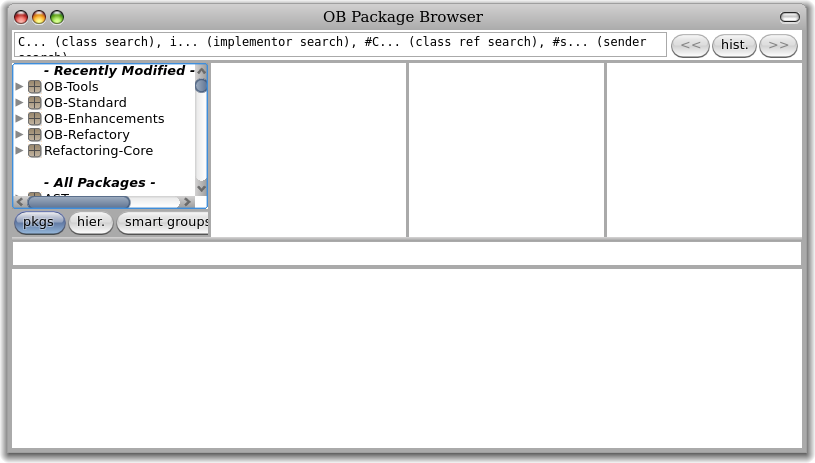
\includegraphics[width=\textwidth]{SystemBrowser0} }
	 {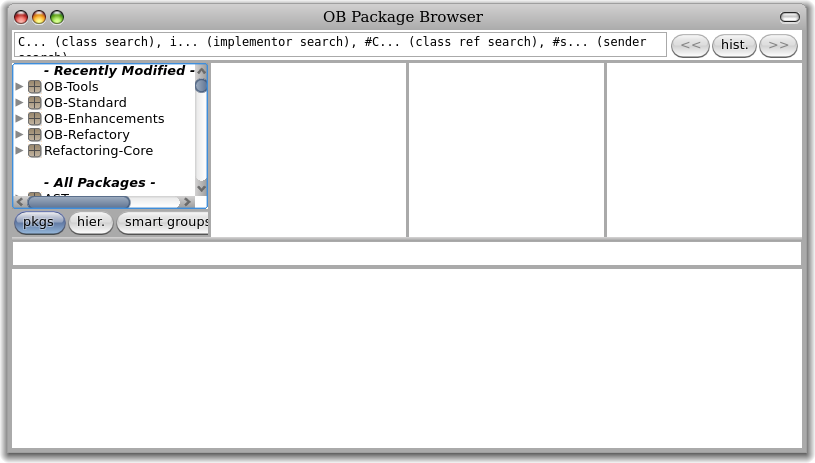
\includegraphics[width=0.7\textwidth]{SystemBrowser0} }
   \caption{El Navegador}
   \figlabel{SystemBrowser0}
\end{figure}

Los cuatro paneles pequeños en la parte superior del navegador representan una visi\'on jer\'arquica de los m\'etodos que se hallan en el sistema, de una manera muy similar a como el \textit{File Viewer} de \ind{NeXTstep} y el \textit{Finder} de Mac OS X en modo de columna, dan una vista de los archivos en el disco.
En el panel que se halla en el extremo ixquierdo se encuentran las listas de los \emph{paquetes} de clases; seleccione uno (por ejemplo \scat{Kernel}) y el panel a la derecha mostrar\'a entonces todas las clases en ese paquete.
% \on{I adopted the spelling of NeXTstep recommended by wikipedia}

\begin{figure}[htbp]
   \centering
   \ifluluelse
	   {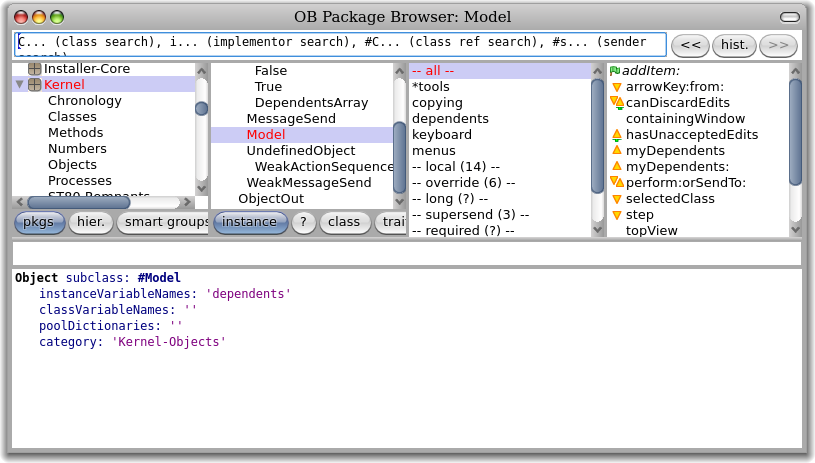
\includegraphics[width=\textwidth]{SystemBrowser1} }
	   {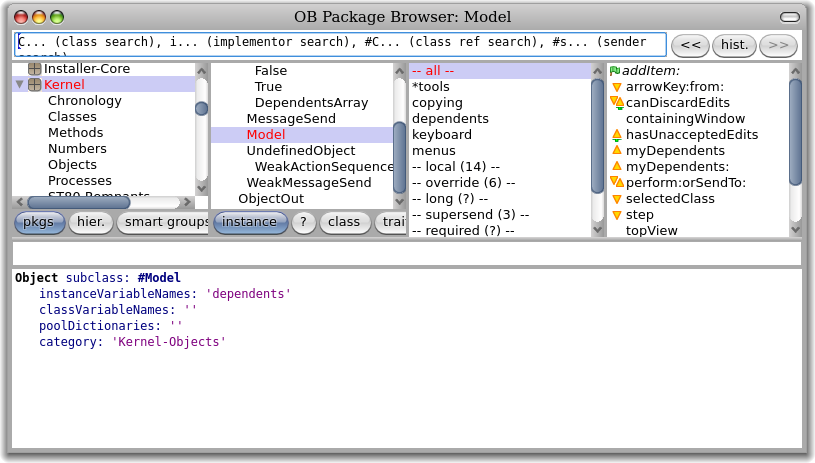
\includegraphics[width=.7\textwidth]{SystemBrowser1} }
   \caption{El Navegador con la clase \ct{Model} seleccionada
   \figlabel{SystemBrowserModel}}
\end{figure}

De forma similar, si selecciona una de las clases en el segundo panel, por ejemplo, \menu{Model} (v\'ease \figref{SystemBrowserModel}), el tercer panel mostrar\'a todos los \emph{protocolos} definidos para esa clase, asi como un protocolo virtual \prot{-{}-all-{}-}, que est\'a seleccionado por defecto.
Los protocolos son una forma de categorizar los m\'etodos; hacen m\'as facil hallar y pensar en en el comportamiento de una clase al separarla en piezas m\'as pequeñas y conceptualmente coherentes.
El cuarto panel muestra los nombres de todos los m\'etodos definidos en el protocolo seleccionado.
Si selecciona el nombre de un m\'etodo, el c\'odigo fuente del m\'etodo correspondiente aparece en el panel alergado en la parte inferior del navegador, donde puede verlo, editarlo, y guardar la versi\'on editada.
Si selecciona la clase \menu{Model}, el protocolo \protind{dependents} y el m\'etodo \menu{myDependents}, el navegador deber\'ia verse como en \figref{SystemBrowserMyDependents}.
\protindex{all}
\cmindex{Model}{myDependents}

\begin{figure}[htbp]
   \centering
   \ifluluelse
	   {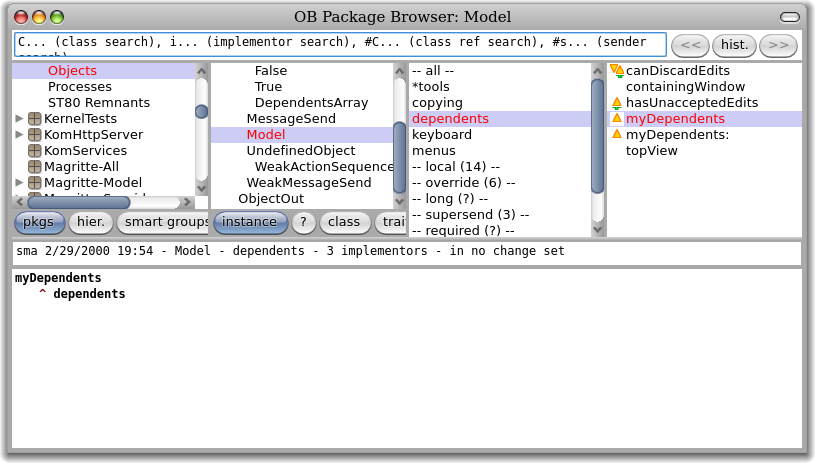
\includegraphics[width=\textwidth]{SystemBrowserMyDependents}}
	   {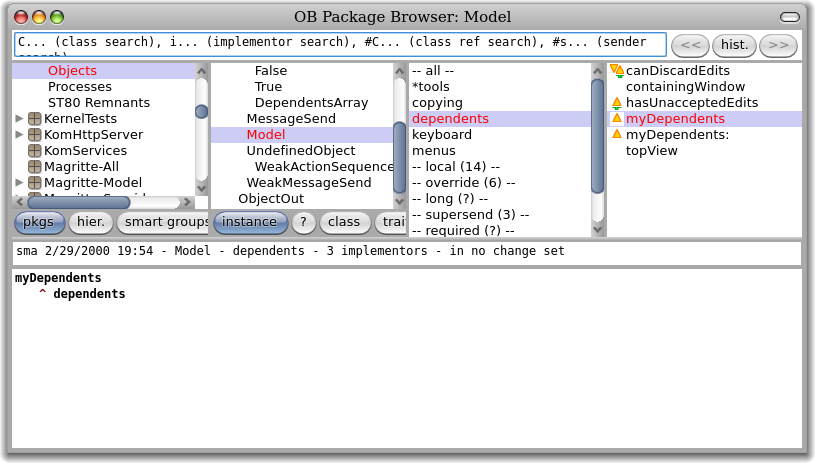
\includegraphics[width=0.7\textwidth]{SystemBrowserMyDependents}}
   \caption{El Navegador mostrando el m\'etodo \ct{myDependents} en la clase \ct{Model}
   \figlabel{SystemBrowserMyDependents}}
\end{figure}

A diferencia de los directorios en el \emph{Finder} de Mac OS X, los cuatro paneles superiores no son exactamente iguales.
Mientras que las clases y los m\'etodos son parte del lenguaje Smalltalk, los paquetes y protocolos no lo son: son una comodidad agregada por el navegador para limitar la cantidad de informaci\'on que debe ser mostrada en cada panel. Por ejemplo, si no hubiera protocolos, el navegador tendr\'ia que mostrar una lista de todos los m\'etodos en la clase seleccionada; para muchas clases esta lista ser\'ia muy extensa para ser recorrida convenientemente.
\index{Mac OS X Finder}

Por esta raz\'on, la manera de crear un nuevo paquete o protocolo es diferente de la forma en que se crea una nueva clase o m\'etodo. Para crear un nuevo paquete, haga click en el panel de paquetes y seleccione \menu{new package}; para crear un nuevo protocolo, haga click en el panel de protocolos y seleccione \menu{new protocol}.
Ingrese el nombre de este en el cuadro de dialogo, y est\'a listo: no hay nada m\'as en un paquete o protocolo que su nombre y su contenido.
\index{package!creating}

\begin{figure}[htbp]
   \centering
   \ifluluelse
	   {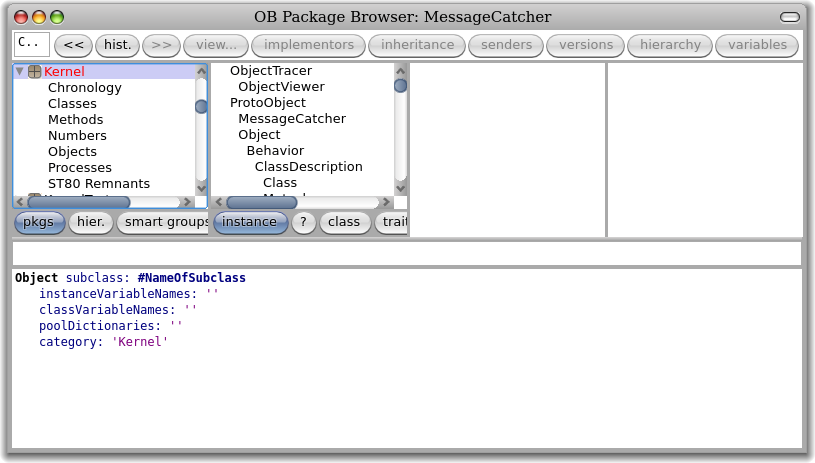
\includegraphics[width=\textwidth]{SystemBrowserClassCreation}}
	   {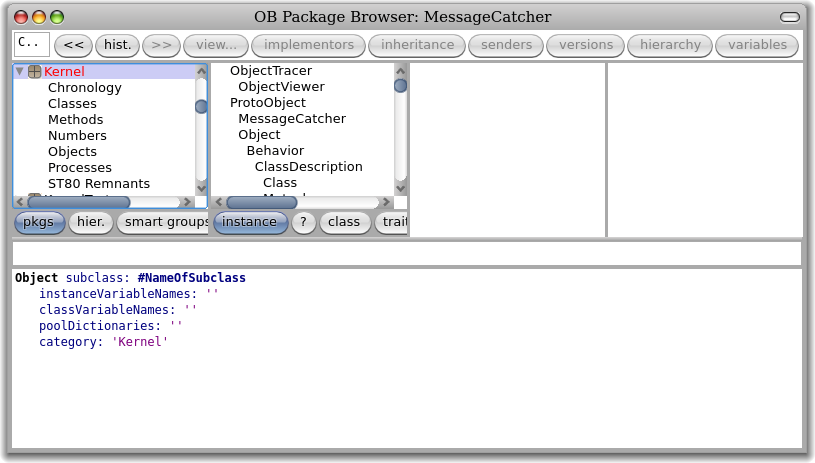
\includegraphics[width=0.7\textwidth]{SystemBrowserClassCreation}}
   \caption{El Navegador mostrando la plantilla de creaci\'on de clases
   \figlabel{SystemBrowserClassCreation}}
\end{figure}

Por otro lado, para crear una nueva clase o un nuevo m\'etodo, se deber\'a escribir
cierto c\'odigo Smalltalk. Si hace \click en el paquete
seleccionado(en el panel extremo izquierdo), el panel
inferior del navegador mostrar\'a la plantilla para la creaci\'on de la clase.
(\figref{SystemBrowserClassCreation}).  Se crea una nueva clase al
editar esta plantilla: reemplace \ct{Object} por el nombre de la clase existente
de la cual quiere crear una nueva subclase, reemplace
\ct{NameOfSubclass} por el nombre que desea darle a la nueva
subclase, y complete los nombres de las variables de instancia si los
conoce.  La categor\'ia de la nueva clase es por defecto la del paquete
que est\'e seleccionado\footnote{Recuerde que los paquetes y categor\'ias no son exactamente lo mismo. Se ver\'a la relaci\'on precisa en \secref{packages}}, pero puede cambiar esto tambi\'n si as\'i lo desea.  Si
ya tiene el navegador centrado en la clase de la que desea una
subclase, puede obtener la misma plantilla con unas pequeñas diferencias en la
inicializaci\'on mediante \actclick{ing} en el panel de clase, y
seleccionando \menu{class templates \ldots \go subclass template}.  Tambi\'en puede solo
editar la definici\'on de una clase existente, cambiando el nombre de la clase a
uno nuevo.  En todas las clases, cuando acepta la nueva definici\'on, la
nueva clase (aquella cuyo nombre est\'a a continuacion de \ct{#}) es creada (as\'i como
su correspondiente metaclase).  Crear una clase tambi\'en crea una variable global
que referencia a la clase, que es por lo que uno puede referirse a todas las
clases existentes por medio de usar sus nombres.  \index{class!creation}
\index{browser!defining a class}

Puede ver por qu\'e el nombre de la nueva clase tiene que aparecer como un \clsind{Symbol} (\ie antecedido por \ct{#}) en la plantilla de creaci\'on de la clase, pero despu\'es de que la clase ha sido creada, el c\'odigo puede referirse a la clase mediante usar el nombre como identificador (\ie sin el \ct{#})?

El proceso de creaci\'on de un nuevo m\'etodo es similar. Primero selecciona la clase en la que se desea que exista el m\'etodo, y luego se elige un protocolo.  El navegador mostrar\'a una plantilla de creaci\'on de m\'etodos, como se ve en \figref{SystemBrowserMethodTemplate}, la cual puede completar o editar.
\index{method!creation}
\index{browser!defining a method}

\begin{figure}[htbp]
   \centering
   \ifluluelse
	   {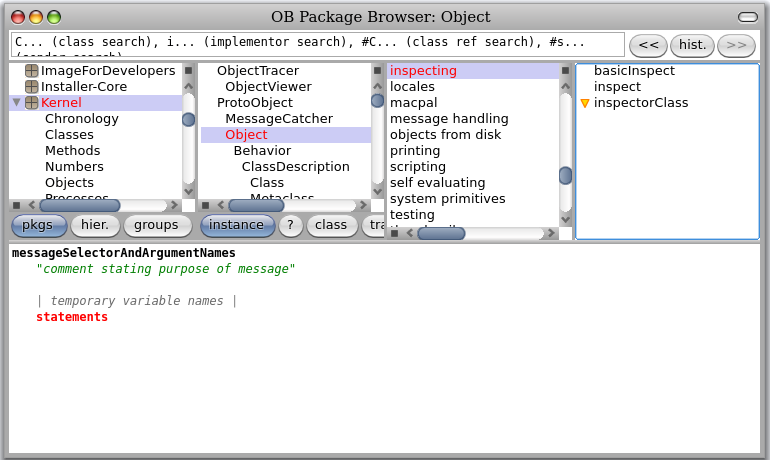
\includegraphics [width=\textwidth]{SystemBrowserMethodTemplate}}
	   {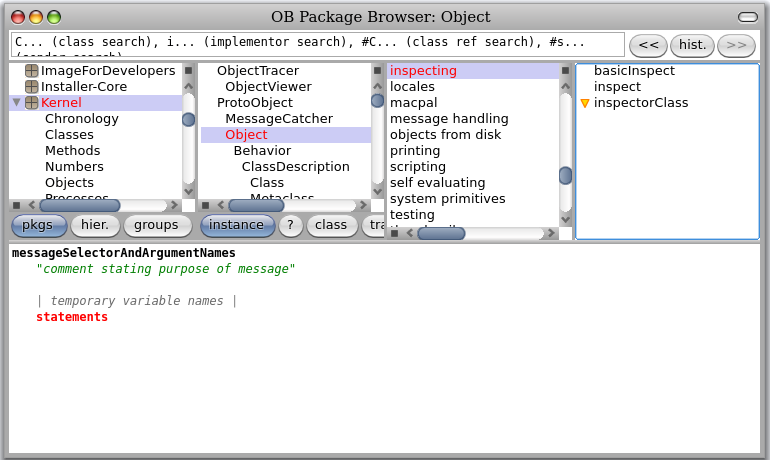
\includegraphics[width=0.7\textwidth]{SystemBrowserMethodTemplate}}
   \caption{El navegador mostrando la plantilla de creaci\'on de m\'etodos
   \figlabel{SystemBrowserMethodTemplate}}
\end{figure}

%---------------------------------------------------------
\subsection{Navegando los espacios de código}

El navegador provee varias herramientas para explorar y analizar código.
Estas herramientas pueden ser accedidas \actclick{ing} en varios de los menúes contextuales, o en el caso de las herramientas más frecuentemente usadas, por medio de un shortcut de teclado.\nicopaez{hace falta traducir shorcut??}

\subsubsection{Abriendo un nueva ventana del navegador}
\seclabel{browsing}

El ocasiones, querrás abrir múltiples ventanas de explorador.
Cuando estás escribiendo código seguramente necesitarás al menos dos: una para el método que estás escribiendo, y otra para navegar por el sistema para ver como funcionan las cosas.
You can open a browser on a class named by any selected text using the \short{b} \ind{keyboard shortcut}.
\index{browser!browse button}
\index{keyboard shortcut!browse it}

\dothis{Prueba esto: en un workspace, tipea el nombre de una clase (por ejemplo \ct{Morph}), seleccionalo, y presiona \short{b}. Este truco es frecuentemente útil; funciona en cualquier ventana de texto.}

\subsubsection{Emisores e implementadores de un mensaje}
\seclabel{sendersImplementors}

\index{browser!senders}
\Actclick{ing} \menu{browse \ldots \go senders (n)} en el panel de m\'etodos traer\'a una lista de todos los m\'etodos que puede usar el seleccionado m\'etodo. Con el navegador abierto en \ct{Morph}, haga clic en el m\'etodo \mthind{Morph}{drawOn:} en el panel de m\'etodos; el cuerpo de \ct{drawOn:} se mostrar\'a en la parte inferior del navegador. Si ahora seleccionas \menu{senders (n)} (\figref{SendersOfDrawOn}), aparecer\'a un men\'u con \ct{drawOn:} como el \'item mas alto, y abajo de este, todos los mensajes que \ct{drawOn:} env\'ia (\figref{SendersOfDrawOn2}).  Seleccionando un \'item en este men\'u abrir\'a el navegador con una lista de todos los m\'etodos en la imagen que env\'ia el seleccionado mensaje (\figref{CanvasDraw}).

%\begin{figure}[htb]
%\begin{minipage}[b]{0.74\textwidth}
%\centerline {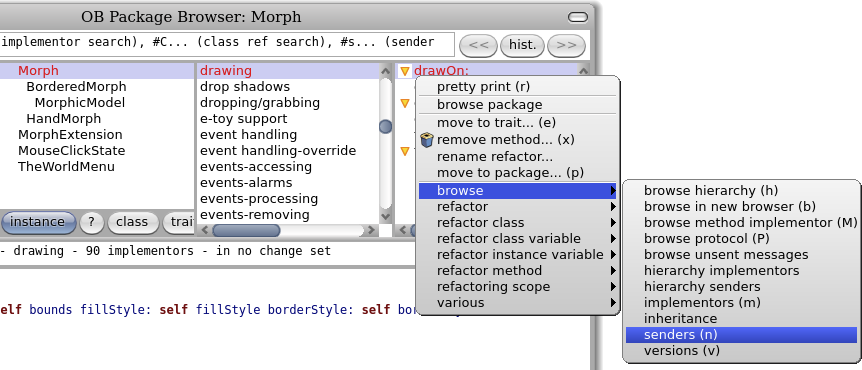
\includegraphics[width=\textwidth]{SendersOfDrawOn}}
%\caption{The \menu{senders (n)} menu item.\figlabel{SendersOfDrawOn}}
%\end{minipage}
%\hfill
%\begin{minipage}[b]{0.24\textwidth}
%\centerline {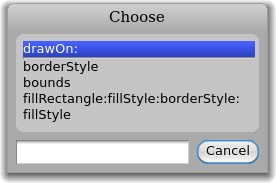
\includegraphics[width=\textwidth]{SendersOfDrawOn2}}
%\caption{Choose senders of which message.\figlabel{SendersOfDrawOn2}}
%\end{minipage}
%\end{figure}

\begin{figure}[htb]
\centerline {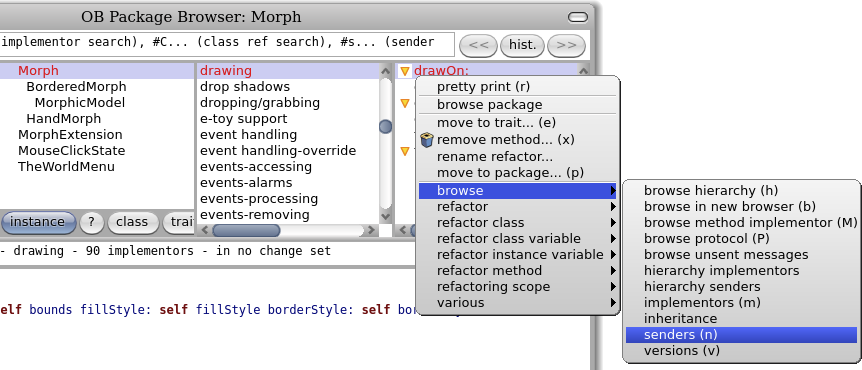
\includegraphics[width=\textwidth]{SendersOfDrawOn}}
\caption{The \menu{senders (n)} menu item.\figlabel{SendersOfDrawOn}}
\end{figure}

\begin{figure}[htb]
\centerline {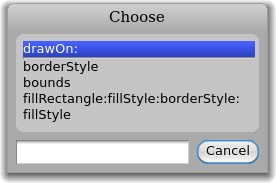
\includegraphics[width=0.4\textwidth]{SendersOfDrawOn2}}
\caption{Choose senders of which message.\figlabel{SendersOfDrawOn2}}
\end{figure}

La ``n'' en \menu{senders (n)} te indica que el acceso r\'apido del teclado para encontrar los emisores de un mensaje es \short{n}. Esto trabajar\'a en \emph{cualquier} ventana de texto.

\dothis{Seleccionar el texto ``drawOn:'' en el panel de c\'odigo y presionar \short{n} para inmediatamente traer los emisores de \ct{drawOn:}.}

\begin{figure}[htbp]
	\begin{center}
   \ifluluelse
		{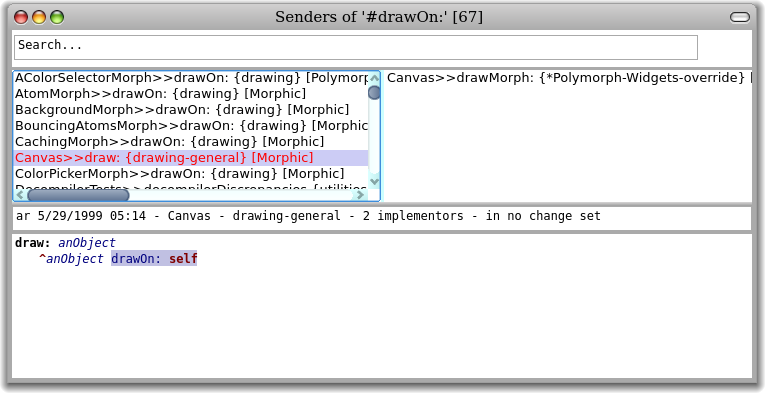
\includegraphics[width=\textwidth]{CanvasDraw}}
		{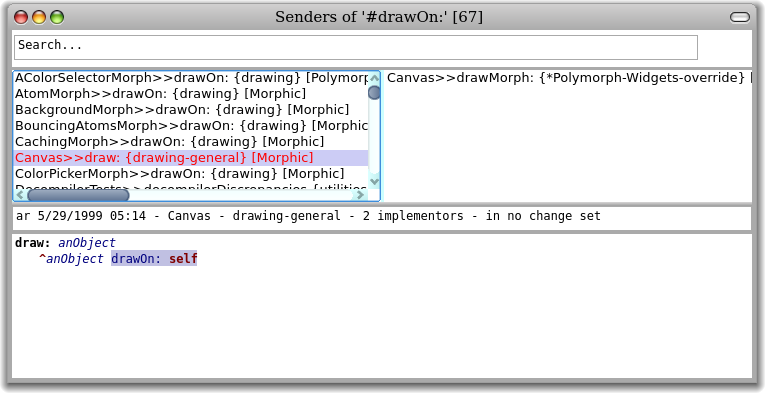
\includegraphics[width=0.7\textwidth]{CanvasDraw}}
	\end{center}
	\caption{The Senders Browser showing that the \ct{Canvas>>>draw} method sends the \ct{drawOn:} message to its argument.	\figlabel{CanvasDraw}}
\end{figure}

Si est\'as buscando los emisores de \ct{drawOn:} en \ct{AtomMorph>>>drawOn:}, ver\'as que esto es un super \subind{super}{send}.  Por lo tanto sabemos que el m\'etodo que se ejecutar\'a ser\'a en la superclase de \ct{AtomMorph} . Que clase es esta?  \Actclick ~ \menu{browse \go hierarchy implementors} y ver\'as que esta es \ct{EllipseMorph}.
\index{browser!hierarchy button}

Ahora mire el sexto emisor en la lista, \ct{Canvas>>>draw}, mostrado en la \figref{CanvasDraw}.
Usted puede ver que este m\'etodo env\'ia \ct{drawOn:}para cualquier objeto que se le pasa como un argumento, lo que potencialmente podr\'ia ser una instancia de cualquier clase.
An\'alisis de flujo puede ayudar a entender la clase del receptor de algunos mensajes, pero en general, no existe una manera sencilla para que el navegador pueda saber cual mensaje-env\'ia puede causar que los m\'etodos ser\'an ejecutados.
Por esta raz\'on, los ``senders''en el navegador muestra exactamente lo que sugiere su nombre: todos los emisores de los mensajes con el selector elegido.
El navegador de emisores es sin embargo extremadamente \'util cuando necesitas comprender c\'omo puedes \emph{usar} un m\'etodo: te permite navegar r\'apidamente a trav\'es del ejemplo utilizado.
Dado que todos los m\'etodos con el mismo selector deben usarse de la misma manera, todos los usos de un determinado mensaje tienen que ser similares.
\index{browser!senders}

\index{browser!implementors}
El navegador de los implementadores trabaja de una manera similar, pero en vez del listado de emisores de un mensaje, esto lista todas las clases que implementan un m\'etodo con el mismo selector. Para ver esto, seleccione \lct{drawOn:} en el panel de m\'etodos y seleccione \menu{browse \go implementors (m)} (o seleccione el texto ``drawOn:'' en el panel de c\'odigo y presione \short{m}).
Deber\'ias obtener una ventana con una lista de m\'etodos mostrando una lista desplazable de 90-odd clases que implementa un m\'etodo \ct{drawOn:}.
No deber\'ia ser tan sorprendente que tantas clases implementen este m\'etodo: \ct{drawOn:} es el mensaje que se entiende por cada objeto que es capaz de representarse en la patalla.

\subsubsection{Versiones de un m\'etodo}
\seclabel{versions}

Cuando guardas un nuevo \subind{m\'etodo}{versi\'on} de un m\'etodo, la antigua no se pierde.  \pharo mantiene todas las versiones antiguas, y te permite comparar las diferentes versiones y volver (``revert'') a una versi\'on antigua.
\begin{figure}[btp]
   \centering
   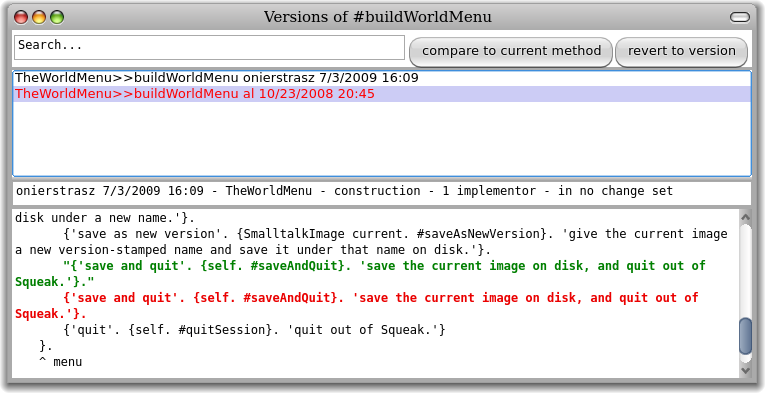
\includegraphics[width=\textwidth]{Versions}
   \caption{The \ind{versions browser} showing two versions of the \ct{TheWorldMenu>>>buildWorldMenu:} method}
   \figlabel{buildWorldMenuVersions}
\end{figure}
El \'item del men\'u \menu{browse \go versions (v)} da acceso a las sucesivas modificaciones introducidas en el m\'etodo seleccionado.
En \figref{buildWorldMenuVersions} podemos ver dos versiones del m\'etodo \ct{buildWorldMenu:}.

\index{browser!versions button}
El panel superior muestra una l\'inea para cada versi\'on del m\'etodo, en el que fifuran las iniciales del programador que las escribi\'o, la fecha y hora en que se guard\'o, los nombres de la clase y el m\'etodo, y el protocolo en el que se ha definido.  La actual versi\'on (activa) est\'a en la parte superior de la lista; independiente de la versi\'on seleccionada se muestra en la parte inferior del panel.
% Si el checkbox \menu{diffs} esta seleccionado, como lo es en \figref{mouseUpVersions}, la pantalla tambi\'en muestra las diferencias entre la versi\'on seleccionada y el inmediatamente anterior.
Tambi\'en se proporcionan botones para mostrar las diferencias entre el m\'etodo seleccionado y la versi\'on actual, y para volver a la versi\'on seleccionada.
% El checkbox \menu{prettyDiffs} es \'util si ha habido cambios en el dise�o: este imprime muy bonito ambas versiones antes de la diferenciaci\'on, de modo que las diferencias que se observan excluyen los cambios del formato.

La existencia de las \ind{versiones del navegador} significa que nunca tend\'as que preocuparte de preservar el c\'odigo que piensas que tal ves ya no sea necesario: simplemente suprimalo. Si encuentr\'as que lo \emph{necesitas}, siempre puedes volver a la versi\'on anterior, o copiar el fragmento de la versi\'on anterior y pegarlo en otro m\'etodo.
Get into the habit of using versions;  ``comentando'' el c\'odigo que ya no es necesario es una mala pr\'actica porque hace que el actual c\'odigo sea m\'as dif\'icil de leer.
La tasa de legilibilidad de c\'odigo de Smalltalkers es extremadamente alta.

\hint{Que pasa si se elimina completamente un m\'etodo?, y luego se decides que deseas recuperarlo?  Puedes encontrar el borrado en un conjunto de cambio, donde puedes pedir ver las versiones por \actclick{ing}.
El conjunto de cambio est\'a descrito en \secref{env:changeSet}}

\subsubsection{Sobre escribiendo m\'etodos}
\seclabel{overriding}

El navegador de herencia mostrar\'a todos los m\'etodos sobre escritos por el m\'etodo mostrado.
Para ver como trabaja, seleccione el m\'etodo \cmind{ImageMorph}{drawOn:} en el navegador.
Nota el icono triangular pr\'oximo al nombre del m\'etodo (\figref{OBinheritanceBrowser}).
El tri\'angulo que apunta hacia arriba te dice que \ct{ImageMorph>>>drawOn:} sobre escribe un m\'etodo heredado (\ie \ct{Morph>>>drawOn:}), y el tri\'angulo apuntando hacia abajo te dice que es sobre escrito por subclases. (Tambi\'en puedes hacer click sobre los iconos para ir a estos m\'etodos.)
Ahora selecciona \menu{browse \go inheritance}.
El navegador de herencia te mostrar\'a la jerarqu\'ia de los m\'etodos sobre escritos (ver \figref{OBinheritanceBrowser}).

\begin{figure}[btp]
	\begin{center}
   \ifluluelse
		{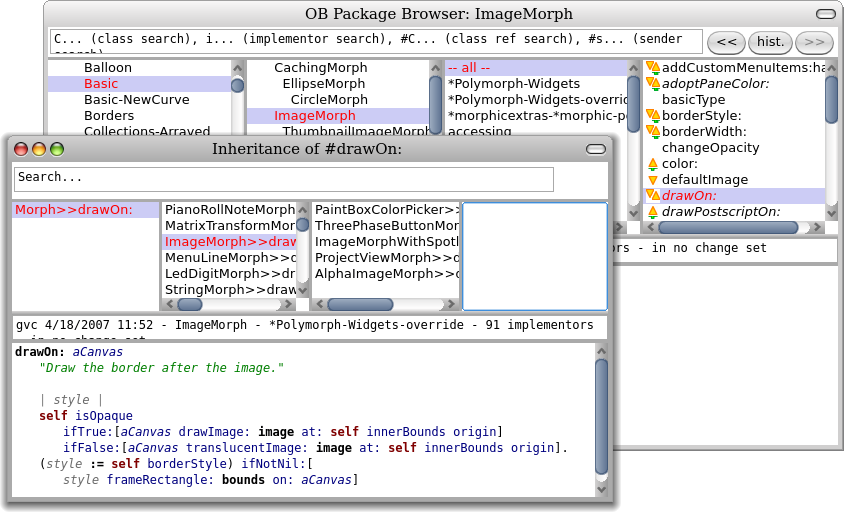
\includegraphics[width=\textwidth]{OBInheritanceOverriding}}
		{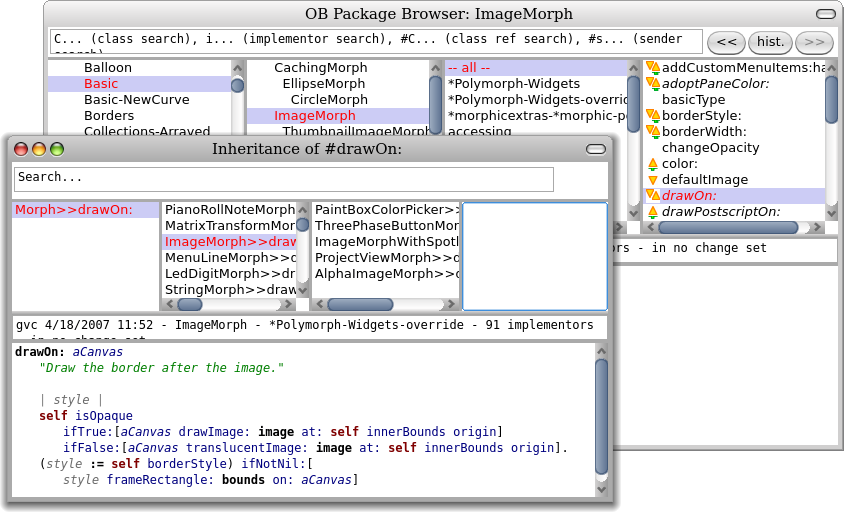
\includegraphics[width=0.7\textwidth]{OBInheritanceOverriding}}
	\end{center}
	\caption{\ct{ImageMorph>>>drawOn:} y los m\'etodos que este sobre escribe. Los hermanos de los m\'etodos seleccionados son mostrados en las listas de desplazables.}
	\figlabel{OBinheritanceBrowser}
\end{figure}

\subsubsection{La vista de jerarqu\'ia}
\seclabel{hierarchy}

De forma predeterminada, el navegador presenta una lista de los paquetes en el panel que est\'a m\'as a la izquierda.
Sin embargo, es posible cambiar a una vista de jerarqu\'ia de clases.
Simplemente seleccione una clase de particular de inter\'es, tal como  \ct{ImageMorph} y, haga clic en el bot\'on \button{hier.}.
A continuaci\'on, podr\'a ver en el panel que est\'a m\'as a la izquierda una jerarqu\'ia de clases mostrando todas las superclases y subclases de la clase seleccionada.
El segundo panel muestra los paquetes que implementan los m\'etodos de la clase seleccionada.
%El bot\'on \button{hierarchy} abre un \ind{navegador de jerarqu\'ia} en la actual clase; este
%navegador puede tambi\'en ser abierto utilizando el \'item del men\'u \menu{browse hierarchy} en el panel de clases.
%El navegador de la jerarqu\'ia es similar al navegador, pero en vez de mostrar las categor\'ias y las clases en cada categor\'ia, muestra una \'unica lista de clases, indentada para representar la jerarqu\'ia.
%La categor\'ia de la seleccionada clase es mostrada en un peque�o panel de comentarios en la parte superior del navegador.
El navegador de jerarqu\'ia \figref{hierarchyBrowser}, revela que la superclase directa de \clsind{ImageMorph} es \clsind{Morph}.
\index{browser!hierarchy button}

\begin{figure}[btp]
	\begin{center}
	\ifluluelse
		{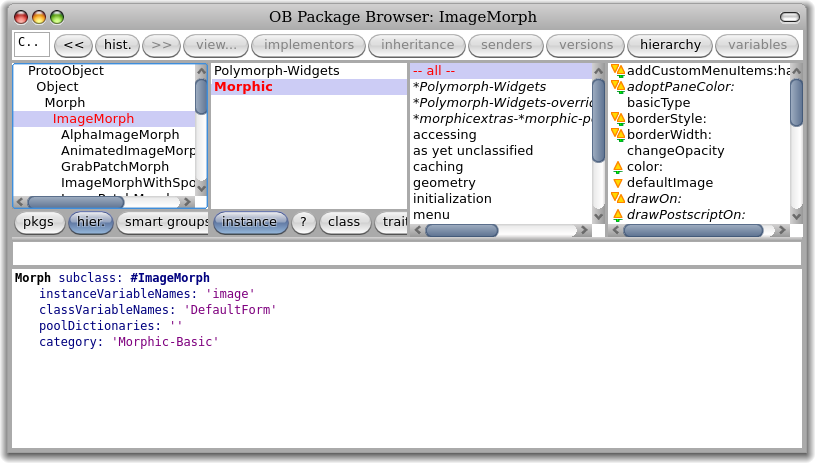
\includegraphics[width=\textwidth]{hierarchyBrowser}}
		{\includegraphics[width=0.7\textwidth]{hierarchyBrowser}}
	\end{center}
	\caption{A hierarchy view of \ct{ImageMorph}.}
	\figlabel{hierarchyBrowser}
\end{figure}

\subsubsection{Encontrar las referencias a variables}
\seclabel{variables}

\index{browser!variables}
Por\actclick{ing} en una clase en el panel de clases, y seleccionando \menu{browse \go chase variables}, puedes encontrar donde se utiliza una variable de clase o una variable de instancia.
Se le presentar\'a con un \emph{chasing browser} que le permitir\'a recorrer los descriptores de acceso de todas las variables de instancia y las variables de clases , y, a su vez, los m\'etodos que envian estos descriptores, etc. (\figref{chasingBrowser}).

\begin{figure}[btp]
	\begin{center}
	\ifluluelse
		{\includegraphics[width=\textwidth]{chasingBrowser}}
		{\includegraphics[width=0.7\textwidth]{chasingBrowser}}
	\end{center}
	\caption{Un navegador de seguimiento para \ct{Morph}.}
	\figlabel{chasingBrowser}
\end{figure}

% The menu also includes \menu{inst var defs}, which shows the subset of the instance variable references that assign to the variable.
%Once you click on the button or select the menu item, you will be presented with a dialog that invites you to choose a variable from all of the variables defined in the current class, and all of the variables that it inherits.  The list is in inheritance order; it can often be useful to bring up this list just to remind yourself of the name of an instance variable.  If you click outside the list, it will go away and no variable browser will be created.

%Also available by \actclick{ing} the class pane is \menu{class vars}, which opens an inspector showing the class variables of the current class \emph{and their values}, and \menu{class refs (N)} which displays a list of all of the methods that directly reference the current class.

\subsubsection{Fuente}
\seclabel{sources}

\index{browser!view}
El item del men\'u \menu{various \go view \ldots} disponible por \actclick{ing} en el panel del m\'etodo trae el men\'u ``how to show'', el cual te permite escoger como el navegador mostrar\'a el m\'etodo seleccionado en el panel de fuente. Las opciones incluyen el c\'odigo \menu{fuente}, el c\'odigo fuente \menu{prettyPrint}ed , \menu{byteCode} y el c\'odigo fuente \menu{decompile}d desde los c\'odigos byte.
% The label on the button changes if you select one of the other modes.  There are other options too; if you let the mouse linger over the names, a help balloon will appear.  Try some of them.
\index{method!pretty-print}
\index{method!decompile}
\index{method!byte code}

Tenga en cuenta que seleccionando \menu{prettyPrint} en el men\'u ``how to show'' \emph{no} es lo mismo como el resaltado de sintaxis de un m\'etodo antes de guardarlo \footnote{\menu{pretty print (r)} es el primer \'item en el panel de m\'etodo, o en la mitad hacia abajo en el panel de c\'odigo.}.
Los controles del men\'u solamente como muestra el navegador, y no tiene efecto sobre el c\'odigo almacenado en el sistema.
Esto lo puedes comprobar abriendo dos navegadores, y seleccionando en uno \menu{prettyPrint} y en el otro \menu{source}.
De hecho, focalizando dos navegadores en el mismo m\'etodo y seleccionando en uno \menu{byteCode} y en el otro \menu{decompile} es una buena forma de aprender acerca del conjunto de instrucciones byte-coded de la m\'aquina virtual \pharo.

\subsubsection{Refactorizaci\'on}

Los men\'ues contextuales ofrecen un gran n\'umero de refactorizaciones est\'andares.
Simplemente \actclick en cualquiera de los cuatro paneles para ver las operaciones de refactorizaci\'on actualmente disponibles.
Ver \figref{refactoring}.

La Refactorizaci\'on estubo previamente disponible solamente en un navegador especial llamado navegador de refactorizaci\'on, pero ahora se puede acceder a este desde cualquier navegador.

\begin{figure}[btp]
	\begin{center}
	\ifluluelse
		{\includegraphics[width=\textwidth]{refactoring}}
		{\includegraphics[width=0.7\textwidth]{refactoring}}
	\end{center}
	\caption{Operaciones de Refactorizaci\'on.}
	\figlabel{refactoring}
\end{figure}

%---------------------------------------------------------
\subsection{Los men\'us de navegaci\'on}

Muchas funciones adicionales est\'an disponibles por \actclick{ing} en los paneles del navegador.
Incluso si las etiquetas sobre los \'items del men\'u son los mismos, su \emph{significado} puede ser dependiente del contexto.
Por ejemplo, el panel de paquetes, el panel de clases, el panel de protocolos y el panel de m\'etodos todos tienen un \'item del men\'u \menu{file out}.  Sin embargo, ellas hacen cosas diferentes: del men\'u del panel de paquetes \menu{file out} emerge el paquete completo, del men\'u del panel de clases \menu{file out} emerge la clase completa, del men\'u del panel de protocolos \menu{file out} emerge el protocolo completo, y del men\'u del panel de m\'etodos \menu{file out} emerge solo el m\'etodo mostrado.
Si bien esto puede parecer obvio, puede ser una fuente de confusi\'on para los principiantes.
\index{file!filing in}
\index{file!filing out}

Posiblemente el \'item del men\'u mas \'util es \menu{find class\ldots (f)} en el panel de packetes.  Aunque las categor\'ias son \'utiles para el c\'odigo que estamos desarrollando activamente, la mayor\'ia de nosotros no sabemos la categorizaci\'on de todo el sistema, y es mucho mas r\'apido escribir \short{f} seguido por los primeros caracteres del nombre la clase que adivinar cual paquete podr\'ia estar adentro.  \menu{recent classes\ldots} tambi\'en puede ayudarte a volver r\'apidamente a una clase por la cual se ha navegado recientemente, incluso si haz olvidado su nombre.
\index{class!finding}
\index{class!recent}

Tambi\'en puedes buscar una clase o m\'etodo espec\'ifico tecleando el nombre en el recuadro de b\'usqueda en el cuadro superior izquierdo del navegador. Cuando presiones return, una consulta ser\'a puesta en el sistema, y los resultados de la consulta ser\'an mostrados.  Tenga en cuenta que anteponiendo su con sulta con \ct{#}, puedes buscar las referencias a una clase o emisores de un mensaje.
%To browse to a particular method, you can
%In the class pane, there are two menu items \menu{find method} and \menu{find method wildcard\ldots} that can be useful if you want to browse a particular method.
Si est\'as buscando un m\'etodo en particular de la clase seleccionada, es a menudo mas r\'apido it is often quicker to browse the \prot{-{}-all-{}-} protocol (que es el valor predeterminado), coloque el mouse en el panel del m\'etodo, y escriba la primera letra del nombre del m\'etodo que est\'as buscando.
Esto usualmente desplazar\'a el panel de modo que la b\'usqueda del nombre del m\'etodo sea visible.
\index{method!finding}
\protindex{all}

\dothis{Trate de navegar en ambas formas para \cmind{OrderedCollection}{removeAt:}}

Hay muchas otras opciones disponibles en los men\'ues. Por eso es mejor pasar unos minutos trabajando con el navegador y ver lo que hay.

\dothis{Compare el resultado de \menu{Browse Protocol}, \menu{Browse Hierarchy}, y \menu{Show Hierarchy} en el men\'u del panel de clases.}

%---------------------------------------------------------
\subsection{Navegar mediante programaci\'on}

La clase \glbind{SystemNavigation} proporciona una serie de m\'etodos de utilidad que son \'utiles para navegar por el sistema.
Muchas de las funciones ofrecidas por el cl\'asico navegador son implementadas por \ct{SystemNavigation}.
\index{browsing programmatically}

\dothis{
Abrir un espacio de trabajo y evaluar el siguiente c\'odigo para navegar por los emisores de \ct{drawOn:}:}
\begin{code}{}
SystemNavigation default browseAllCallsOn: #drawOn:
\end{code}
Para restringir la b\'usqueda de los remitentes a los m\'etodos de una clase espec\'ifica:
\begin{code}{}
SystemNavigation default browseAllCallsOn: #drawOn: from: ImageMorph
\end{code}
Debido a que las herramientas de desarrollo son objetos, que son completamente accesibles desde programas, puedes desarrollar tus propias herramientas o adaptar las herramientas existentes para tus necesidades.

El equivalente en programaci\'on al nem\'u \menu{implementors} es:
\begin{code}{}
SystemNavigation default browseAllImplementorsOf: #drawOn:
\end{code}

Para conocer m\'as acerca de lo que est\'a disponible, explorar la clase \ct{SystemNavigation} con el navegador.
Adicionales ejemplos de navegaci\'on pueden ser encontrados en las preguntas frecuentes FAQ (\appref{faq}).

%=========================================================
\section{Monticello}

Hemos dado un r\'apido repaso de \ind{Monticello}, el paquete de herramientas de \pharo, en \secref{Monticello}.
Sin embargo, Monticello tiene muchas mas caracter\'isticas que se han discutido.
Debido a que Monticello administra \emph{paquetes}, Antes de hablarles m\'as acerca de Monticello, es importante que expliquemos primero exactamente lo que es un \ind{paquete} .

%---------------------------------------------------------
\subsection{Packages: declarative categorization of \pharo code}\seclabel{packages}

Hemos indicado anteriormente, en \secref{categoriesPackages} los paquetes que son m\'as o menos equivalentes a las categor\'ias. Ahora vamos a ver exactamente cu\'al es la relaci\'on.
El sistema de paquetes es un sencilla y simple manera de organizar el c\'odigo fuente smalltalk que explota una simple convenci\'on de nombres para las categor\'ias y protocolos.

Veamos esto utilizando un ejemplo.
Suponga que est\'a desarrollando un framework determinado con el fin de facilitar la utilizaci\'on de bases de datos relacionales de \pharo. Han decidido llamar al framework \ct{PharoLink}, y han creado una serie de categor\'ias que contienen todas las clases que se han escrito, ejemplo de categor\'ia \ct{'PharoLink-Connections'} contiene \ct{OracleConnection MySQLConnection PostgresConnection} y la categor\'ia \ct{'PharoLink-Model'} contiene \ct{DBTable DBRow DBQuery}, etc. Sin embargo, no todo el c\'odigo residir\'a en estas clases. Por ejemplo, tambi\'en puede tener una serie de m\'etodos para convertir objetos en un formato amistoso de SQL:

\begin{code}{}
Object>>>asSQL
String>>>asSQL
Date>>>asSQL
\end{code}

\noindent
Estos paquetes pertenecen a
% \damien{don't we say 'belong to'?}
% \on{no -- belong in = they should be there; belong to = they are there}
los mismos paquetes como las clases en las
categor\'ias \ct{PharoLink-Connections} y \ct{PharoLink-Model}.
Pero es evidente que el conjunto completo de la clase \ct{Object} no pertenece a tu paquete!
Por lo tanto necesitas una manera de poner ciertos \emph{m\'etodos} en un paquete, aunque el resto de la clase est\'a en otro paquete.
\index{package!extension}
\seeindex{extension package}{package, extension}

La manera en que lo haces es poniendo esos m\'etodos en un protocolo  (of \ct{Object}, \ct{String}, \ct{Date}, y as\'i sucesivamente) llamado \prot{*PharoLink} (nota el primer asterisco). La combinaci\'on de las categor\'ias \scat{PharoLink-\ldots} y los protocolos \prot{*PharoLink} forman un paquete denominado \ct{PharoLink}.
Para ser m\'as precisos, las normas de lo que va en un paquete son de la siguiente manera.

Un paquete llamado \ct{Foo} contiene:

\begin{enumerate}		\seclabel{packageRules}
	\item{} todas las \emph{definiciones de la clase} de las clases en la categor\'ia \scat{Foo}, o en las categor\'ias que comienzan con \scat{Foo-}, y
	\item{} \label{env:extensions} todos los \emph{m\'etodos} en \emph{cualquier clase} en los protocolos llamados \prot{*Foo} o \prot{*foo}\footnote{Al realizar esta comparaci\'on, las letras may\'usculas y min\'usculas  en los nombres son ignoradas.}, o cuyo nombre comience con \prot{*Foo-} or \prot{*foo-}, y
	\item{} todos los \emph{m\'etodos} en las clases de la categor\'ia \scat{Foo}, o en la categor\'ia cuyo nombre comience con \scat{Foo-}, \emph{excepto} para esos nombres en los protocolos cuyos nombres comienzan con \prot{*}.
	
\end{enumerate}
\noindent
Una consecuencia de estas reglas es que cada definici\'on de clase y cada m\'etodo pertenece a exactamente un paquete. La \emph{excepci\'on} en la \'ultima regla ha de estar all\'i porque esos m\'etodos deben pertenecer a otros paquetes. La raz\'on para ignorar el  case en la regla \ref{env:extensions} es que, por convenci\'on, los nombres de los protocolos son normalmente (pero no necesariamente) nim\'usculas (y puede incluir espacios), mientras los nombres de las categor\'ias usan CamelCase (y no incluyen espacios).
\index{camelCase}

La clase \ct{PackageInfo} implementa estas reglas, y una manera de tener una sensaci\'on de ellos es experimentar con esta clase.

\dothis{Eval\'ue la siguiente expresi\'on en un workspace:}

\begin{code}{}
mc := PackageInfo named: 'Monticello'
\end{code}

Ahora es posible mirar al interior de este paquete.
Por ejemplo, imprimiendo \ct{mc classes} en el panel del workspace pane devolver\'a una larga lista de clases que componen el paquete de Monticello.
\ct{mc coreMethods}
devolver\'a una lista de \ct{MethodReference}s para todos los m\'etodos en esas clases. \ct{mc extensionMethods} es quiz\'as una de las m\'as interesantes consultas: esta devolver\'a una lista de todos los m\'etodos contenidos en el paquete \ct{Monticello} pero no contenido dentro de una clase \lct{Monticello}.

Los paquetes son una adici\'on relativamente nueva a \pharo, pero ya que las convenciones de nombres de paquetes se basaron en los que estaban en uso, es posible usar \ct{PackageInfo} para analizar c\'odigo m\'as antiguo que no ha sido expl\'icitamente adaptado para trabajar con \'el.

\dothis{Print \ct{(PackageInfo named: 'Collections') externalSubclasses}; esta expresi\'on responder\'a con una lista de todas las subclases de  \ct{Collection} que \emph{no} est\'an en el paquete \ct{Collections}. }

%---------------------------------------------------------
\subsection{Monticello b\'asicos}

\ind{Monticello} debe su nombre al hogar de Thomas Jefferson, una mansi\'on neocl\'asica constru\'iada en la cima de un cerro , tercer presidente de los Estados Unidos y autor del Estatuto de libertad Religiosa de Virginia. El nombre significa ``mont\'iculo'' en Italiano, y por lo tanto, se pronuncia siempre con una ``c'' italiana, que suena como el ``ch'' en chair: Mont-y'-che-llo.


\begin{figure}[btp]
	\begin{center}
	\ifluluelse
		{\includegraphics[width=\textwidth]{freshMonticello}}
		{\includegraphics[width=0.7\textwidth]{freshMonticello}}
	\end{center}
	\caption{El navegador de Monticello.}
	\figlabel{freshMonticello}
\end{figure}

Al abrir el navegador de Monticello, ver\'as dos paneles de lista y una fila de botones, como se muestra en \figref{freshMonticello}.
El panel de la izquierda muestra una lista de todos los paquetes que han sido cargados en la imagen que est\'as ejecutando; la versi\'on particular del paquete se muestra entre par\'entesis despu\'es del nombre.

El panel de la derecha muestra una lista de todos los repositorios de c\'odigo fuente que Monticello tiene conocimiento, usualmente porque se ha cargado el c\'odigo desde ellos.  Si seleccionas un paquete en el panel de la izquierda, el panel de la derecha se filtra para mostrar \'unicamente los repositorios que contienen las versiones del paquete seleccionado.

Uno de los repositorios es un directorio llamado \emph{package-cache}, el cual es un subdirectorio del directorio en el cual est\'as corriendo la imagen.
Cuando cargas el c\'odigo desde o escribes c\'odigo a un repositorio remoto, una copia es guardada en el cache del paquete. Esto puede ser \'util si la red no esta disponible y necesitas acceder a un paquete.  Tambi\'en, si le das un archivo Monticello (.mcz) directamente, por ejemplo como un archivo adjunto al correo electr\'onico, la forma m\'as conveniente de acceder a este es colocarlo en el directorio del package-cache.
\index{package!cache}

Para agregar un nuevo repositorio a la lista, clic en el \button{+Repository}, y elegir el tipo de repositorio en el men\'u emergente.  Vamos a agregar un repositorio HTTP.

\dothis{Open Monticello, click on \button{+Repository}, and select \menu{HTTP}.
Editar el di\'alogo para leer:}
%\ab{How does one continue the $\backslash$dothis to include the code?}
%\on{Don't.  Just close the \dothis{} and follow with the code.}
\needlines{4}
\begin{code}{}
MCHttpRepository
	location: 'http://squeaksource.com/PharoByExample'
	user: ''
	password: ''
\end{code}

\begin{figure}[btp]
	\begin{center}
	\ifluluelse
		{\includegraphics[width=0.7\textwidth]{SqueakSource-PBE}}
		{\includegraphics[width=0.7\textwidth]{SqueakSource-PBE}}
	\end{center}
	\caption{Un navegador de Repositorio.}
	\figlabel{SqueakSource:PBE}
\end{figure}
\noindent
Entonces cic en \button{Open} para abrir el navegador de repositorios en este directorio.  Dever\'ias ver algo como \figref{SqueakSource:PBE}.  A la izquierda hay una lista de todos los paquetes en el repositorio; si seleccionas uno, y luego el panel de la derecha se mostrar\'an todas las versiones del paquete seleccionado en este repositorio.

Si haz seleccionado una de las versiones, puedes usar el bot\'on \button{Browse} (sin cargarlo en tu imagen), bot\'on \button{Load} , o buscar con el bot\'on \button{Changes} que se har\'an a su imagen por la carga de la versi\'on seleccionada. Puedes tambi\'en hacer una \button{Copy} de la versi\'on del paquete, que luego puedes escribir en otro repositorio.

Como puedes ver, los nombres de las versiones contienen el nombre del paquete, las iniciales del autor de la versi\'on, y un n\'umero de versi\'on.  El nombre de la versi\'on es tambi\'en el nombre del archivo en el repositorio.  Nunca se deben cambiar estos nombres; la correcta operaci\'on de Monticello depende de ellos!   Los archivos de versiones Monticello son solo archivos zip, y si eres curioso puedes descomprimirlos con una herramienta zip, pero la mejor manera de mirar su contenido es usando el mismo Monticello.

Para crear un paquete con Monticello, tienes que hacer dos cosas: escribir alg\'un c\'odigo, y decile a Monticello acerca de esto.

\dothis{Crear un paquete llamado \scat{PBE-Monticello}, y poner un par de clases en este, como se muestra en \figref{MCnewcategory}.  Tambi\'en, crear un m\'etodo en una existente clase, tal como \ct{Object}, y ponerlo en el mismo paquete como sus clases, usando las reglas de la p\'agina \pageref{sec:packageRules}\,---\,ver \figref{MCnewmethod}.}

\begin{figure}[btp]
	\begin{center}
	\ifluluelse
		{\includegraphics[width=\textwidth]{MCnewcategory}}
		{\includegraphics[width=0.7\textwidth]{MCnewcategory}}
	\end{center}
	\caption{Dos clases en el paquete ``PBE''.}
	\figlabel{MCnewcategory}
\end{figure}

\begin{figure}[btp]
	\begin{center}
	\ifluluelse
		{\includegraphics[width=\textwidth]{MCnewmethod}}
		{\includegraphics[width=0.7\textwidth]{MCnewmethod}}
	\end{center}
	\caption{Una extensi\'on del m\'etodo que tambi\'en est\'a en el paquete ``PBE''.}
	\figlabel{MCnewmethod}
\end{figure}

Para decirle a Monticello acerca de tus paquetes, clic en el bot\'on \button{+Package}, y escriba el nombre del paquete, en este caso ``PBE''.  Monticello agregar\'a \ct{PBE} a su lista de paquetes; la entrada del paquete ser\'a marcada con un asterisco para mostrar que la versi\'on en la imagen todav\'ia no se ha escrito a cualquier repositorio. Tenga en cuenta que ahora deber\'as tener dos paquetes en Monticello, uno llamado \ct{PBE} y el otro llamado \ct{PBE-Monticello}. Esto esta bien, porque \ct{PBE} contendr\'a \ct{PBE-Monticello}, y otros paquetes a partir de \ct{PBE-}.

Inicialmente, el \'unico repositorio asociado con este paquete ser\'a su cache paquete, como se muestra en \figref{MC+PBE}.  Esto esta bien: todav\'ia puedes guardar el c\'odigo, lo que causar\'a que se escriba el la cach\'e del paquete.
Simplemente haz clic en el bot\'on \button{Save} y ser\'as invitado a proporcionar un registro de la versi\'on del paquete que est\'as a punto de guardar, como se muestra en \figref{PBE-on}; cuando aceptas el mensaje, Monticello guardar\'a tu paquete.
Para indicar esto, el asterisco decorando el nombre en el paquete en el panel de Monticello ser\'a eliminado, y se agregar\'a el n\'umero de la versi\'on.

Si a continuaci\'on haces un cambio en el paquete\,---\, por ejemplo agregando un m\'etodo a una de las clases\,---\, el asterisco volver\'a a aparecer, mostrando que tienes cambios que no han sido guardados.  Si abres un navegador de repositorio en el cach\'e de paquetes, puedes seleccionar la versi\'on guardada, y usar el bot\'on \button{Changes} y otros botones.
Tambi\'en puedes por su puesto guardar la nueva versi\'on al respositorio; una vez que refrescada con el bot\'on \button{Refresh} la vista del repositorio, este deber\'ia verse como \figref{package-cache-browser}.
\index{package!cache}

\begin{figure}[tbp]
	\begin{center}
		\includegraphics[width=\textwidth]{MC+PBE}
	\end{center}
	\caption{El paquete PBE a\'un no guardado en Monticello.}
	\figlabel{MC+PBE}
\end{figure}

\begin{figure}[tbp]
	\begin{center}
	\includegraphics[width=0.8\textwidth]{PBE-on}
	\end{center}
	\caption{Entregando un registro de mensaje para una nueva versi\'on de un paquete.}
	\figlabel{PBE-on}
\end{figure}

\begin{figure}[tbp]
	\begin{center}
	\includegraphics[width=\textwidth]{package-cache-browser}
	\end{center}
	\caption{Dos versiones de nuestro paquete est\'an ahora en el cach\'e del paquete.}
	\figlabel{package-cache-browser}
\end{figure}

Para guardar el nuevo paquete de un repositorio que no sea el cach\'e de paquetes, es necesario que te asegures primero que Monticello sabe sobre repositorio, agrega\'andolo si es necesario.
Entonces cuando usas el bot\'on \button{Copy} en el navegador de repositorio de paquetes-cach\'e, y seleccionas el repositorio al cual el paquete deber\'ia ser copiado.
Tambi\'en puedes asociar el repositorio deseado con el paquete  \actclick{ing} en el repositorio y seleccionando \menu{add to package \ldots}, como se muestra en \figref{associateRepository}.
Una vez que el paquete sabe acerca de un repositorio, puedes guardar una nueva versi\'on seleccionando el repositorio y el paquete en el navegador de Monticello, y dando un clic en el bot\'on \button{Save}.
Por supuesto , debes tener permiso para escribir a un repositorio.
El repositorio \ct{PharoByExample} en \emphind{\sqsrc} puede le\'ido por cualquier usuario pero no modificado, si tratas de guardar all\'i, recibir\'as un mensaje de error.
Sin embargo, puedes crear tu propio repositorio en \sqsrc usando la interface web en \url{http://www.squeaksource.com}, y usar esta para guardar tu trabajo.
Esto es especialmente \'util como un mecanismo para compartir tu c\'odigo con amigos, o si usas m\'ultiples computadores.

\begin{figure}[tbp]
	\begin{center}
		\includegraphics[width=\textwidth]{MCaddToPackage}
	\end{center}
	\caption{Agregando un repositorio al conjunto de repositorios asociados con el paquete.}
	\figlabel{associateRepository}
\end{figure}

Si tratas de guardar a un repositorio donde no tienes permiso de escritura, una versi\'on se escribir\'a al cach\'e-paquete de todas maneras.
As\'i puedes recuperar mediante la edici\'on de la informaci\'on del repositorio (\actclick en el navegador Monticello ) o escogiendo un diferente repositorio, y entonces usando el bot\'on \button{Copy} desde el navegador cach\'e-paquete.

%=========================================================
\section{El inspector y el Explorador}
\seclabel{inspector} % (fold)

Una de las cosas que hace tan diferente a \st de muchos otros de entornos de programaci\'on es que este te proporciona una ventana a un mundo de objetos vivos, no a un mundo de c\'odigo est\'atico.
Cualquiera de estos objetos puede ser examinado por el programador, e, incluso, cambiar\,---\, aunque alg\'un tipo de cuidado es necesario cuando se cambian objetos b\'asicos que soportan el sistema.
Experimente por todos los medios, pero guarde la imagen primero!

%---------------------------------------------------------
\subsection{The Inspector}

\dothis{Como una ilustraci\'on de lo que se puede hacer con un \ind{inspector}, escriba  \ct{TimeStamp now} en un workspace, y entonces \actclick y seleccione \menu{inspect it}.}
(No es necesario seleccionar el texto antes de utilizar el men\'u; si no hay texto seleccionado, las operaciones del men\'u trabajan en la totalidad de la l\'inea actual.
Tambi\'en puedes escribir \short{i} para \menu{\textbf{i}nspect }.)
\clsindex{TimeStamp}
\index{keyboard shortcut!inspect it}

\begin{figure}[btp]
	\begin{center}
		\includegraphics[width=\textwidth]{inspectTimeNow1}
	\end{center}
	\caption{Inspeccionando \ct{TimeStamp now}}
	\figlabel{inspectTimeNow1}
\end{figure}

Una ventana como la mostrada en \figref{inspectTimeNow1} aparecer\'a.
Este es un inspector, y se puede considerar como una ventana al funcionamiento interno de un objeto determinado\,---\, en este caso, una instancia en particular de \mbox{\ct{TimeStamp}}
% the \mbox is here because without it, the listings macros puts a space between TimeStamp
% and the following word, and that space happens to come out at the start of a line.
que se cre\'o cuando evaluaste la expresi\'on \ct{TimeStamp now}.
La barra de t\'itulo de la ventana muestra la representaci\'on imprimible del objeto que est\'a siendo inspeccionado.
Si seleccionas \menu{self} en la parte superior del panel de la izquierda, el panel de la derecha mostrar\'a el printstring del objeto.
% If you select \menu{all inst vars} in the left pane, the right pane will show a list of the instance variables in the object, and the printstring for each one.
% The remaining items in the left pane represent the instance variables; this makes it easy to examine them one at a time, and also to change them.
El panel de la izquierda muestra una vista de \'arbol del objeto, con \self en la ra\'iz.
Las Variables de instancia pueden ser exploradas expandiendo los tri\'angulos junto a sus nombres.

El pane horizontal en la parte inferior del inspector es una chica ventana en el workspace.  Esto es \'util porque en esta ventana, la pseudo-variable \ct{self} esta enlazada al objeto que haz seleccionado en el panel izquierdo.
Por lo tanto, si \menu{inspect it} en
\begin{code}{}
self - TimeStamp today
\end{code}
en el panel del workspace, el resultado ser\'a un objeto \clsind{Duration} que representa el intervalo de tiempo entre la medianoche y hoy y el instante en que est\'as evaluando la expresi\'on  \ct{TimeStamp now} y ha creado el objeto \ct{TimeStamp} que est\'as inspeccionando.
Tambi\'en puedes tratar de evaluar \ct{TimeStamp now - self}; esto te dir\'a cu\'anto tiempo haz dedicado a leer esta secci\'on de este libro!

Adem\'as de \ct{self}, todas las variables del objeto est\'an en el \'ambito en el panel del workspace, para que puedas utilizarlo en expresiones o incluso asign\'arselas.  Por ejemplo, si seleccionas el objeto ra\'iz en el panel izquierdo y eval\'uas \ct{jdn  := jdn - 1} en el panel del workspace, puedes ver el valor de la instancia de la variable \ct{jdn} de hecho cambia, y el valor de \ct{TimeStamp now - self} se incrementar\'a en un d\'ia.

% ON: Does not work anymore
%You can change instance variables directly by selecting them, replacing the old value in the right-hand  pane by a \pharo expression, and accepting.
%\pharo will evaluate the expression and assign the result to the instance variable.

Existen variantes especiales del inspector para los Diccionarios, OrderedCollections, CompiledMethods y algunas otras clases que facilitan la tarea de examinar el contenido de estos objetos especiales.

%---------------------------------------------------------
\subsection{El Explorador de Objetos}

El \emph{explorador de objetos} es conceptualmente similar al inspector, pero presenta su informaci\'on en forma diferente.
Para ver la diferencia, \emph{exploraremos} el mismos objeto que est\'abamos inspeccionando.

\begin{figure}[tbp]
\begin{minipage}{0.48\textwidth}
	\begin{center}
	\ifluluelse
		{\includegraphics[width=\textwidth]{exploreTimeStampNow}}
		{\includegraphics[width=0.7\textwidth]{exploreTimeStampNow}}
	\end{center}
	\caption{Explorando \ct{TimeStamp now}}
	\figlabel{exploreTimeStampNow}
\end{minipage}
\hfill
\begin{minipage}{0.48\textwidth}
	\begin{center}
	\ifluluelse
		{\includegraphics[width=\textwidth]{exploreTimeStampNow2}}
		{\includegraphics[width=0.7\textwidth]{exploreTimeStampNow2}}
	\end{center}
	\caption{Explorando las variables de instancia}
	\figlabel{exploreTimeStampNow2}
\end{minipage}
\end{figure}

\dothis{Seleccione \menu{self} en el panel izquierdo del inspector, luego \actclick y escoja \menu{explore (I)}.}
La ventana del \ind{explorador} se ve como \figref{exploreTimeStampNow}.
Si haces clic en el diminuto tri\'angulo que se encuentra junto a \ct{root}, la vista cambiar\'a a  \figref{exploreTimeStampNow2}, que muestra las variables de instancia del objeto que est\'as explorando.
Haga Clic en el tri\'angulo que se encuentra junto a \ct{offset}, y ver\'a \emph{sus} variables de instancia.
El explorador es realmente \'util cuando necesitas explorar un estructura jer\'arquica compleja\,---\,de ah\'i el nombre.
\index{keyboard shortcut!explore it}

El panel del workspace del explorador de objetos trabaja ligeramente diferente a la del inspector.
\ct{self} no est\'a enlazado al objeto root, sino m\'as bien para el objeto que esta seleccionado actualmente; las variables de instancia del objeto seleccionado est\'an tambi\'en dentro del alcance.

Para ver el valor del explorer, us\'emoslo para explorar profundamente la estructura de objetos anidados.

\dothis{Eval\'ue \ct{Object explore} en un workspace.}
Este es el objeto que representa la clase \ct{Object} en \pharo.
Tenga en cuenta que puedes navegar directamente a los objetos representando el diccionario de m\'etodos e incluso los m\'etodos compilados de esta clase (ver \figref{ExploreObject}).

\begin{figure}[tbp]
	\begin{center}
		\includegraphics[width=0.5\textwidth]{ExploreObject}
	\end{center}
	\caption{Explorando un \ct{ExploreObject}}
	\figlabel{ExploreObject}
\end{figure}

%\dothis{Open a browser, and \metaclick five times on the method pane to bring-up the Morphic halo on the \ct{OBPluggableListMorph} that is used to represent the list of messages.
%Click on the \emph{debug} handle \debugHandle{} and select \menu{explore morph}
%from the menu that appears.  This will open an Explorer on the \clsind{OBPluggableListMorph} object that represents the method list on the screen.
%Open the root object (by clicking in its triangle), open its \ct{submorphs}, and continue exploring the structure of the objects that underlie this Morph, as shown in \figref{explorePluggableListMorph}.}
%
%\begin{figure}[tbp]
%	\begin{center}
%		\includegraphics[width=0.7\textwidth]{explorePluggableListMorph}
%	\end{center}
%	\caption{Exploring a \ct{PluggableListMorph}}
%	\figlabel{explorePluggableListMorph}
%\end{figure}

%=========================================================
\section{El Depurador}
\seclabel{debugger} % (fold)

El \ind{depurador} es probablemente la herramienta m\'as poderosa en la suite de herramientas de \pharo.  Se utiliza no s\'olo para la depuraci\'on, sino tambi\'en para escribir nuevo c\'odigo.
Para demostrar el depurador, comencemos por crear un error!

\dothis{Usando el navegador, agregue el siguiente m\'etodo a la clase \ct{String}:}

\needlines{7}
\begin{method}[buggy]{A buggy method}
suffix
	"Se supone que soy un nombre de archivo, y respondo con mi sufijo, la parte despu\'es del \'ultimo punto"
	| dot dotPosition |
	dot := FileDirectory dot.
	dotPosition := (self size to: 1 by: -1) detect: [ :i | (self at: i) = dot ].
	^ self copyFrom: dotPosition to: self size
\end{method}

Por supuesto, estamos seguros que ese m\'etodo trivial funcionar\'a, as\'i que en vez de escribir una prueba SUnit, simplemente escribiremos
\ct{'readme.txt' suffix} en un workspace y \menu{print it (p)}.
Qu\'e sorpresa!  En vez de la esperada respuesta \ct{'txt'}, aparecer\'a un pops up \clsind{PreDebugWindow}, como aparece en \figref{PreDebugWindow}.

\begin{figure}[btp]
	\begin{center}
	\includegraphics[width=0.8\textwidth]{PreDebugWindow}
	\end{center}
	\caption{Una \ct{PreDebugWindow} nos notifica un error.}
	\figlabel{PreDebugWindow}
\end{figure}

La \ct{PreDebugWindow} tiene una barra de t\'itulo que nos indica que ha ocurrido un error, y nos muestra un \emphind{stack trace} de los mensajes que condujo al error.
A partir de la parte inferior de la traza, \ct{UndefinedObject>>>DoIt} representa el c\'odigo que se compila y se ejecuta cuando lo seleccionamos \ct{'readme.txt' suffix} en el workspace y pedimos a \pharo imprimirlo \menu{print it}.
Este c\'odigo, por supuesto, envi\'o el mensaje \ct{suffix} a un objeto \clsind{ByteString} (\ct{'readme.txt'}).
Esto caus\'o que el heredado m\'etodo \ct{suffix} en la clase \ct{String} se ejecute; toda esta informaci\'on se codifica en la siguiente l\'inea de la traza de la pila, \ct{ByteString(String)>>>suffix}.
Trabajando en la pila, podemos ver que \ct{suffix} envi\'o \ct{detect:}\ldots y eventualmente \ct{detect:ifNone} envi\'o \ct{errorNotFound}.
\clsindex{UndefinedObject}

\begin{figure}[btp]
	\begin{center}
	\ifluluelse
		{\includegraphics[width=\textwidth]{debuggerDetectIfNone}}
		{\includegraphics[width=0.7\textwidth]{debuggerDetectIfNone}}
	\end{center}
	\caption{El Depurador.}
	\figlabel{debuggerDetectIfNone}
\end{figure}

Para averiguar el \emph{por qu\'e} el punto no fue encontrado, necesitamos el depurador en s\'i, as\'i que haga clic en el bot\'on \button{Debug}.

%\dothis{You can also open the debugger by clicking on any of the lines on the stack trace.  If you do this, the debugger will open already focussed on the corresponding method.}

El depurador es mostrado en \figref{debuggerDetectIfNone}; parece intimidante en un primer momento, pero es bastante f\'acil de usar.
La barra de t\'itulo y la parte superior del panel son muy similares a los que vimos en la \lct{PreDebugWindow}.
Sin embargo, el depurador combina la traza de la pila con un navegador de m\'etodos, as\'i cuando se selecciona una l\'inea en la traza de la pila, el correspondiente m\'etodo se muestra en el panel inferior.
Es importante darse cuenta que la ejecuci\'on que provoc\'o el error se encuentra en su imagen, pero en un estado de suspensi\'on.
Cada l\'inea de la traza de la pila representa un marco en la pila de ejecuci\'on que contiene toda la informaci\'on necesaria para continuar con la ejecuci\'on.  Esto incluye todos los objetos involucrados en el c\'alculo, con sus variables de instancia, y todas las variables temporales de los m\'etodos de ejecuci\'on.

En \figref{debuggerDetectIfNone} hemos seleccionado el m\'etodo \ct{detect:ifNone:} en la parte superior del panel.
El cuerpo del m\'etodo se muestra en el panel central; el resaltado en azul alrededor del mensaje \ct{value} muestra que el m\'etodo actual ha enviado el mensaje \ct{value} y est\'a esperando una respuesta.

Los cuatro paneles en la parte inferior del depurador son realmente dos mini-inspectores (sin paneles de workspace).
El inspector de la izquierda muestra el objeto actual, es decir, el objeto llamado \self en el panel central.
Como selecciones diferentes stack frames, la identidad de \self puede cambiar, y lo mismo ocurrir\'a con el contenido del
\self{}-inspector.
Si haces clic en \self en la parte inferior del panel de la izquierda, ver\'as que \self es el intervalo \ct{(10 to: 1 by -1)}, que es lo que esperamos.
Los paneles del workspace no son necesarios en los mini-inspectores del depurador porque todas las variables est\'an tambi\'en en el \'ambito del panel de m\'etodos; debes sentirte libre de escribir o seleccionar expresiones en este panel y evaluarlos.
Siempre puedes \menu{cancel (l)} tus cambios usando el men\'u o \short{\textit{l}}.
% apb: that lower-case-L is in italics so that it doesn't look like a 1 or a |
\index{keyboard shortcut!cancel}

El inspector de la derecha muestra las variables temporales del contexto actual.
En \figref{debuggerDetectIfNone},
\ct{value} fue enviado al par\'ametro \ct{exceptionBlock}.

%\dothis{To see the current value of this parameter, click on \ct{exceptionBlock} in the context inspector.
%This will tell you that \ct{exceptionBlock} is \ct{[self errorNotFound: ...]}.
%\on{no longer true!}

Como podemos ver un m\'etodo abajo en la traza de la pila, el \ct{exceptionBlock} es \ct{[self errorNotFound: ...]}, as\'i, no es de raro que veamos el correspondiente mensaje de error.

por otra parte, si deseas abrir un completo inspector o explorador en una de las variables mostradas en los mini-inspectores, simplemente haga doble clic en el nombre de la variable, o seleccione el nombre de la variable y \actclick escoja \menu{inspect (i)} o \menu{explore (I)}.
Esto puede ser \'util si quieres ver c\'omo una variable cambia mientras ejecutas otro c\'odigo.
\index{keyboard shortcut!inspect it}
\index{keyboard shortcut!explore it}

Mirando hacia atr\'as a la vnetana del m\'etodo, vemos que esper\'abamos la pen\'ultima l\'inea del m\'etodo para encontrar el \ct{punto} en el string \ct{'readme.txt'}, y que la ejecuci\'on nunca deber\'ia haver llegado a la \'ultima l\'inea.
\pharo no nos permite correr una ejecuci\'on hacia atr\'as, pero esto nos permite comenzar un m\'etodo de nuevo, que funcinan muy bien en el c\'odigo tal como este que no muta objetos, pero en su lugar crea otros nuevos.

\dothis{Clic \button{Restart}, y ver\'as que el lugar de ejecuci\'on vuelve a la primera declaraci\'on del m\'etodo actual.
El resaltado en azul muestra que el pr\'oximo mensaje a ser enviado ser\'a {\ct{do:}} (ver \figref{RestartDetectIfNone}).}

\begin{figure}[btp]
	\begin{center}
	\ifluluelse
		{\includegraphics[width=\textwidth]{RestartDetectIfNone}}
		{\includegraphics[width=0.7\textwidth]{RestartDetectIfNone}}
	\end{center}
	\caption{El depurador despu\'es de reiniciar el m\'etodo \ct{detect: ifNone:} }
	\figlabel{RestartDetectIfNone}
\end{figure}

Los botones \button{Into} y \button{Over} nos brindan dos diferentes maneras de paso a trav\'es de la ejecuci\'on.  Si hace clic en el bot\'on \button{Over}, \pharo ejecuta el actual env\'io-mensaje (en este caso el \ct{do:}) en un paso, a menos que exista un error.
 As\'i \button{Over} nos llevar\'a al pr\'oximo env\'io-mensaje en el actual m\'etodo, el cual es \ct{value}\,---\,este est\'a exactamente donde comenzamos, y no ayudan mucho.
Lo que debemos hacer es averiguar porque el \ct{do:} no est\'a encontrando el caracter que estamos buscando.

\dothis{Despu\'es de hacer clic en \button{Over}, hacer clic en \button{Restart} para volver a la situaci\'on mostrada en \figref{RestartDetectIfNone}.}

\dothis{Clic \button{Into}; \pharo ingresar\'a en el m\'etodo correspondiente al env\'io-mensaje resaltado, en este caso, \ct{Collection>>>do:}.}

Sin embargo, resulta que esto no es una gran ayuda ya sea: podemos estar bastante seguros de que  \ct{Collection>>>do:} no se rompe.  El error es mucho m\'as probable que est\'e en \emph{que} estamos pidiendo hacer a \pharo.
\button{Through} es el bot\'on apropiado para utilizar en este caso: queremos ignorar los detalles de \ct{do:} en s\'i y centrarse en la ejecuci\'on del argumento del bloque.

\dothis{Seleccione el m\'etodo \ct{detect:ifNone:} de nuevo y el bot\'on \button{Restart} para volver al estado mostrado en \figref{RestartDetectIfNone}.
Ahora haga clic en \button{Through} un par de veces.  Seleccione \ct{each} en la ventana de contexto al hacerlo.
Ver\'as en \ct{each} una cuenta regresiva desde \ct{10} en la medida que se ejecuta el m\'etodo \ct{do:} .}

Cuando \ct{each} es \ct{7} esperamos que el block \ct{ifTrue:} sea ejecutado, pero no es as\'i.
Para ver qu\'e es lo que va mal, vaya a \button{Into} la ejecuci\'on de \ct{value:} como se ilustra en \figref{steppingIntoValue}.

\begin{figure}[btp]
	\begin{center}
	\ifluluelse
		{\includegraphics[width=\textwidth]{steppingIntoValue}}
		{\includegraphics[width=0.7\textwidth]{steppingIntoValue}}
	\end{center}
	\caption{El depurador despu\'es de avanzar varias veces \lct{A trav\'es de} del m\'etodo \ct{do:} }
	\figlabel{steppingIntoValue}
\end{figure}

Despu\'es de hacer clic en el bot\'on \button{Into}, nos encontramos en la posici\'on indicada en \figref{dotIsAString}.
Esto parece a primera vista que hemos ido \emph{de vuelta} al m\'etodo \ct{suffix} , pero esto es porque ahora estamos ejecutando el bloque que \ct{suffix} proporciona como argumento a \ct{detect:}.
%\on{does not work any more! the debugger does not know about block variables!}
%If you select \ct{i} in the context inspector, you can see its current value, which should be \ct{7} if you have been following along.
%You can then select the corresponding element of \self from the \self{}-inspector.
%In  \figref{dotIsAString} you can see that element \ct{7} of the string is character 46, which is indeed a dot.
Si seleccionas \ct{dot} en el contexto del inspector, ver\'as que su valor es \ct{'.'}.
Y ahora puedes ver por qu\'e ellos no son iguales: el s\'eptimo car\'acter de \ct{'readme.txt'} es por supuesto un \ct{Character}, mientras que \ct{dot} es un \ct{String}.

\begin{figure}[btp]
	\begin{center}
	\ifluluelse
		{\includegraphics[width=\textwidth]{dotIsAString}}
		{\includegraphics[width=0.7\textwidth]{dotIsAString}}
	\end{center}
	\caption{El depurador mostrando porque \ct{'readme.txt' at: 7} no es igual a \ct{dot}}
	\figlabel{dotIsAString}
\end{figure}

Ahora que vemos el error, la soluci\'on es obvia: tenemos que convertir \ct{dot} a un caracter antes de comenzar a buscarlo.

\begin{figure}[btp]
	\begin{center}
	\ifluluelse
		{\includegraphics[width=\textwidth]{revertDialog}}
		{\includegraphics[width=0.7\textwidth]{revertDialog}}
	\end{center}
	\caption{Cambiando el m\'etodo  \ct{suffix} en el depurador: solicitando la confirmaci\'on de la salida desde un bloque interior}
	\figlabel{revertDialog}
\end{figure}

\dothis{Cambiar el c\'odigo en el depurador de manera que la asignaci\'on se lea \ct{dot := FileDirectory dot first} y \menu{accept} los cambios.}

Dado que estamos ejecutando el c\'odigo dentro de un bloque que se encuentra dentro de  \lct{detect:}, varios marcos de pilas tendr\'an que ser abandonados con el fin de realizar este cambio.  \pharo nos pregunta si esto es lo que requemos (ver \figref{revertDialog}), y, asumiendo que hacemos clic en \menu{yes}, se guardar\'a (y compilar\'a) el nuevo m\'etodo.

%\dothis{Click \button{Restart} and then \button{Proceed}; the debugger window will vanish, and the evaluation of the expression \ct{'readme.txt' suffix} will complete, and print the answer \ct{'.txt'}}

La evaluaci\'on de la expresi\'on \ct{'readme.txt' suffix} completar\'a, e imprime la respuesta \ct{'.txt'}.

Es la respuesta correcta?  Desafortunadamente, no lo podemos decir con certeza.  El sufijo debe ser \ct{.txt} o \ct{txt}?
El comentario del m\'etodo en \ct{suffix} no es muy preciso.
La manera de evitar este tipo de problema es escribir una prueba en \ind{SUnit} que defina la respuesta.

\begin{method}[testSuffix]{Una prueba simple para el m\'etodo \ct{suffix}}
testSuffixFound
	self assert: 'readme.txt' suffix = 'txt'
\end{method}

El esfuerzo requerido para hecerlo fue un poco mas que para ejecutar la misma prueba workspace, pero usando \sunit guarda el archivo ejecutable de la prueba como documentaci\'on , y hace que sea f\'acil para los dem\'as para que se ejecute.
Por otra parte, si agregas \mthref{testSuffix} a la clase \ct{StringTest} y ejecutar este conjunto de pruebas con \sunit, puedes r\'apidamente volver a depurar el error.
\sunit abre el depurador en la afirmaci\'on de errores (assertion failure), pero solamente necesitas regresar por la pila una trama, \button{Restart} la prueba e ir \button{Into} del m\'etodo \ct{suffix} , y puedes corregir el error, como lo estamos haciendo en \figref{fixOffByOne}.
Solamente existe un segundo trabajo al hacer clic en el bot\'on \button{Run Failures} en la unidad de pruebas  \sunit, y confirmar que la prueba ahora pasa.

\begin{figure}[btp]
	\begin{center}
		\includegraphics[width=\textwidth]{fixOffByOne}
	\end{center}
	\caption{Cambiando el m\'etodo \ct{suffix} en el depurador: corrigiendo el error off-by-one despu\'es de una \sunit de afirmaci\'on de errores (assertion failure)}
	\figlabel{fixOffByOne}
\end{figure}

Here is a better test:

\begin{method}[testSuffix2]{Una mejor prueba para el m\'etodo \ct{suffix}}
testSuffixFound
	self assert: 'readme.txt' suffix = 'txt'.
	self assert: 'read.me.txt' suffix = 'txt'
\end{method}
\noindent
Por qu\'e esta es una mejor prueba?  Porque esta le dice al lector lo que el m\'etodo debe hacer si hay mas de un punto en el string de destino.

Hay algunas otras maneras de entrar en el depurador adem\'as de detectar los errores y afirmaciones de errores.
Si ejecutas el c\'odigo que entra en un infinito bucle, puedes interrunpirlo y abrir un depurador en el c\'alculo escribiendo \short{.} (eso es una detenci\'on completa o un per\'iodo, dependiendo donde aprendi\'o Ingles).\footnote{Tambi\'en es \'util saber que puede hacer aparecer un depurador de emergencia en cualquier momento escribiendo \short{{\sc shift--}.}}
Tambi\'en puedes solo editar el c\'odigo sospechoso a insertar \ct{self halt}.
AS\'i, por ejemplo, podr\'iamos editar el m\'etodo \ct{suffix} para leer de la siguiente manera:
\index{process!interrupting}

\needspace{11ex}
\begin{method}[suffix]{Insertando un \ct{halt} en el m\'etodo \ct{suffix}.}
suffix
	"se supone que soy un nombre de archivo, y respondo mi sufijo, la parte despu\'es del \'ultimo punto"
	| dot dotPosition |
	dot := FileDirectory dot first.
	dotPosition := (self size to: 1 by: -1) detect: [ :i | (self at: i) = dot ].
	self halt.
	^ self copyFrom: dotPosition to: self size
\end{method}

Cuando corremos este m\'etodo, la ejecuci\'on de \ct{self halt} iniciar\'a el \ind{pre-debugger}, desde donde podemos proceder, o ir al depurador y mirar las variables, dar pasos en el c\'alculo, y editar el c\'odigo.

Eso es todo lo que hay en el depurador, pero no esto lo que hay para el m\'etodo \ct{suffix}.
El primer fallo deber\'ia haber hecho que te dieras cuenta que si no ha un punto en el string de destino, el m\'etodo \ct{suffix} provocar\'a un error.
Este no es el comportamiento que queremos, as\'i que vamos a agregar una segunda prueba para especificar qu\'e es lo que deber\'ia ocurrir en este caso.

\needlines{3}
\begin{method}[testNoSuffix]{Una segunda prueba para el m\'etodo \ct{suffix}: el objetivo no tiene sufijo}
testSuffixNotFound
	self assert: 'readme' suffix = ''
\end{method}

\needlines{2}
\dothis{Agregar \mthref{testNoSuffix} al conjunto de pruebas en la clase \clsind{StringTest}, y ver que la prueba provoca un error.
Ingrese al depurador seleccionando la prueba err\'onea en  \sunit, y edite el c\'odigo de manera que la prueba sea satisfactoria.
La forma mas f\'acil y clara de hacer esto es reemplazar el mensaje \ct{detect:} por \ct{detect: ifNone:}, donde el segundo argumento es un block que devuelve simplemente el string size.}

Vamos a aprender m\'as sobre SUnit en \charef{SUnit}.

% section debugger (end)

%=========================================================
\section{El Navegador de Procesos}

\st es un sistema multi-hebra: hay muchos procesos ligeros (tambi\'en conocidos como hebras) ejecut\'andose simult\'aneamente en tu imagen.
En el futuro la m''aquina virtual de \pharo puede tomar ventaja de los multiprocesadores cuando est\'en disponibles, pero en la actualidad la concurrencia esta implementada por tiempo de fragmentaci\'on (time-slicing).

\begin{figure}[btp]
	\begin{center}
	\ifluluelse
		{\includegraphics[width=\textwidth]{processBrowser}}
		{\includegraphics[width=0.7\textwidth]{processBrowser}}
	\end{center}
	\caption{El Navegador de Procesos}
	\figlabel{processBrowser}
\end{figure}

El proceso \subind{process}{browser} es un primo del depurador que te permite echar un vistazo a los diversos procesos que se ejecutan dentro de \pharo.
\figref{processBrowser} muestra un pantallazo.
La parte superior del panel de la izquierda lista todos los procesos en \pharo, en orden de prioridad, de la interrupci\'on del temporizador vigilante con prioridad 80 al proceso inactivo con prioridad 10.
Por supuesto, un monoprocesador, el \'unico proceso que puede estar corriendo cuando miras es el proceso UI; todos los dem\'as estar\'an esperando por alg\'un tipo de evento.
%:===> Process browser context menu is broken!
\on{broken -- to be fixed!}
Por defecto, la vizualizaci\'on del proceso es est\'atica; este puede ser actualizado por \actclick{ing} y seleccionando \menu{turn on auto-update (a)}

Si seleccionas un proceso en la partes superior del panel de la izquierda, la traza de la pila se muestra en la parte superior del panel de la derecha, al igual que con el depurador.
Si seleccionas un frame de la pila, el m\'etodo correspondiente se muestra en el panel inferior.
El navegador de procesos no esta equipado con mini-inspectores para \self y \lct{thisContext}, pero \actclick{ing} en los frames de la pila proporciona funcionalidad equivalente.

%=========================================================
\section{Buscando m\'etodos}
\seclabel{methodFinder}

Existen dos herramientas en \pharo para ayudarte a encontrar mensajes.
Difieren tanto en funcionalidad como en interfaz.

El \emph{method finder} fue descrito con alg\'un detalle en \secref{quick:methodFinder}; puedes usarlo para encontrar m\'etodos por nombre o por funcionalidad.
Sin embargo, para mirar el cuerpo de un m\'etodo, el m\'etodo finder abre un nuevo explorador.
Esto puede ser abrumador.

\begin{figure}[btp]
	\begin{center}
	\ifluluelse
		{\includegraphics[width=\textwidth]{methodNamesRandom}}
		{\includegraphics[width=0.7\textwidth]{methodNamesRandom}}
	\end{center}
	\caption{El navegador de nombres de mensajes mostrando todos los m\'etodos que contengan el substring \ct{random} en sus selectores.}
	\figlabel{methodNamesRandom} % should be *message* names!
\end{figure}

\index{message names browser}
El navegador \emph{message names} tiene m\'as limitada funcionalidad de b\'usqueda: puedes escribir un fragmento de selector de mensajes en el cuadro de b\'usqueda, y el navegador lista todos los m\'etodos que contienen ese fragmento en sus nombres, como se muestra en \figref{methodNamesRandom}.
Sin embargo, es un completo navegador:
Si seleccionas uno de los nombres en el panel izquierdo , todos los m\'etodos con ese nombre son listados en el panel derecho, y pueden ser consultados en el panel inferior.
Al igual como ocurre con el navegador, el navegador de mensajes de nombres tiene una barra de botones que puede ser usada para abrir otros navegadores sobre el m\'etodo seleccionado o sus clases.


% section methodFinder (end)

%=========================================================
\section{Change sets and the Change Sorter}
\seclabel{env:changeSet} % (fold)

Whenever you are working in \pharo, any changes that you make to methods and classes are recorded in a \ct{change set}.
This includes creating new classes, re-naming classes, changing categories, adding methods to existing classes\,---\,just about everything of significance.
However, arbitrary \emph{doits} are not included, so if, for example, you create a new global variable by assigning to it in a workspace, the variable creation will not make it into a \subind{file}{change set}.
\index{change sorter}

At any time, many change sets exist, but only one of them\,---\,\ct{ChangeSet current}\,---\,is collecting the changes that are being made to the image.
You can see which change set is current and can examine all of the change sets using the  change sorter, available by selecting \menu{World \go Tools \ldots \go Change Sorter}.

\begin{figure}[btp]
	\begin{center}
		\includegraphics[width=\linewidth]{changeSorter}
	\end{center}
	\caption{The Change Sorter}
	\figlabel{changeSorter}
\end{figure}

\figref{changeSorter} shows this browser.  The title bar shows which change set is current, and this change set is selected when the change sorter opens.

Other change sets can be selected in the top-left pane; the \actclick menu allows you to make a different change set current, or to create a new change set.
The next pane lists all of the classes affected by the selected change set (with their categories).
Selecting one of the classes displays the names of those of its methods that are also in the change set (\emph{not} all of the methods in the class) in the left central pane, and selecting a method name displays the method definition in the bottom pane.
Note that the change sorter does \emph{not} show you whether the creation of the class itself is part of the change set, although this information is stored in the object structure that is used to represent the change set.

The change sorter also lets you delete classes and methods from the change set using the \actclick menu on the corresponding items.
%  However, for more elaborate editing of change sets, you should use a second tool, the \textit{change sorter}, available by selecting \menu{World\go{}open \ldots \go{}dual change sorter}, which is shown in \figref{changeSorter}.
% The change sorter is essentially two change set browsers side by side; each side can focus on a different change set, class, or method.

The change sorter allows you to simultaneously view two change sets, one on the left hand side and the other on the right.
This layout supports the change sorter's main feature, which is the ability to move or copy changes from one change set to another, as shown by the \actclick menu in \figref{changeSorter}.
It is also possible to copy individual methods from one side to the other.

You may be wondering why you should care about the composition of a change set.
the answer is that change sets provide a simple mechanism for exporting code from \pharo to the file system, from where it can be imported into another \pharo image, or into another non-\pharo \st.
Change set export is known as ``filing-out'', and can be accomplished using the \actclick menu on any change set, class or method in either browser.
Repeated file outs create new versions of the file, but change sets are not a versioning tool like Monticello:
they do not keep track of dependencies.
\index{file!filing out}

Before the advent of Monticello, change sets were the main means for exchanging code between \pharo{}ers.
They have the advantage of simplicity (the file out is just a text file, although we \emph{don't} recommend that you try to edit them with a text editor), and a degree of portability.
%It's also quite easy to create a change set that makes changes to many different, unrelated parts of the system\,---\,something that Monticello is not yet equipped to do.
%\ab{Or is it?}
%\on{you mean something different than extensions to foreign packages using the *package protocol notation?}

The main drawback of change sets, compared to \ind{Monticello} packages, is that they do not support the notion of dependencies.
A filed-out change set is a set of \emph{actions} that change any image into which it is loaded. To successfully load a change set requires that the image be in an appropriate state.
For example, the change set might contain an action to add a method to a class; this can only be accomplished if the class is already defined in the image.
Similarly, the change set might rename or re-categorize a class, which obviously will only work if the class is present in the image; methods may use instance variables that were declared when they were filed out, but which do not exist in the image into which they are imported.
The problem is that change sets do not explicitly describe the conditions under which they can be filed in:
the file in process just hopes for the best, usually resulting in a cryptic error message and a stack trace when things go wrong.
Even if the file in works, one change set might silently undo a change made by another change set.

In contrast, Monticello packages represent code in a declarative fashion: they describe the state of the image should be in after they have been loaded.
This permits Monticello to warn you about conflicts (when two packages require contradictory final states)
and to offer to load a series of packages in dependency order.

In spite of these shortcomings, change sets still have their uses; in particular, you may find change sets on the Internet that you want to look at and perhaps use.
So, having filed out a change set using the change sorter, we will now tell you how to file one in.
This requires the use of another tool, the file list browser.

% section changeSet (end)

%=========================================================
\section{The File List Browser}

\begin{figure}[btp]
	\begin{center}
	\ifluluelse
		{\includegraphics[width=\textwidth]{fileList}}
		{\includegraphics[width=0.7\textwidth]{fileList}}
	\end{center}
	\caption{A file list browser}
	\figlabel{fileList}
\end{figure}

The \ind{file list browser} is in fact a general-purpose tool for browsing the file system (and also FTP servers) from \pharo.
You can open it from the \menu{World\go{}Tools \ldots \go{}File Browser} menu.
What you see of course depends on the contents of your local file system, but a typical view is shown in \figref{fileList}.
\seeindex{file!browsing}{file list browser}

When you first open a file list browser it will be focussed on the current directory, that is, the one from which you started \pharo. The title bar shows the path to this directory.
The larger pane on the left-hand side can be used to navigate the file system in the conventional way.
When a directory is selected, the files that it contains (but not the directories) are displayed on the right.
This list of files can be filtered by entering a Unix-style pattern in the small box at the top-left of the window.
Initially, this pattern is \ct{*}, which matches all file names, but you can type a different string there and accept it, changing the pattern.  (Note that a \ct{*} is implicitly prepended and appended to the pattern that you type.)
The sort order of the files can be changes using the \button{name}, \button{date} and \button{size} buttons.
The rest of the buttons depend on the name of the file selected in the browser.
In \figref{fileList}, the file name has the suffix \ct{.cs}, so the browser assumes that it is a change set, and provides buttons to \button{install} it (which \textit{files it in} to a new change set whose name is derived from the name of the file),  to browse the \button{changes} in the file, to examine the \button{code} in the file,
and to \button{filein} the code into the \emph{current} change set.
You might think that the \button{conflicts} button would tell you about changes in the change set that conflicted with existing code in the image, but it doesn't.
\ab{Does anyone know what it does do?  I've never found it useful.}
\on{I tried it and found that it complained about linefeeds.}
Instead it just checks for potential problems in the file that might indicate that the file cannot properly be loaded (such as the presence of linefeeds).

\begin{figure}[btp]
	\begin{center}
	\ifluluelse
		{\includegraphics[width=\textwidth]{fileContentsBrowser}}
		{\includegraphics[width=0.7\textwidth]{fileContentsBrowser}}
	\end{center}
	\caption{A File Contents Browser}
	\figlabel{fileContentsBrowser}
\end{figure}

Because the choice of buttons to display depends on the file's \emph{name}, and not on its contents, sometimes the button that you want won't be on the screen.
However, the full set of options is always available from the \actclick \menu{more \ldots} menu, so
you can easily work around this problem.

The \button{code} button is perhaps the most useful for working with change sets; it opens a browser on the contents of the change set file; an example is shown in \figref{fileContentsBrowser}.
The file contents browser is similar to the browser except that it does not show categories, just classes, protocols and methods.
For each class, the browser will tell you whether the class already exists in the system and whether it is defined in the file (but \emph{not} whether the definitions are identical).
It will show the methods in each class, and (as shown in \figref{fileContentsBrowser}) will show you the differences between the current version and the version in the file.
Contextual menu items in each of the top four panes will also let you file in the whole of the change set, or the corresponding class, protocol or method.

%=========================================================
\section{En Smalltalk, no puedes perder c\'odigo}
\seclabel{cantLoseCode} % (fold)

Es muy posible hacer caer \pharo: como un sistema experimental, \pharo te permite cambiar cualquier cosa, incluyendo cosas que son vitales para que \pharo trabaje!

\dothis{Para maliciosamente hacer caer \pharo, intente \ct{Object become: nil}.}

La buena noticia es que nunca perder\'as todo el trabajo, a\'un si cae y vuelve a la \'ultima versi\'on guardada de tu imagen, la cual podr\'ia haber sido horas atr\'as.
Esto es porque todo el c\'odigo que haz ejecutado es guardado en el archivo \emph{.changes}.
Integramente!
Esto incluye una l\'inea de entrada que eval\'uas en un workspace, as\'i como el c\'odigo que haz agregado a una clase durante la programaci\'on.
\index{changes}

As\'i que aqu\'i est\'an las instrucciones sobre c\'omo obtener el c\'odigo de nuevo.
No hay necesidad de leer esto hasta que lo necesites.
Sin embargo, cuando lo necesitas, lo encontrar\'as aqu\'i esper\'andote.

En el peor caso, puedes usar un editor de texto en el archivo \emph{.changes}, pero dado que este tiene muchos megabytes, esto puede ser lento y no es recomendado.
\pharo le ofrece una mejor manera.

%---------------------------------------------------------
\subsection{C\'omo obtener el c\'odigo de nuevo}
Reinicie \pharo desde el m\'as reciente snapshot, y seleccione \menu{World\go{}Tools \ldots \go{}Recover lost changes}.
%This will open a workspace full of useful expressions. The first three,

%\begin{code}{}
%Smalltalk recover: 10000.
%ChangeList browseRecentLog.
%ChangeList browseRecent: 2000.
%\end{code}

%\noindent
%are most useful for recovery.

% If you execute \ct{ChangeList browseRecentLog}, you will be given

Esto te dar\'a la oportunidad para decidir cu\'anto tiempo atr\'as en la historia deseas examinar.
Normalmente, basta con examinar los cambios hasta el \'ultimo snapshot. (Puedes conseguir el mismo efecto mediante la edici\'on de \ct{ChangeList browseRecent: 2000} por lo que el n\'umero \ct{2000} se vuelve algo m\'as, mediante prueba y error.)

Uno tiene un navegador \emph{recent changes}, mostrando, digamos, cambios nuevos hasta tu \'ultimo snapshot, tendr\'as una lista de todo lo que haz hecho en \pharo durante ese tiempo.
Puedes borrar los \'items desde estal lista usando el men\'u \actclick.
Cuando est\'es satisfecho, puedes archivar lo que queda, por lo tanto incorporando los cambios en tu nueva imagen.
Es una buena idea comenzar un nuevo conjunto de cambios, usando el ordinario navegador del set de cambios, antes de hacer el archivo, de manera que todo tu c\'odigo recuperado ser\'a un nuevo conjunto de cambios.
Puedes entonces sacar este conjunto de cambios.

Lo \'util que se pueda hacer en el navegador \emph{recent changes} es \menu{remove doIts}.
Usualmente, no querr\'as entrar en el archivo (y as\'i re-ejecutar) doIts.
Sin embargo, hay una excepci\'on.
Creando una clase aparece como un \menu{doIt}.
\emph{Antes que puedas ingresar en un archivo los m\'etodos de una clase, la clase debe existir.}
Por lo tanto, si haz creado cuaquiera nueva clase, \emph{primero} ingresa en el archivo la creaci\'on de la clase doIts, luego \menu{remove doIts} e ingresa al archivo los m\'etodos.
\lr{Tal vez mencionar ese renombre de clase no se registra y agrava enteramente el mecanismo de conjunto de cambios. (p. 174)}

Cuando termino con la recuperaci\'on, me gusta sacar del archivo mi nuevo conjunto de cambios, salir de \pharo sin guardar la imagen, reiniciar, y asegurarse que los nuevos archivos con el conjunto de cambios vuelvan de manera limpia.
% section cantLoseCode (end)

%=========================================================
\section{Resumen del Cap\'itulo}

Con el fin de desarrollar eficazmente con \pharo, es importante invertir alg\'un esfuerzo en aprender las herramientas disponibles en el ambiente.

\begin{itemize}
  \item El \emph{navegador} est\'andar es tu principal interfaz para navegar por las existentes categor\'ias, clases, m\'etodos y protocolos de m\'etodos, y para definir nuevos.
      El navegador ofrece varios pr\'acticos botones para saltar directamente a los emisores o implementadores de un mensaje, versiones de un m\'etodo, y as\'i sucesivamente.
  \item Existen varios diferentes navegadores (tales como el OmniBrowser y el navegador de Refactorizaci\'on), y varios navegadores especializados (tales como el navegador de jerarqu\'ia) que proporciona distintos puntos de vista de m\'etodos y clases.
  \item Desde cualquiera de las herramientas, puedes resaltar el nombre de una clase o un m\'etodo e inmediatamente saltar a un navegador unsando un acceso r\'apido de teclado \short{b}.
  \item Tambi\'en puedes navegar el sistema \st program\'aticamente enviando mensajes por defecto a \ct{SystemNavigation }.
  \item \emph{Monticello} es una herramienta para exportaci\'on, importaci\'on, versionamiento y compartir paquetes de clases y m\'etodos.
      Un paquete de Monticello consiste de una categor\'ia, subcategor\'ia, y relacionados protocolos de m\'etodos en otras categor\'ias.
  \item El \emph{inspector} y el \emph{explorador} son dos herramientas que son \'utiles para explorar e interactuar con objetos vivos en tu imagen.
      Incluso puedes inspeccionar herramientas por \metaclick{ing} para iniciar el halo de su morphic y seleccionando manejador de depuraci\'on \debugHandle.
  \item El \emph{depurador} es una herramienta que no solo te permite inspeccionar la pila en tiempo de ejecuci\'on de tu programa cuando se genera un error, sino que tambi\'en te permite interactuar con todos los objetos de tu aplicaci\'on, inclu\'ido el c\'odigo fuente. En muchos casos, puedes modificar el c\'odigo fuente desde depurador y continuar la ejecuci\'on. El depurador es especialmente efectigo como una herramienta de apoyo a las primeras pruebas de desarrollo junto a SUnit (\charef{SUnit}).
  \item El \emph{navegador de procesos} te permite monitorear, consultar e interactuar con los procesos actuales que est\'an corriendo en tu imagen.
  \item El \emph{buscador de m\'etodos} y el \emph{navegador de nombres de mensajes} son dos herramientas para localizar m\'etodos. El primero de ellos es m\'as \'util cuando no est\'as seguro del nombre , pero no saben el comportamiento esperado. La segunda ofrece una interface de navegaci\'on mas avanzada cuando conoces al menos un fragmento del nombre.
  \item \emph{Conjunto de Cambios} se generan autom\'aticamente registros de todos los cambios en el c\'odigo fuente de tu imagen. En gran parte han sido reemplazados por Monticello como un medio para almacenar e intercambiar las versiones de tu c\'odigo fuente, pero a\'un son \'utiles, especialmente para la recuperaci\'on de fallas catastr\'oficas, sin embargo es muy raro que esto suceda.
  \item El \emph{navegador de lista de archivo} es una herramienta que permite navegar por el sistema de archivo. Tambi\'en te permite para \menu{filein} el c\'odigo fuente del sistema de archivo.
  \item En el caso de que tu imagen se caiga antes de que puedas guardarla o respaldar tu c\'odigo fuente con Monticello, siempre puedes recuperar tus m\'as recientes cambios usando un \emph{navegador de lista de cambios}. Puedes seleccionar los cambios que deseas reproducir y presentarlas en la copia mas reciente de tu imagen.
\end{itemize}

%=================================================================
\ifx\wholebook\relax\else\end{document}\fi
%=================================================================

%=========================================================
%---------------------------------------------------------
